%\documentclass[a4paper,12pt,oneside]{article}%FinalView
\documentclass[draft,a4paper,12pt,oneside]{article}%draftView

\usepackage{indentfirst}

%Page Geometry
\usepackage[
	top=3cm,
	bottom=2cm,
	left=2cm,
	right=2cm,
	%bindingoffset=2cm, %Adds a Binding offset for printed documents
	marginparwidth=6cm, %Adds Overflow Width to Rigth Margin 
	marginparsep=3mm %Gap between right margin and right overflow margin
	]{geometry}
%\usepackage{showframe} % UNCOMMENT TO SHOW BORDERS REPRESENTING YOUR PAGE ARANGMENT
%\usepackage[cam,center,a3]{crop}%Extends PageView

\usepackage[T1]{fontenc}
\usepackage[none]{hyphenat} %Prevents hyphen words
\usepackage{soul}%alows highlighting with \hl{}
\usepackage{setspace}
%\doublespace
\onehalfspacing

\usepackage{graphicx}
\graphicspath{{./images/}}
\usepackage[center]{caption}
\usepackage{subcaption}
\usepackage{placeins}
\usepackage{float}
%\captionsetup[sub]{labelsep=newline}
%\usepackage{subfigure}

\usepackage[colorinlistoftodos]{todonotes} %Adds todonotes to margin
\usepackage{marginnote} %Adds basic margin notes 	\marginpar{This is a sample margin note....}
\sloppy
\usepackage[hyperfigures=true,colorlinks=true,linkcolor=black]{hyperref}%hyperlinks
\usepackage[toc]{glossaries}%glossary
\makeglossaries%create glossary
\usepackage{tikz}
\usetikzlibrary{patterns}
\usepackage{pgfplots}
\usepackage{color}
\usepackage{hyperref}
\hypersetup{urlcolor=blue,linkcolor=black,citecolor=black,colorlinks=true}
\usepackage{array,multirow}
\usepackage[numbers,sort&compress]{natbib}
\usetikzlibrary{plotmarks}
\usepackage{amsmath}
\usepackage{mathpazo}
%\usepackage{fancyhdr}
%\pagestyle{fancy}
\usepackage{numprint}
\usepackage{sistyle}
\usepackage{booktabs}
%\DeclareMathOperator\erfc{erfc}
%\DeclareMathOperator\erf{erf}
%\DeclareMathOperator\F{F}
%\DeclareMathOperator\G{G}
\usepackage{lscape}
\setlength{\unitlength}{1cm}
\usepackage{amssymb} 
\usepackage[parfill]{parskip}
\usepackage[nottoc,numbib]{tocbibind}
\usepackage{rotating, graphicx}
\usepackage{pdflscape}
\usepackage[toc,page]{appendix}
\pgfplotsset{minor grid style={dashed,gray!50}}
\pgfplotsset{major grid style={black}}
\usepackage{threeparttable}
\usepackage[version=2]{mhchem}
\usepackage{array}
\newcolumntype{L}[1]{>{\raggedright\let\newline\\\arraybackslash\hspace{0pt}}m{#1}}
\newcolumntype{C}[1]{>{\centering\let\newline\\\arraybackslash\hspace{0pt}}m{#1}}
\newcolumntype{R}[1]{>{\raggedleft\let\newline\\\arraybackslash\hspace{0pt}}m{#1}}
\setcounter{tocdepth}{4} %Adds subsubsection numbers
\setcounter{secnumdepth}{4} %Adds subsubsections to ToC
\usepackage{verbatim} %Allows multiple line comments
\usepackage{titletoc}

%Allow costume names for sections like Bibiography
\renewcommand\bibname{REFERENCES}
\renewcommand{\contentsname}{TABLE OF CONTENTS}
\renewcommand{\listfigurename}{LIST OF FIGURES}
\renewcommand{\listtablename}{LIST OF TABLES}
\renewcommand{\glossaryname}{GLOSSARY}

%My Commands
\newcommand{\MgZnCa}{Mg$_{65}$Zn$_{30}$Ca$_{5}$}
\newcommand{\ZrCuNiAl}{Zr$_{55}$Cu$_{30}$Ni$_{5}$Al$_{10}$}
\newcommand{\ZrCuAl}{Zr$_{65}$Cu$_{27.5}$Al$_{7.5}$}
\newcommand{\Tg}{$T_{g}$}
\newcommand{\Tx}{$T_{x}$}
\newcommand{\Tm}{$T_{m}$}
\newcommand{\Tl}{$T_{l}$}
\newcommand{\TgTm}{$T_{g}/T_{m}$}
\newcommand{\TgTl}{$T_{g}/T_{l}$}
\newcommand{\n}{$\eta$}
\newcommand{\Rc}{$R_{c}$}
\newcommand{\dTg}{$\delta T_{g}$}
\newcommand{\Tsub}{$T_{sub}$}
\newcommand{\Tf}{$T_{f}$}
\newcommand{\Tk}{$T_{k}$}
\newcommand{\Tonset}{$T_{onset}$}
\newcommand{\degree}{$^{\circ}$}
\newcommand{\Cp}{$C_{p}$}
\newcommand{\p}{$\rho$}
\newcommand{\angstrom}{\mbox{\normalfont\AA}}


%Glossary
\newacronym{fda}{FDA}{Food and Drug Administration}
\newacronym{tga}{TGA}{Therapeutic Goods Administration}
\newacronym{unsw}{UNSW}{University of New South Wales}

\newacronym[longplural={metallic glasses}]{mg}{MG}{metallic glass}
\newacronym[longplural={bulk metallic glasses}]{bmg}{BMG}{bulk metallic glass}
\newacronym[longplural={glass forming abilities}]{gfa}{GFA}{glass forming ability}
\newacronym[longplural={ultrastable metallic glasses}]{smg}{SMG}{ultrastable metallic glass}
\newacronym[longplural={thin film metallic glasses}]{tfmg}{TFMG}{thin film metallic glass}
\newacronym[longplural={ultrastable glasses}]{usg}{USG}{ultrastable glass}
\newacronym{stz}{STZ}{shear transfer zone}
\newacronym{sro}{SRO}{short range order}
\newacronym{mro}{MRO}{medium range order}
\newacronym{lro}{LRO}{long range order}
\newacronym{Rc}{$R_{c}$}{critical cooling rate} %K/s
\newacronym{scl}{SCL}{super cooled liquid}
\newacronym{sclr}{SCLR}{super cooled liquid region}
\newacronym[longplural={fragilities}]{m}{$m$}{fragility}

\newacronym{E}{E}{young's modulus} %GPa
\newacronym{n}{$\eta$}{viscosity} %Pa S   NOTE overpotential is nOver
\newacronym{p}{$\rho$}{density} %kg/m^3
\newacronym{V}{$V$}{volume} %m^3
\newacronym{v}{$v$}{specific volume} %m^3/kg
\newacronym{Vm}{$V_{m}$}{molar volume} %m^3/mol
\newacronym{G}{$G$}{Gibb's Free Energy} %J
\newacronym{G*}{$\Delta G^*$}{nucleation barrier energy} %J
\newacronym{ysl}{$\gamma_{SL}$}{surface energy} %J/m^2
\newacronym{dG}{$\Delta G$}{change in Gibb's Free Energy} %J
\newacronym{dGV}{$\Delta G_{V}$}{reduction in volume energy} %J/m^3
\newacronym[longplural={nucleus radii}]{r}{$r$}{nucleus radius} %m
\newacronym[longplural={critical radii}]{r*}{$r^{*}$}{critical radius} %m
\newacronym{M}{$M$}{indentation modulus}

\newacronym{Cp}{$C_{p}$}{heat capacity} %J
\newacronym{cp}{$c_{p}$}{specific heat capacity} %J / gK
\newacronym{H}{$H$}{enthalpy} %J
\newacronym{h}{$h$}{specific enthalpy} %J / g
\newacronym{H0}{$H_{0}$}{absolute zero enthalpy} %J
\newacronym{S}{$S$}{entropy} %J/K
\newacronym{s}{$s$}{specific entropy} %J/gK

\newacronym{dc}{DC}{direct current} %I
\newacronym{Vp}{$V$}{potential} %V
\newacronym{Ea}{$E_{A}$}{applied potential} %V
\newacronym{Eocp}{$E_{OCP}$}{open circuit potential} %V
\newacronym{Ecorr}{$E_{corr}$}{corrosion potential} %V
\newacronym{i}{$i$}{current density} %A/cm^2
\newacronym{i0}{$i_{0}$}{exchange current density} %A/cm^2
\newacronym{icorr}{$i_{corr}$}{corrosion current density} %A/cm^2
\newacronym{nOver}{$\eta$}{overpotential} %V
\newacronym{ocp}{OCP}{open circuit potential}

\newacronym{RE}{RE}{rare earth element}
\newacronym{pcl}{PCL}{polycaprolactone}
\newacronym{tmax}{$t_{max}$}{maximum sample thickness} %mm
\newacronym{B}{$\beta$}{Tafel slope}
\newacronym{Ok}{$\theta _{k}$}{proportion along the energy landscape}

\newacronym{T}{$T$}{temperature} %K
\newacronym{Tf}{$T_{f}$}{fictive temperature} %K
\newacronym{Tg}{$T_{g}$}{glass transition temperature} %K
\newacronym{Tg0}{$T_{g0}$}{normallised glass transition temperature} %K
\newacronym{Ti}{$T_{i}$}{intersection temperature} %K
\newacronym{Tk}{$T_{k}$}{Kauzmann temperature} %K
\newacronym{Tl}{$T_{l}$}{liquidus temperature} %K
\newacronym{Tm}{$T_{m}$}{melting temperature} %K
\newacronym{Tonset}{$T_{onset}$}{onset temperature} %K
\newacronym{Trg}{$T_{rg}$}{reduced glass transition temperature} %Tg/Tm
\newacronym{Tsub}{$T_{sub}$}{substrate temperature} %K
\newacronym{Tx}{$T_{x}$}{crystallisation temperature} %K
\newacronym{dT}{$\Delta T$}{super cooled liquid region} %K
\newacronym{dTg}{$\delta T_{g}$}{enhanced glass transition temperature} %K
\newacronym{ht}{$\beta$}{heating rate} %K/min

\newacronym{vd}{VD}{vapour deposition}
\newacronym{cvd}{CVD}{chemical vapour deposition}
\newacronym{pvd}{PVD}{physical vapour deposition}
\newacronym{pld}{PLD}{pulse laser deposition}
\newacronym{uhv}{UHV}{ultrahigh vacuum}
\newacronym{tpf}{TPF}{thermoplastic forming}
\newacronym{sccm}{SCCM}{standard cubic centimetres per minute}

\newacronym{abed}{ABED}{angstrom beam electron diffraction}
\newacronym{afm}{AFM}{atomic force microscopy}
\newacronym{dsc}{DSC}{differential scanning calorimetry}
\newacronym{dta}{DTA}{differential thermal analysis}
\newacronym{eds}{EDS}{energy-dispersive X-ray spectroscopy}
\newacronym{epma}{EPMA}{electron probe microanalyzer}
\newacronym{icp}{ICP}{inductively coupled plasma mass spectrometry}
\newacronym{fib}{FIB}{focused ion beam}
\newacronym{sem}{SEM}{scanning electron microscopy}
\newacronym{stem}{STEM}{scanning transmission electron microscopy}
\newacronym{tem}{TEM}{transmission electron microscopy}
\newacronym{xrd}{XRD}{X-ray diffraction}
\newacronym{xrr}{XRR}{X-ray reflectivity}
\newacronym{pdp}{PDP}{potentiodynamic polarisation}
%Inputs Preamble for its .tex
\usepackage[color]{showkeys}%Shows cross ref paths

\begin{document}
\thispagestyle{empty} % don't show (roman) page number on titlepage
\begin{titlepage}
\begin{center}
\vspace*{1cm}
	
%Title
\textbf{\LARGE{An assessment of structural enthalpy and crystallization pathways of \MgZnCa~ bulk metallic glass and amorphous films}}

\vspace{2cm}

\textbf{Scott Gleason, David Miskovic, Nicholas Hamilton, Kevin Laws, Michael Ferry}

\vspace{2cm}

UNSW Australia\\ School of Material Science and Engineering

\vspace{2cm}

%Month and Year
\today
\end{center}
\end{titlepage}

\clearpage 
\pagenumbering{roman}

%%%%%%%%%%%%%%%%%%%%%%%%%%%%%%%%%%%%%%%%%%%%%%%%%%%%%%%%%%%%%%%%%%%%%%%%%%
%\twocolumn

\section*{ABSTRACT}
\addcontentsline{toc}{section}{ABSTRACT}

The structural nature and thermal stability of amorphous alloys is highly dependent on the method by which they are produced, i.e. their relaxation rate upon cooling.  Both bulk samples and metallic glass films of \MgZnCa~ were produced by copper mold casting and \gls{dc} magnetron sputtering onto aluminium substrates, respectively. Comparisons between structural enthalpy, crystallization pathways, relaxation and crystallization kinetics of the bulk samples and films were examined by elevated temperature \acrshort{xrd} and \acrshort{dsc}. Compared with equivalent experiments on the bulk alloy, results for the thin films show distinct differences in structural enthalpy and deviations from the expected crystalline phase evolution, displaying minor peak shifts, failure of some phases to evolve, and variations in the evolution rates. 

%%%%%%%%%%%%%%%%%%%%%%%%%%%%%%%%%%%%%%%%%%%%%%%%%%%%%%%%%%%%%%%%%%%%%%%%%%

%Table of Contents
%\clearpage
\newpage
\tableofcontents\newpage
\addcontentsline{toc}{section}{TABLE OF CONTENTS}
\clearpage %% start of main matter

%%%%%%%%%%%%%%%%%%%%%%%%%%%%%%%%%%%%%%%%%%%%%%%%%%%%%%%%%%%%%%%%%%%%%%%%%%

\section{INTRODUCTION}
\pagenumbering{arabic}
\glsresetall

The structural nature and thermal stability of amorphous alloys is highly dependent on the method by which they are produced, i.e. their relaxation rate upon cooling.  Both bulk samples and metallic glass films of \MgZnCa~ were produced by copper mold casting and \gls{dc} magnetron sputtering onto aluminium substrates, respectively. Comparisons between structural enthalpy, crystallization pathways, relaxation and crystallization kinetics of the bulk samples and films were examined by elevated temperature \acrshort{xrd} and \acrshort{dsc}. Compared with equivalent experiments on the bulk alloy, results for the thin films show distinct differences in structural enthalpy and deviations from the expected crystalline phase evolution, displaying minor peak shifts, failure of some phases to evolve, and variations in the evolution rates. 

%%%%%%%%%%%%%%%%%%%%%%%%%%%%%%%%%%%%%%%%%%%%%%%%%%%%%%%%%%%%%%%%%%%%%%%%%%

\section{METHOD}

\subsection{Master alloy}
The master alloy of \MgZnCa~ was produced using high-purity elements of Mg (99.85 wt\%), Zn (99.995 wt\%), and Ca (99.8 wt\%). The alloy was prepared by induction melting in boron nitride coated graphite crucibles, purged with Ar (99.997 vol.\% purity) five times, and protected with a circulating Ar atmosphere. Alloy homogeneity was ensured by heating and cooling through a cycle of 700\degree C, 385\degree C, 650\degree C, 385\degree C, 650\degree C to a casting temperature of 500 \degree C and 450\degree C for injection and gravity casting respectively. Bulk amorphous \MgZnCa~ rods of $2.5 mm$ diameter and plates of thickness of $XX \mu m$ were produced by copper mold injection casting. The $25.4 mm$ diameter targets were prepared from a cylindrical copper mold gravity castings sectioned to thicknesses of $3.25 mm$. All samples and targets were stored under Ar when not being examined or used. 

\subsection{\acrshort{dc} magnetron sputtering}
Films were produced from an in-house \acrshort{dc} magnetron sputtering facility with Ar working gas (99.997 vol.\% purity). The power was $15W$, typical voltage of $290-350V$, nominal chamber pressure of 1 bar, substrate temperature of $25$\degree C, and Ar flow of 3.01 \acrshort{sccm}. Films were deposited directly onto to Al \acrshort{dsc} lid substrates. Depositions were for a period of 35 minutes. Deposition rate was estimated at $1.2 nm/s$. 

\subsection{Stylus profiler analysis}
Nominal film thickness was measure by a stylus profiler (Dektak 2A, Bruker, Germany). A glass slide was placed under the substrates within the sputtering chamber, allowing the substrates to act as a mask. Profile measurements were taken by measuring the height difference between the bare glass and the film coated glass. This film thickness was used to estimate the sputter deposition rate.  

\subsection{\acrshort{eds} analysis}
Alloy composition and homogeneity were confirmed by \acrshort{sem}-\acrshort{eds} (S3400, Hitachi, ?Japan?). Hyper-maps were collected with a accelerating voltage of $15-20kV$, and a probe current of $50 \mu A$. (Conditions; counts were 5000 kps or better, dead time was less than 20 \%, and working distance was 10mm). 

\subsection{\acrshort{dsc} characterization}
Isochronic \acrshort{dsc} (204 F1 Phoenix, Netzsch, Selb, Germany) was carried out in Al crucibles under a protective Ar atmosphere (99.997 vol.\% purity). Scans were performed at \glspl{ht} of $5$ to $100 K/min$. 

Isothermal relaxation \acrshort{dsc} was preformed by heating samples at $20 K/min$ to the desired annealing temperature, holding for desired time, and Ar quenching to room temperature.

For annealed \acrshort{xrd} the samples were heat treated in the \acrshort{dsc} by heating to the desired temperature at $20 K/min$ followed by Ar quenching to room temperature.

\subsection{\acrshort{xrd} characterization}
Annealing \acrshort{xrd} (Empyrean, PANalytical, Cu $K_{\alpha}$ X-ray source, $\lambda = 1.541 \angstrom$) was performed at room temperature. 
(Generator Voltage 45, Tube Current 40, Scan Step Size 0.0262606, Time per Step 397.29). 

Dynamic \acrshort{xrd} (D8, Bruker, Cu $K_{\alpha}$ X-ray source, $\lambda = 1.541 \angstrom$) was performed by raising temperature at a rate of $20 K/min$ and performing scans \textit{in situ}. The first scan was performed at $35$\degree C, then $75$\degree C, after which temperature was raised in $5K$ increments until reaching the peak temperature at $185$\degree C. The $2 \theta$ scans from $31 - 60$\degree~ were completed within $1092 sec$ ($18min,~ 12sec$) to minimise the effects of recrystallisation during the experiment. 
(Generator Voltage 45, Tube Current 100, Scan Step Size 0.02, Time per Step 134.4). 

%%%%%%%%%%%%%%%%%%%%%%%%%%%%%%%%%%%%%%%%%%%%%%%%%%%%%%%%%%%%%%%%%%%%%%%%%%

\section{RESULTS}
\subsection{Alloy composition}

From the 35 minute depositions a nominal film thickness of $2.5 \mu m$ was obtained, giving a deposition rate of approximately $1.2 nm/s$. The temperature within the chamber was found to rise $3 - 4$\degree C, significantly less than the expected $20K$ suggested by similar setups \cite{Wang2014}.

\acrshort{eds} analysis shows good agreement in the nominal composition for both the bulk and film \MgZnCa, see Table \ref{tab:EDS_Composition}.

\begin{table}[h]
	\centering
	\begin{tabular}{ c c c }
		\toprule
		\acrshort{eds} Analysis & Bulk (at\%)  & Film (at\%)  \\
		\midrule
		Mg & $64.85 \pm 3.18$ & $62.92 \pm 3.24$ \\
		Zn & $29.55 \pm 0.82$ & $31.17 \pm 0.95$ \\
		Ca & $~~ 5.60 \pm 0.17$ & $~~ 5.91 \pm 0.19$ \\ 
		\bottomrule
	\end{tabular}
	\caption{\acrshort{eds} composition of bulk and film \MgZnCa~ in atomic weight percent.}
	\label{tab:EDS_Composition}
\end{table}

\subsection{\acrshort{dsc}}
\subsubsection{Isochronic \acrshort{dsc}}
Isochronic \acrshort{dsc} was performed on the bulk and film \MgZnCa~ to examine the thermal properties. The bulk alloy was relaxed at $120$\degree C for 10 minutes before \acrshort{dsc} measurements to ensure the \Tg~ was clearly visible. The film was not relaxed as unlike the bulk the lost in free volume from relaxation would be significant and make differences between the samples much more difficult to observe [source needed???]. 

The bulk \MgZnCa~ was examined at \acrfullpl{ht} of 5, 10, 15, 20, 30, 40, 60, 80, and 100 $K/min$ to observe changes in the \Tg~ and the \Tx s with \gls{ht}. As expected greater \gls{ht} resulted in greater signal strength, exothermic peaks shifting to higher start temperatures, and an increase in thermal lag resulting in later exothermic finish temperatures and curve convolution. With this convolution the \Tg~ and \Tx $_{1}$  remained clearly visible for all \glspl{ht}, but \Tx $_{2,4,5}$ were only visible at low \glspl{ht}, and \Tx $_{3}$ was not clear at any \gls{ht}, see Figure \ref{fig:DSC_vHeatingRate_Bulk}.

The film was examined at \glspl{ht} of 15, 20, 30, 40, 60, 80, and 100 $K/min$. The lower \glspl{ht} of 5 and 10 $k/min$ were not utilised owing to the lower film signal compared to the bulk. The reduced signal was likely from the low mass of the film, about $\frac{1}{10}$ that of the bulk. The film showed the expected variable relationships with increasing \gls{ht} as observed in the bulk. The signal intensity increased at a compatible rate to bulk up until \glspl{ht} of 80 and 100 $k/min$. These final two \glspl{ht} showed great increases in the signal intensity. The exothermic peaks all convoluted together making many of the thermodynamic events difficult to observer. It also appeared that all exothermic events shifted to lower temperatures as compared to the bulk. The \Tg~ and \Tx $_{1}$s were less defined than for the bulk, but could still be identified for all \glspl{ht}. For all \glspl{ht} the \Tx $_{2-5}$ onsets could not be easily identified, see Figure \ref{fig:DSC_vHeatingRate_Film}.

%single image
\begin{figure}[b]
	\centering
	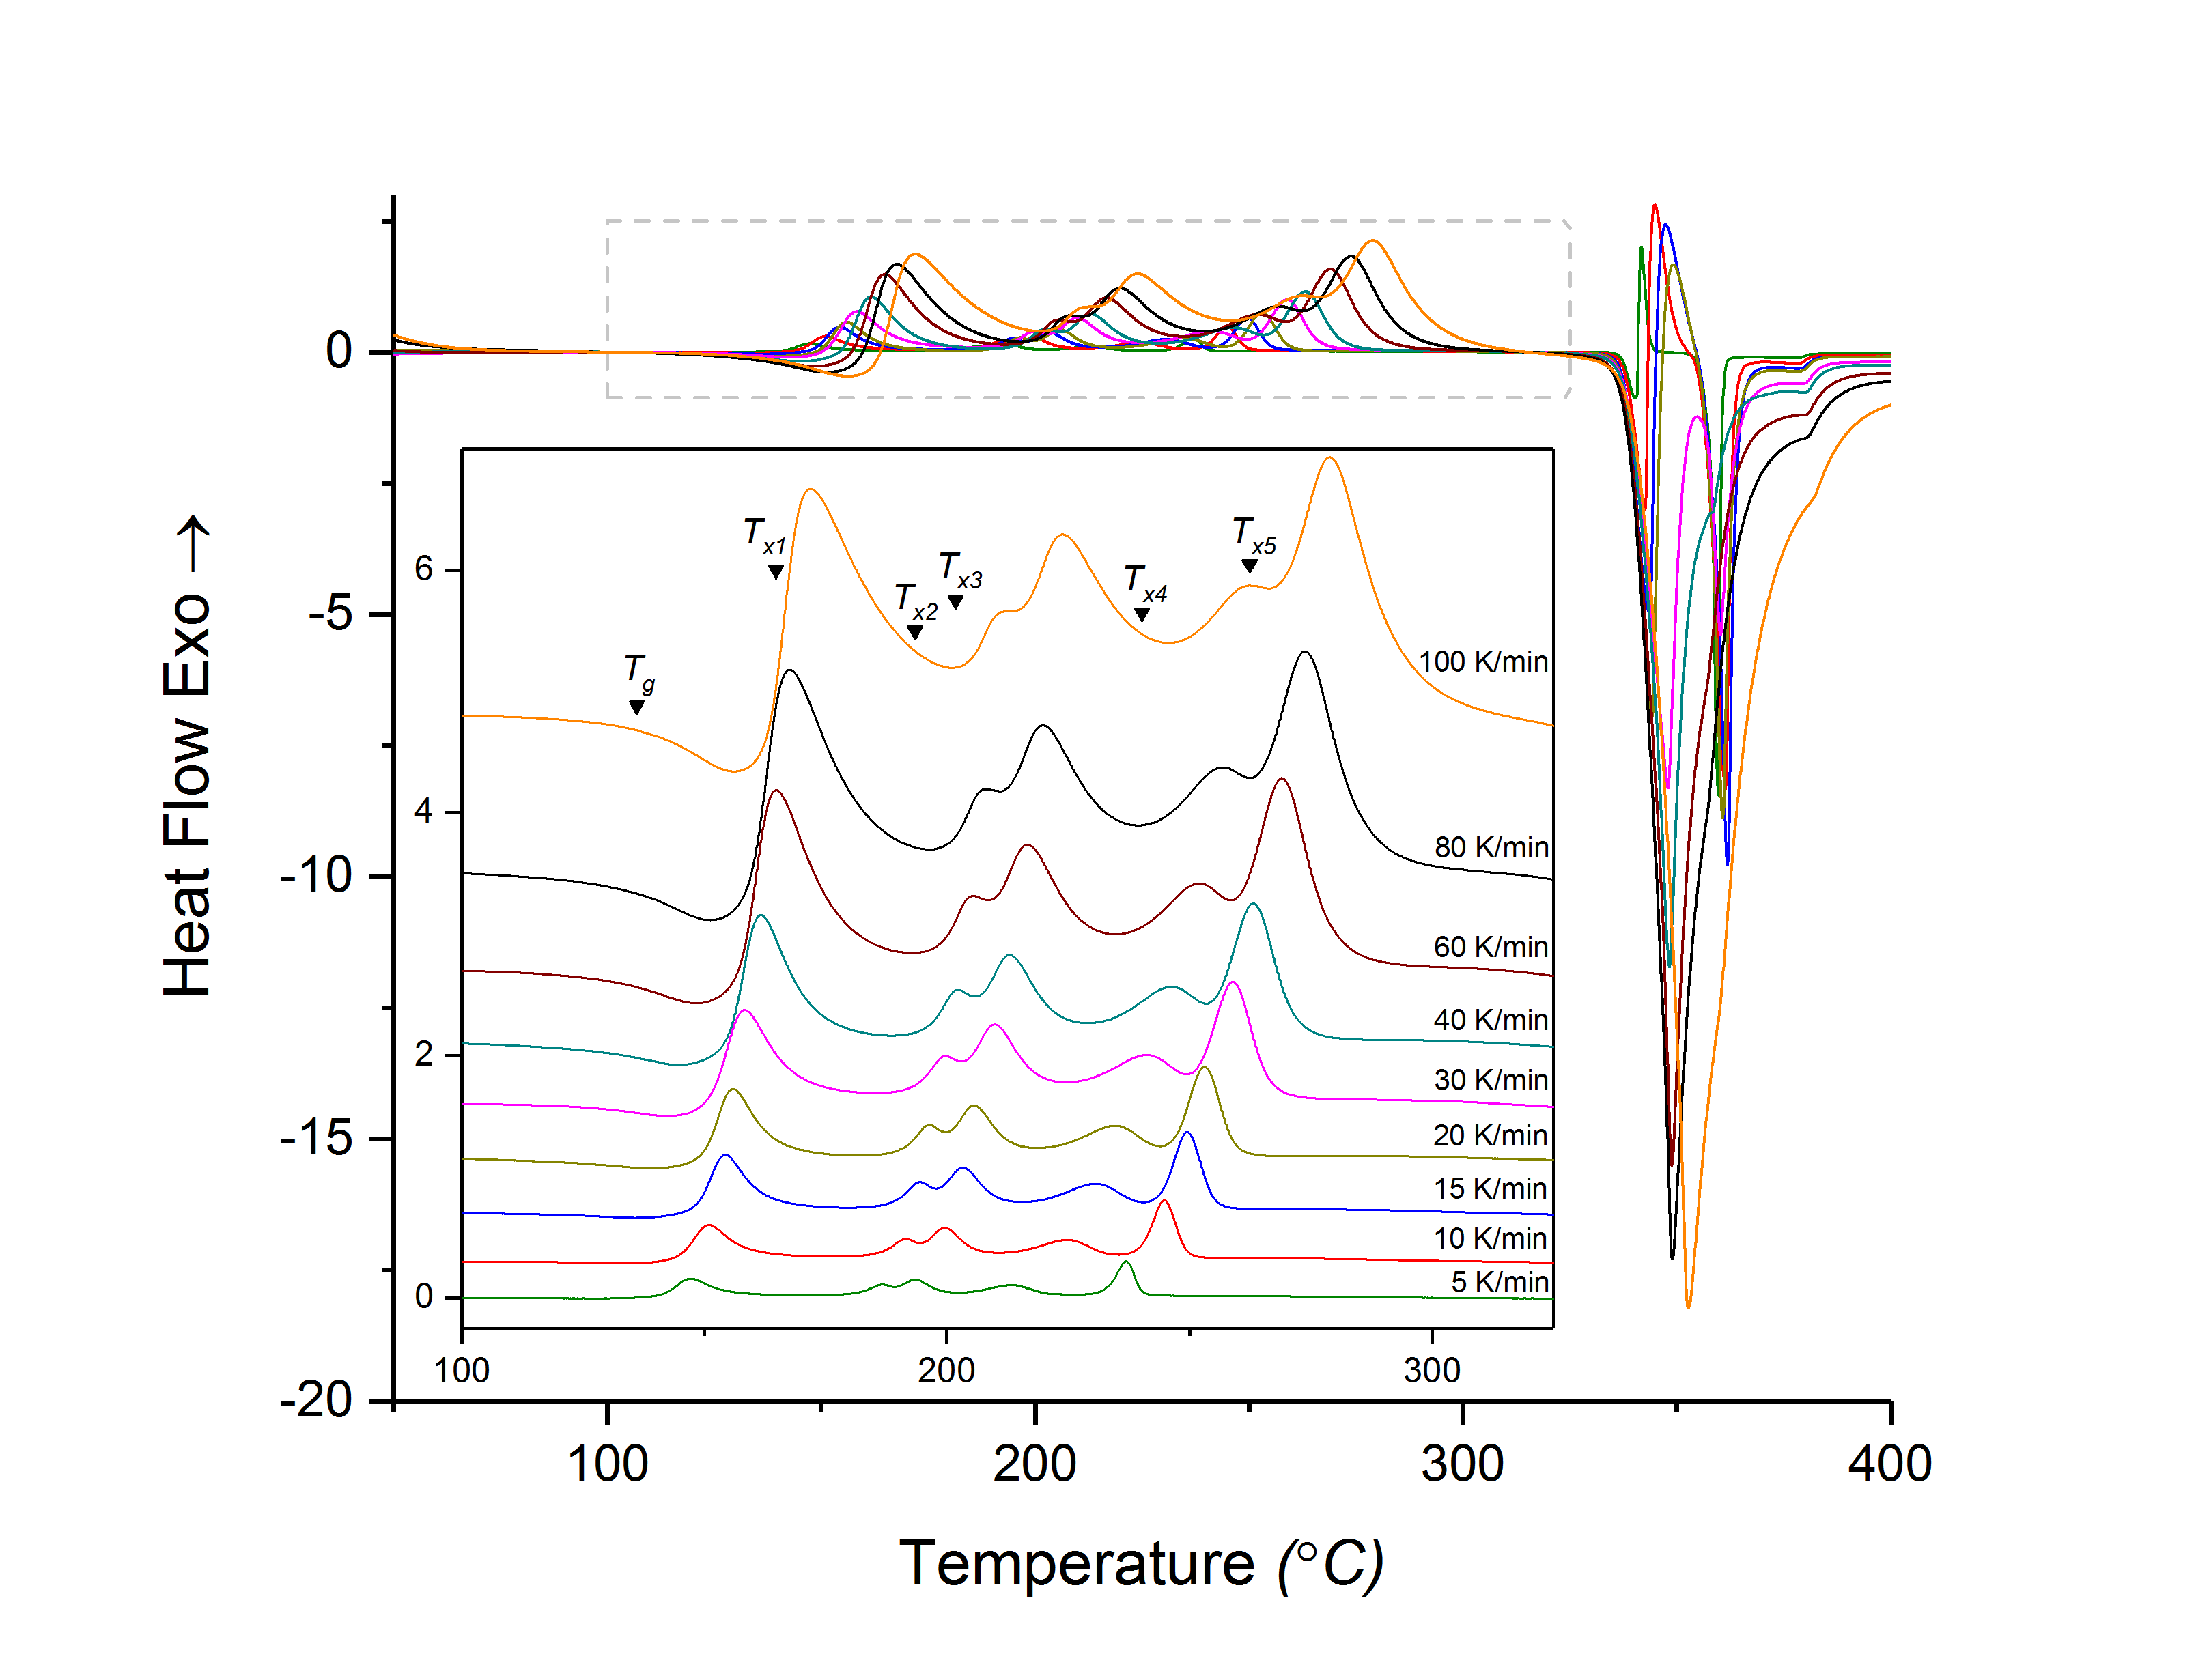
\includegraphics[width=0.65\textwidth]{DSC_Fragility_Bulk.png}
	\caption[Table of contents Capition]{Bulk \MgZnCa~ relaxed at 120 \degree C for 10 minutes and heated at various heating rates. The insert stacks the \gls{dsc} curves and labels the \Tg~ and \Tx es of the $100 K/min$ sample.}%global caption
	\label{fig:DSC_vHeatingRate_Bulk}
\end{figure}

%single image
\begin{figure}[b]
	\centering
	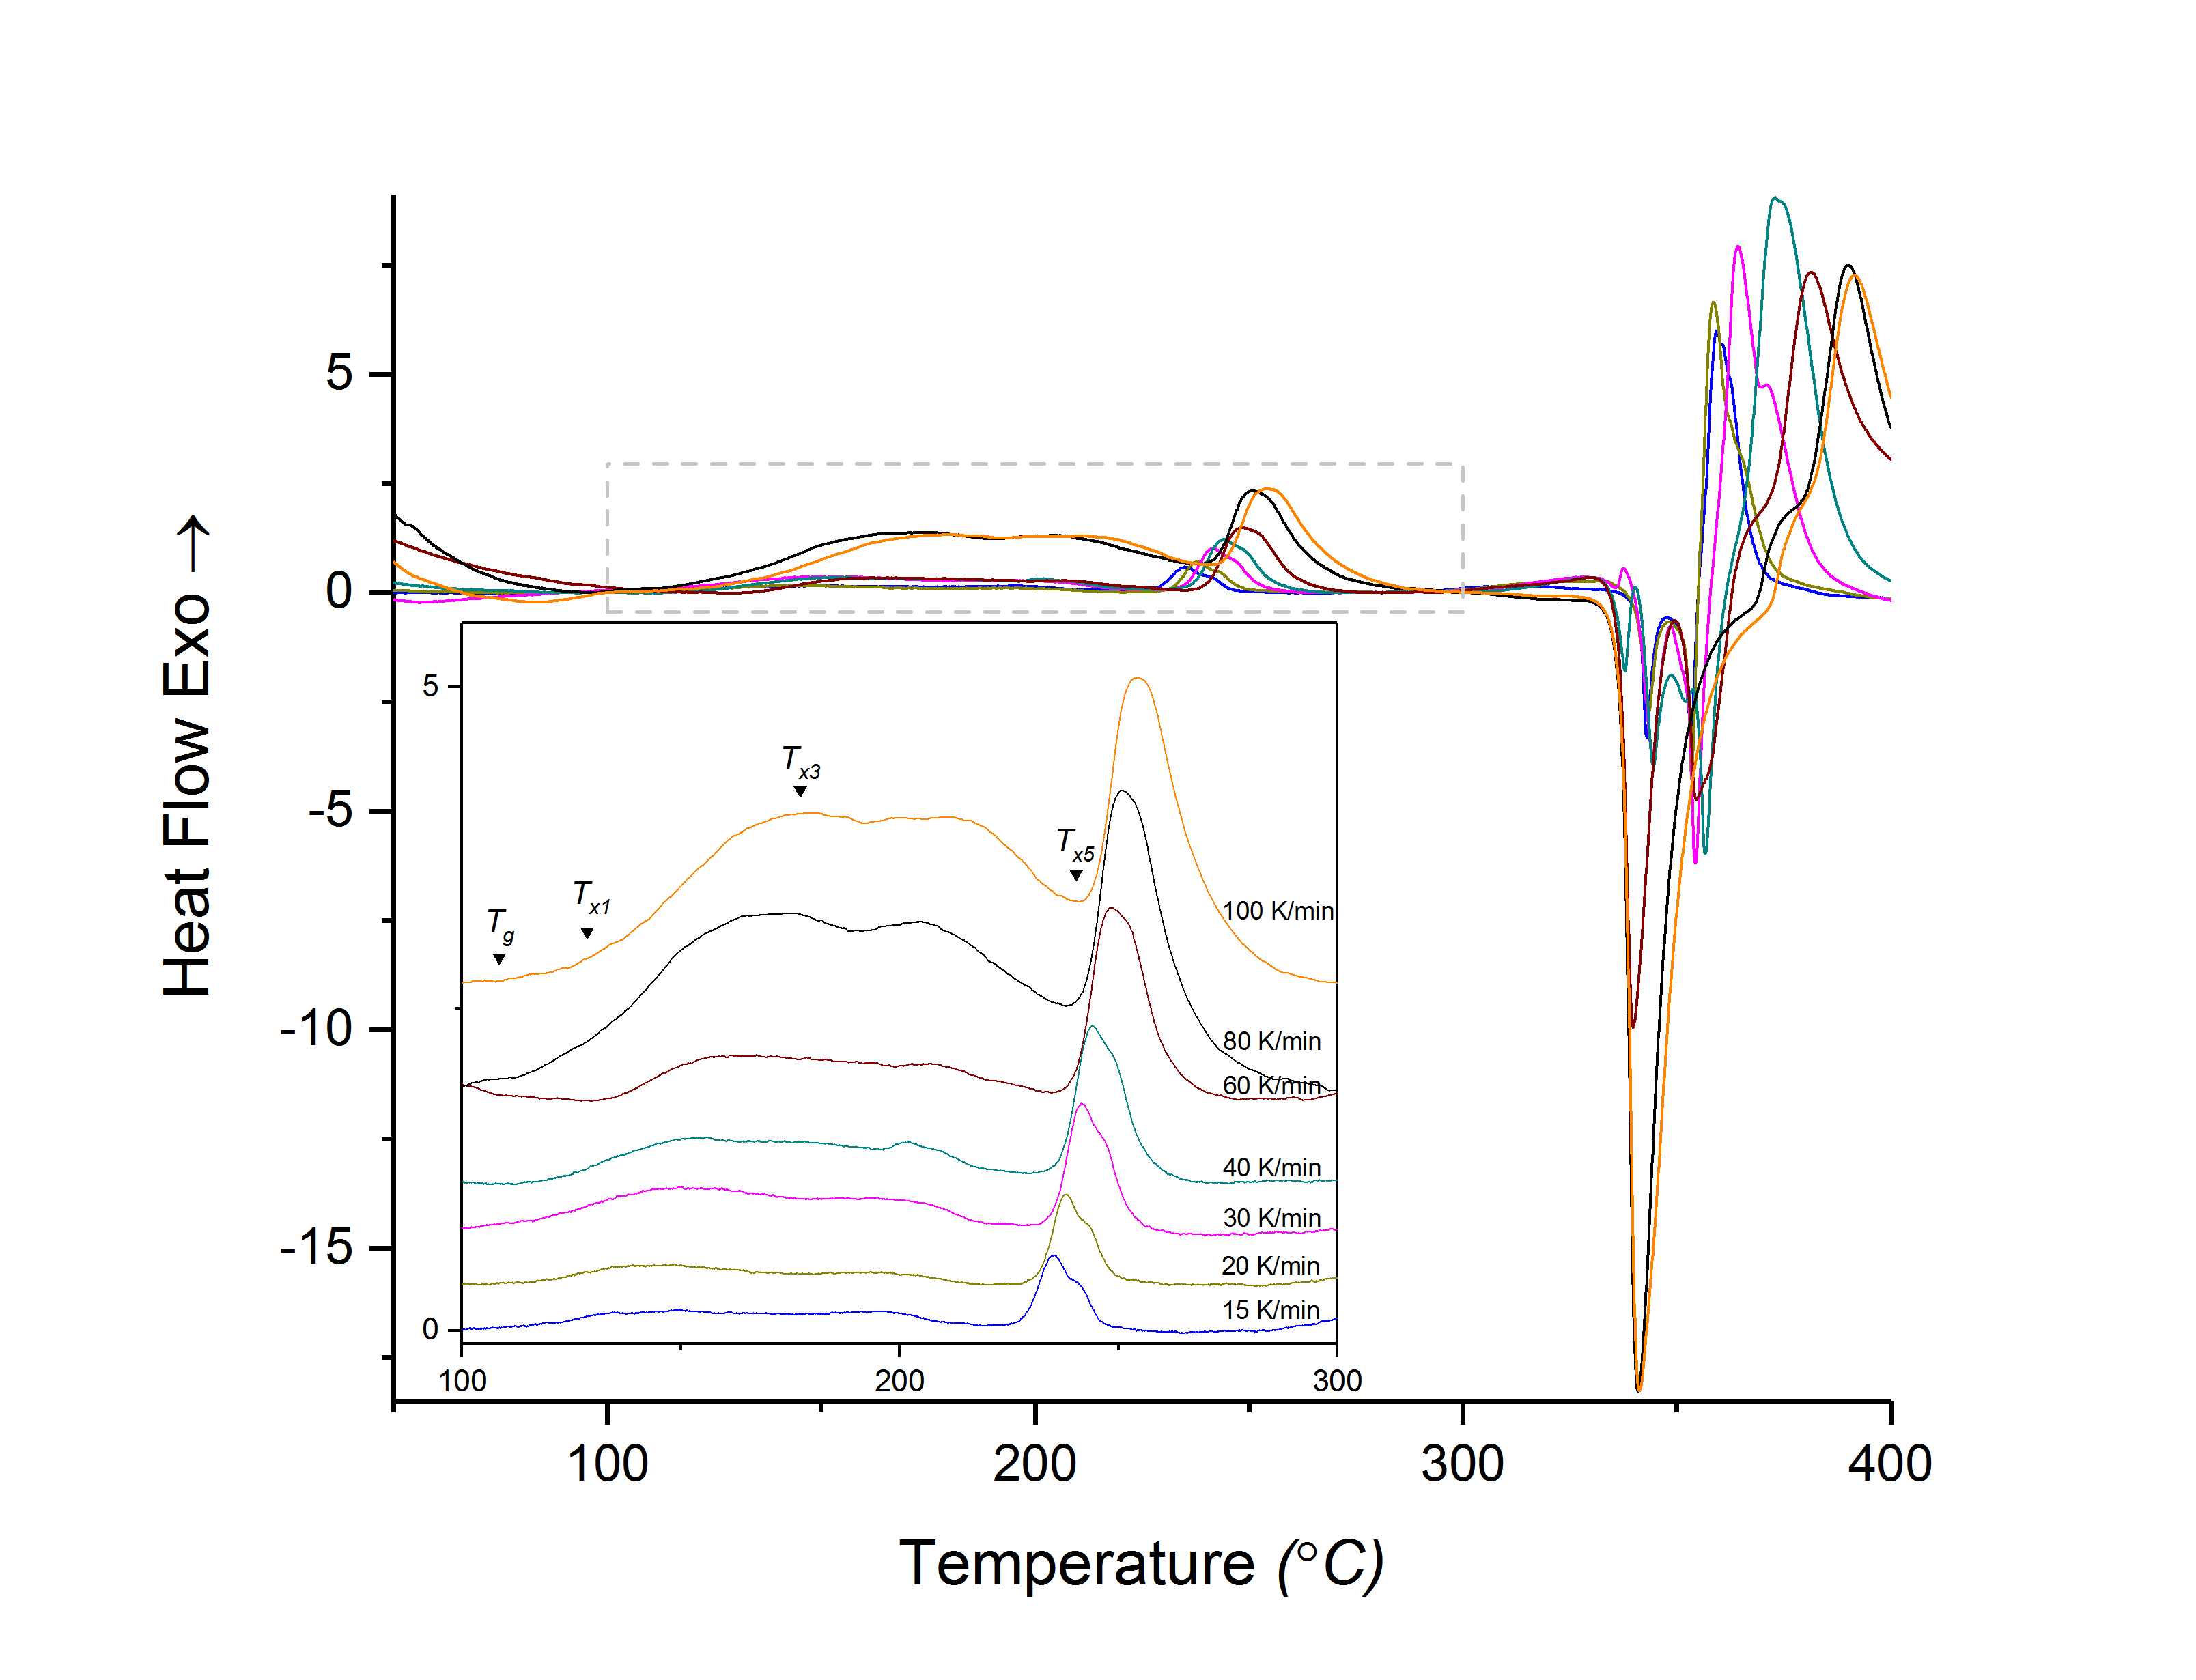
\includegraphics[width=0.65\textwidth]{DSC_Fragility_Film.png}
	\caption[Table of contents Capition]{Unrelaxed film \MgZnCa~ heated at various heating rates. The insert stacks the \gls{dsc} curves and labels the \Tg~ and \Tx es of the $100 K/min$ sample.}%global caption
	\label{fig:DSC_vHeatingRate_Film}
\end{figure}

\subsubsection{Fragility}

Using the isochronic \acrshort{dsc} data the \gls{m} of the \MgZnCa~ system could be established for both the bulk and film. Numerical solutions where used to fit the \acrshort{dsc} variant of the \gls{vft} relationship for \gls{ht} \cite{Busch1998}.

\begin{equation}
	\beta^{-1} = \tau_{0}~ e^{(\frac{D^{*}T_{0}}{T_{g}-T_{0}})}
	\label{equ:VFT}
\end{equation}

Where $\tau_{0}$ is a pre-exponential factor, $D^{*}$ is the liquid \acrlong{m} parameter, and $T_{0}$ is the \gls{vft} temperature where the barrier to flow becomes infinite.

The \gls{m} could then be calculated from Equation \ref{equ:dStar} \cite{Angell2002, Wei2014}.

\begin{equation}
	D^{*}=590/(m-16)
	\label{equ:dStar}
\end{equation}

Using these two equations for the bulk it was found $\beta^{-1} = 1.338E - 16e^{5274 (\frac{1}{T-T_{0}})}$ with an Adj. $R^{2}=0.972$. This gave a $D^{*}=20.4$, and a \gls{m}$=44.9$. The film was fitted to $\beta^{-1} = 5.921E - 11e^{2766 (\frac{1}{T-T_{0}})}$ with a lower confidence of Adj. $R^{2}=0.861$, likely owing to the reduced number of data points. This gave a $D^{*}=10.0$, and \gls{m}$=75.0$, see Figure \ref{fig:Fragility_BulkFilm_mValue}.

%single image
\begin{figure}[b]
	\centering
	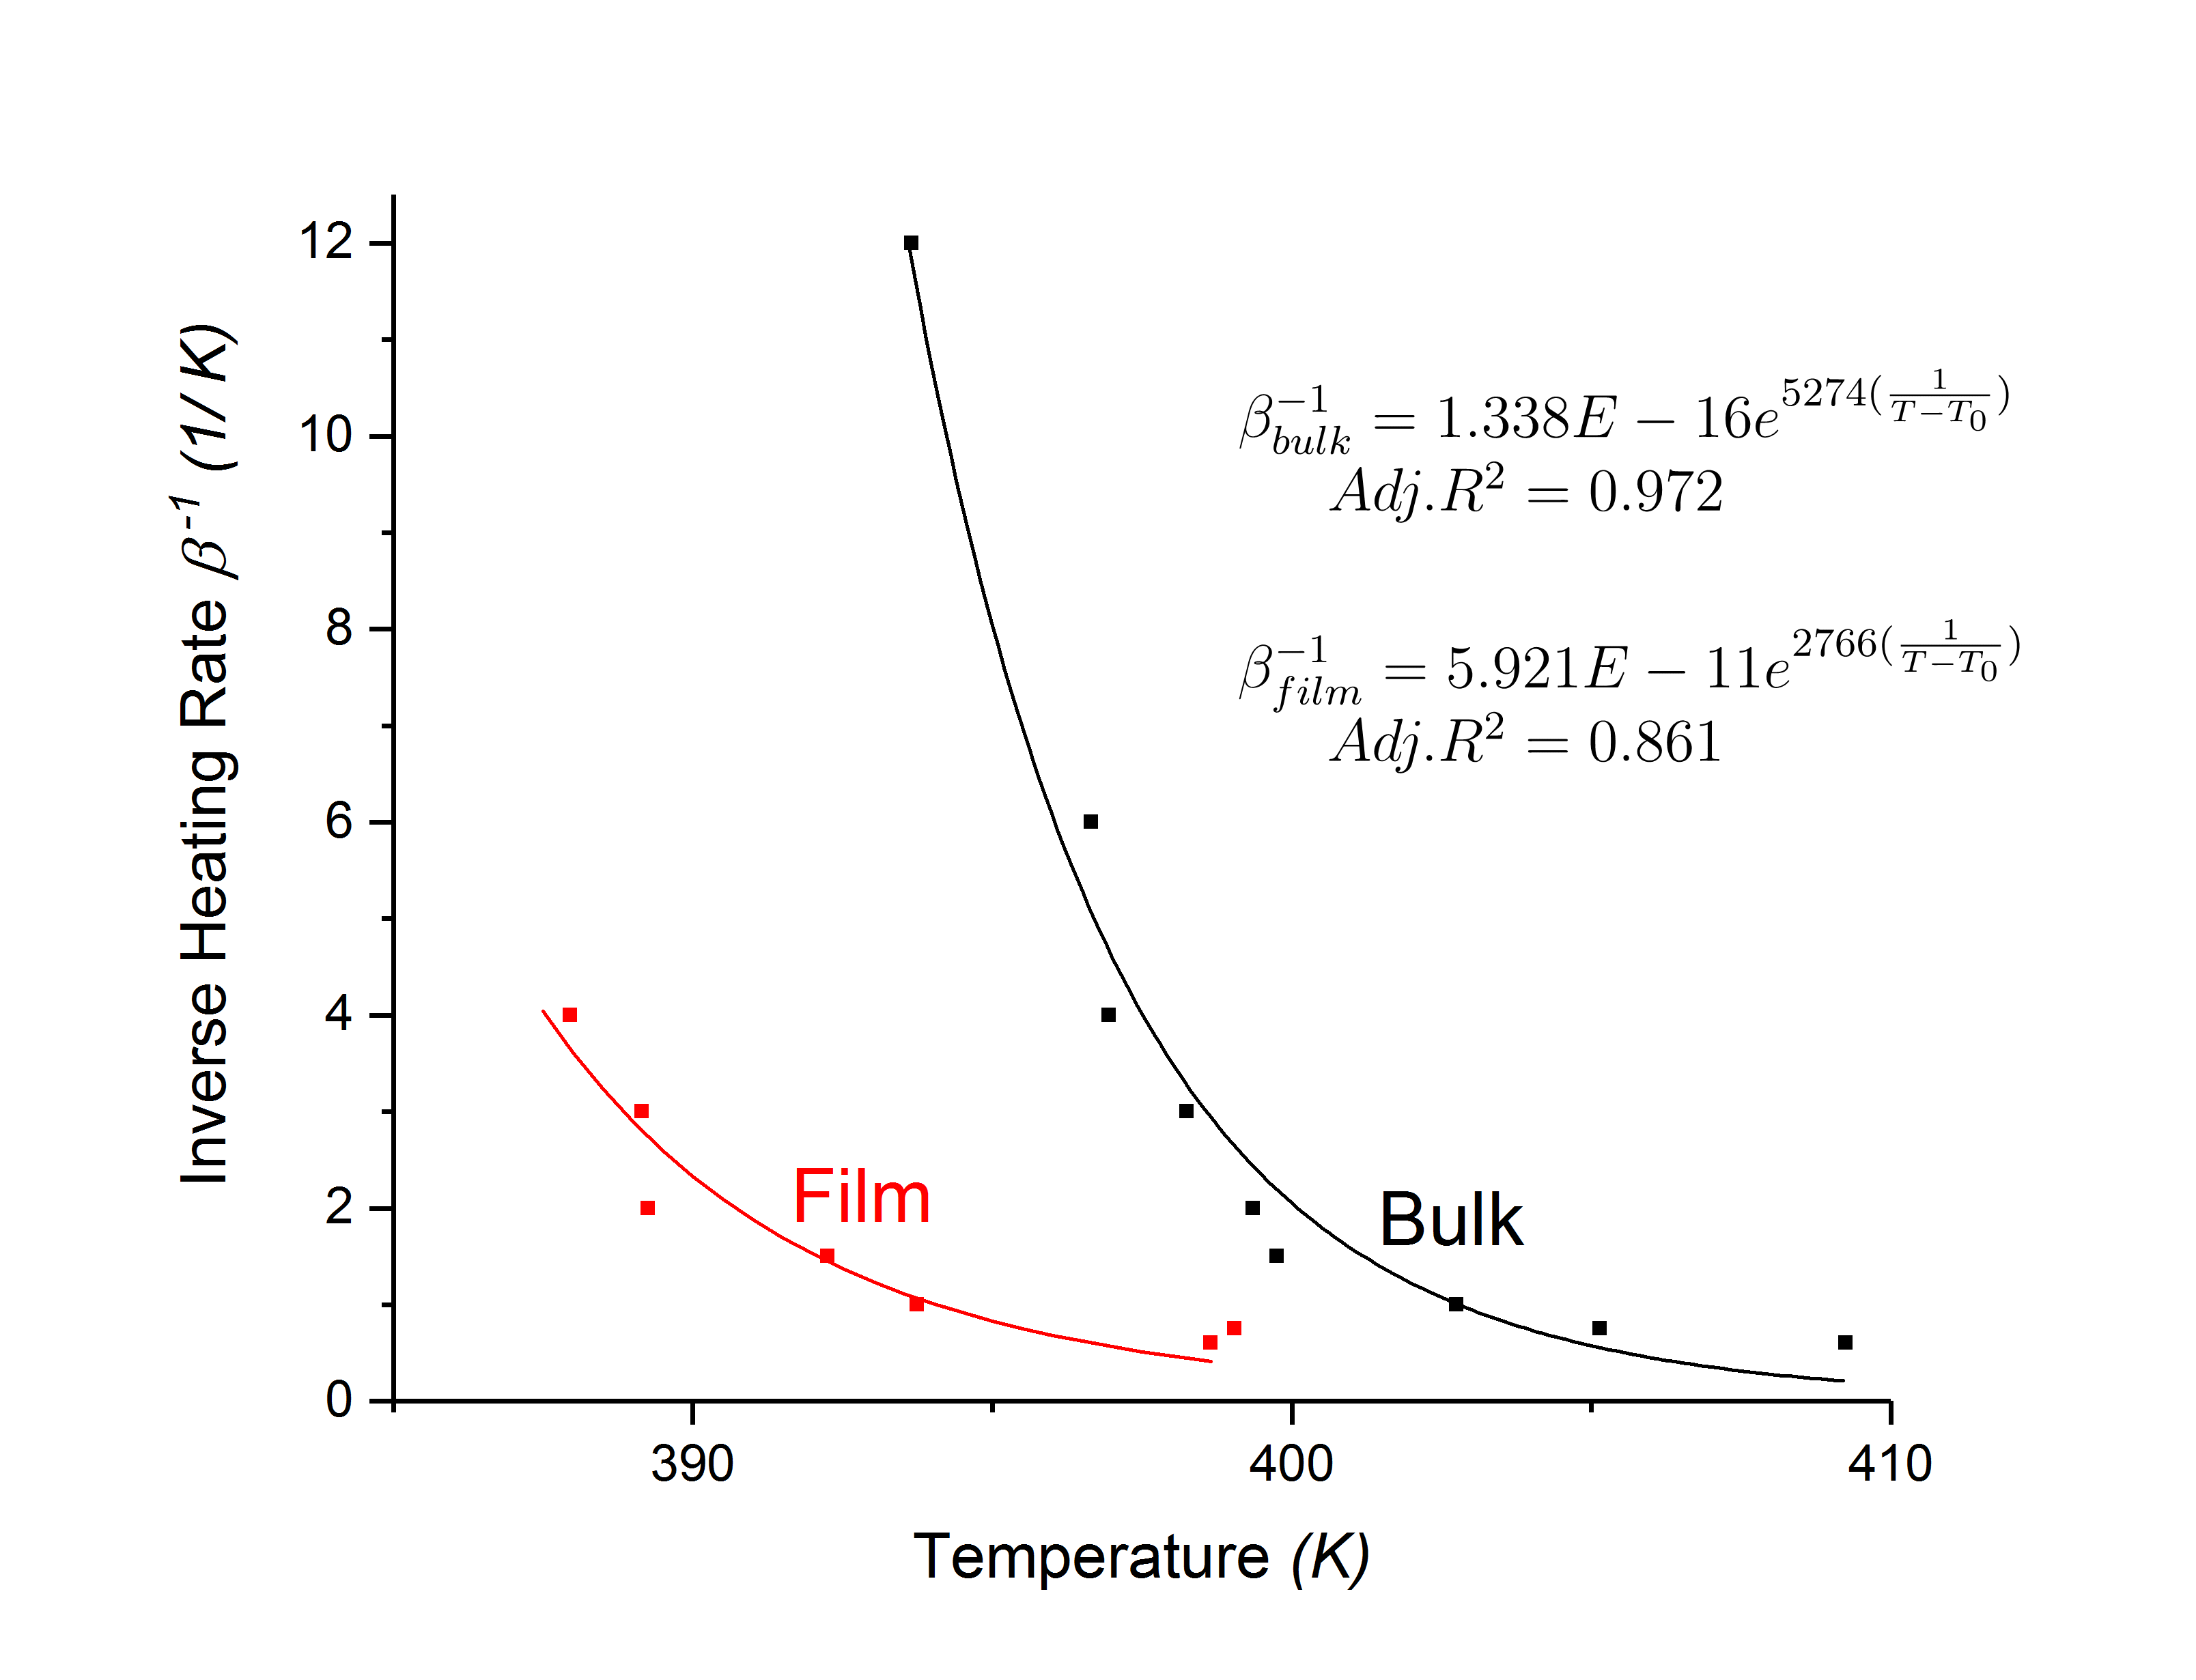
\includegraphics[width=0.95\textwidth]{Bulk_Film_Fragility.png}
	\caption[Table of contents Capition]{Fitted \acrfull{m} for the \MgZnCa system obtained by \acrshort{dsc} at various heating rates}
	\label{fig:Fragility_BulkFilm_mValue}
\end{figure}

\subsection{\acrshort{dsc} deconvolution}

%MultiFigure
\begin{figure}[b]
	\centering
	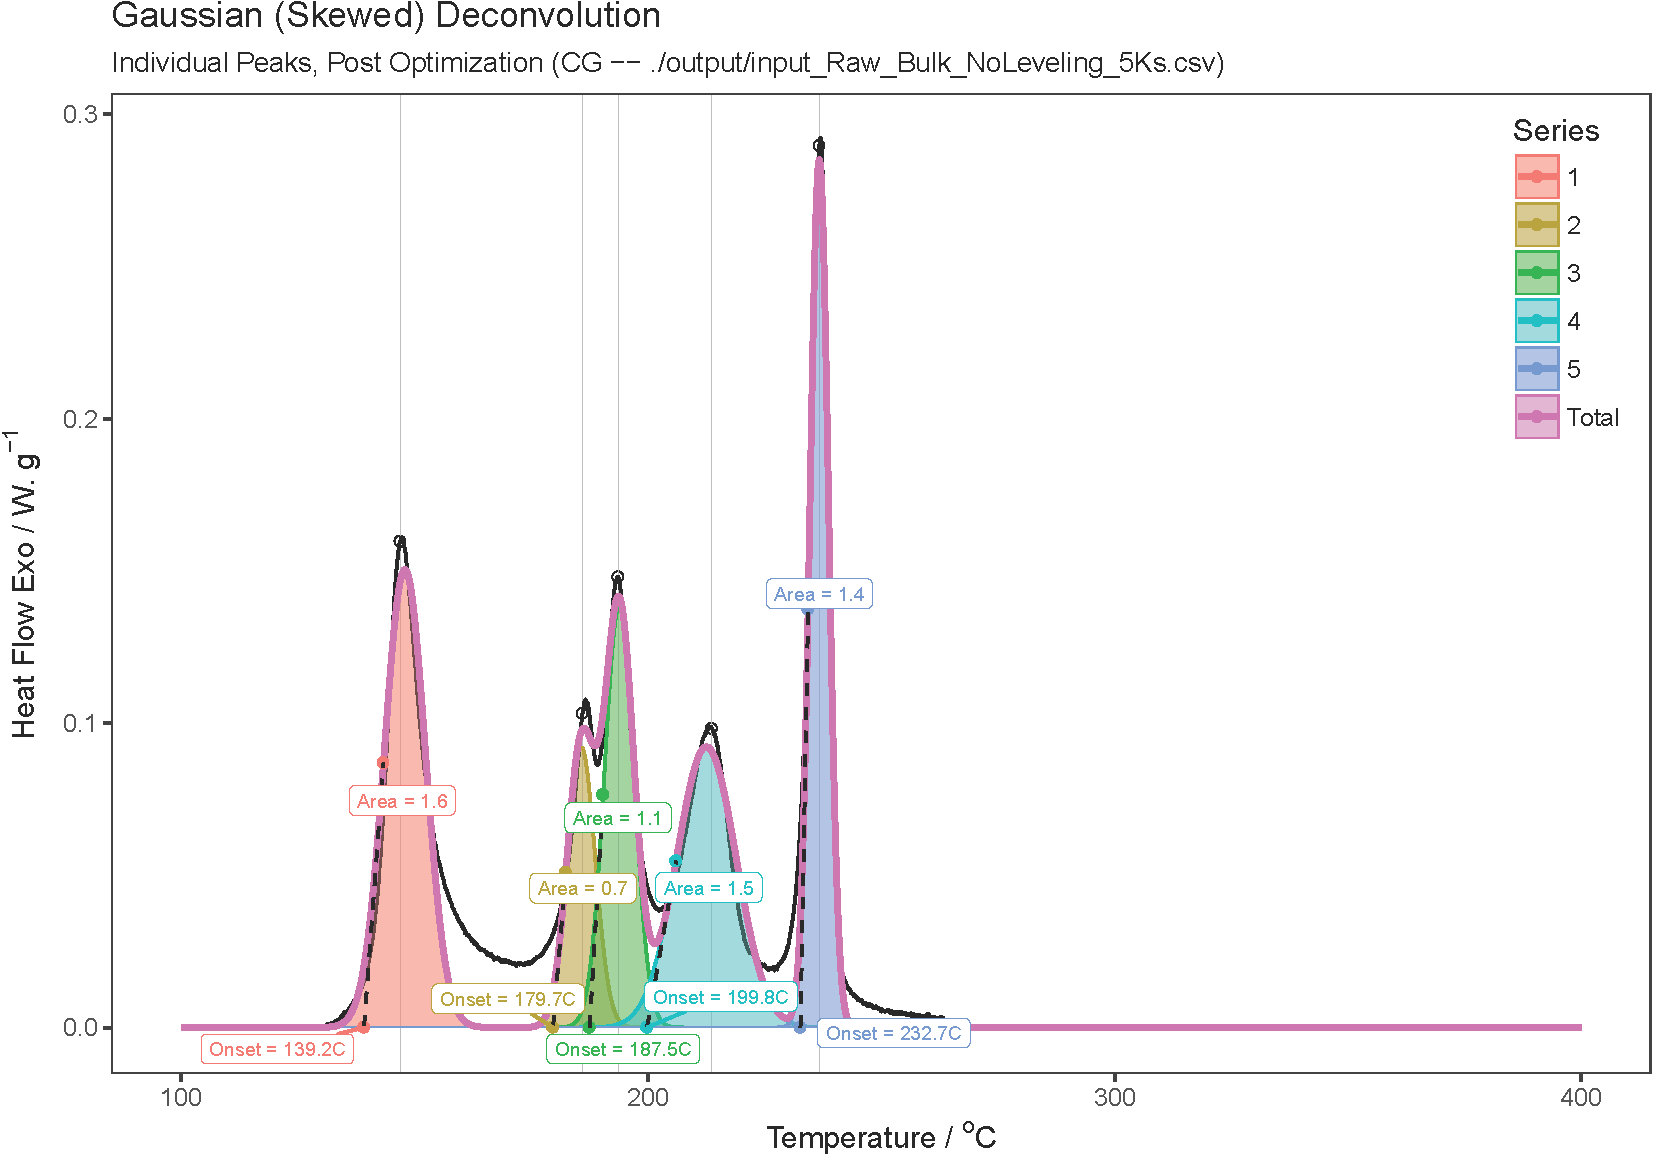
\includegraphics[width=.3\textwidth]{input_Raw_Bulk_NoLeveling_5Ks_result_A5lsc.png}\quad
	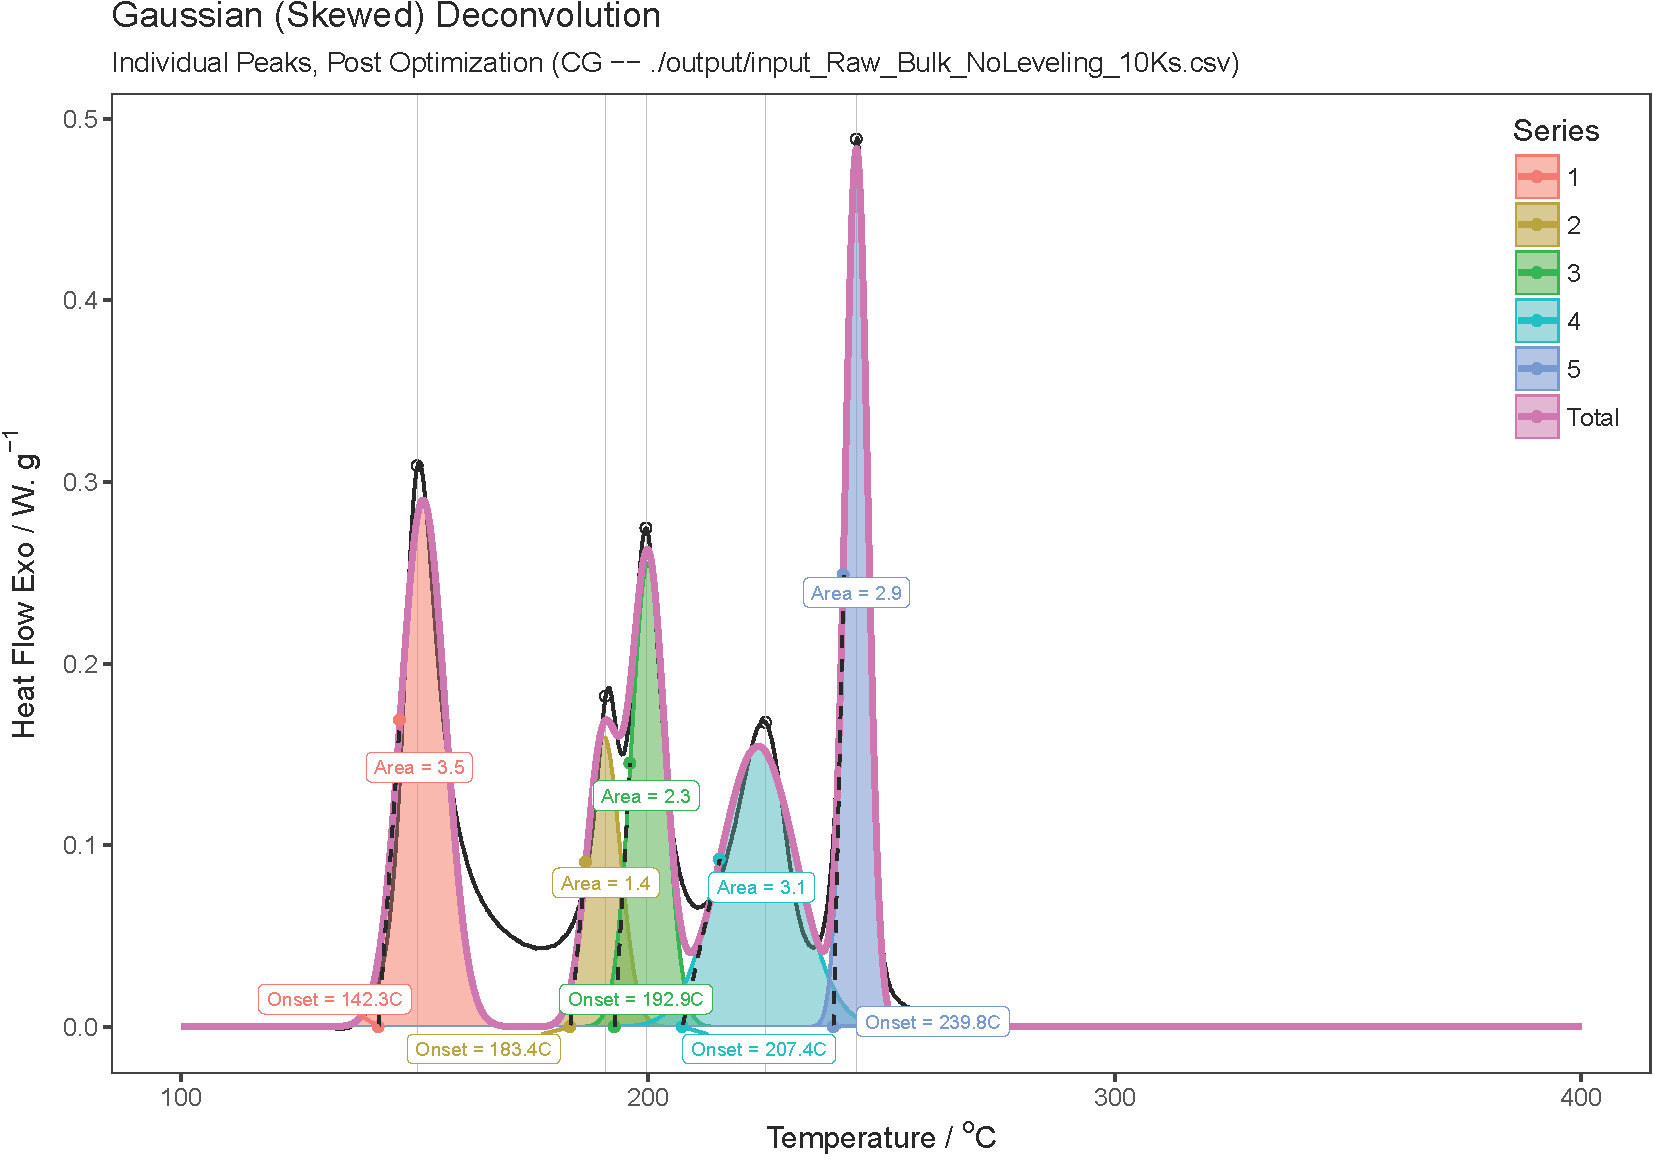
\includegraphics[width=.3\textwidth]{input_Raw_Bulk_NoLeveling_10Ks_result_A5lsc.png}\quad
	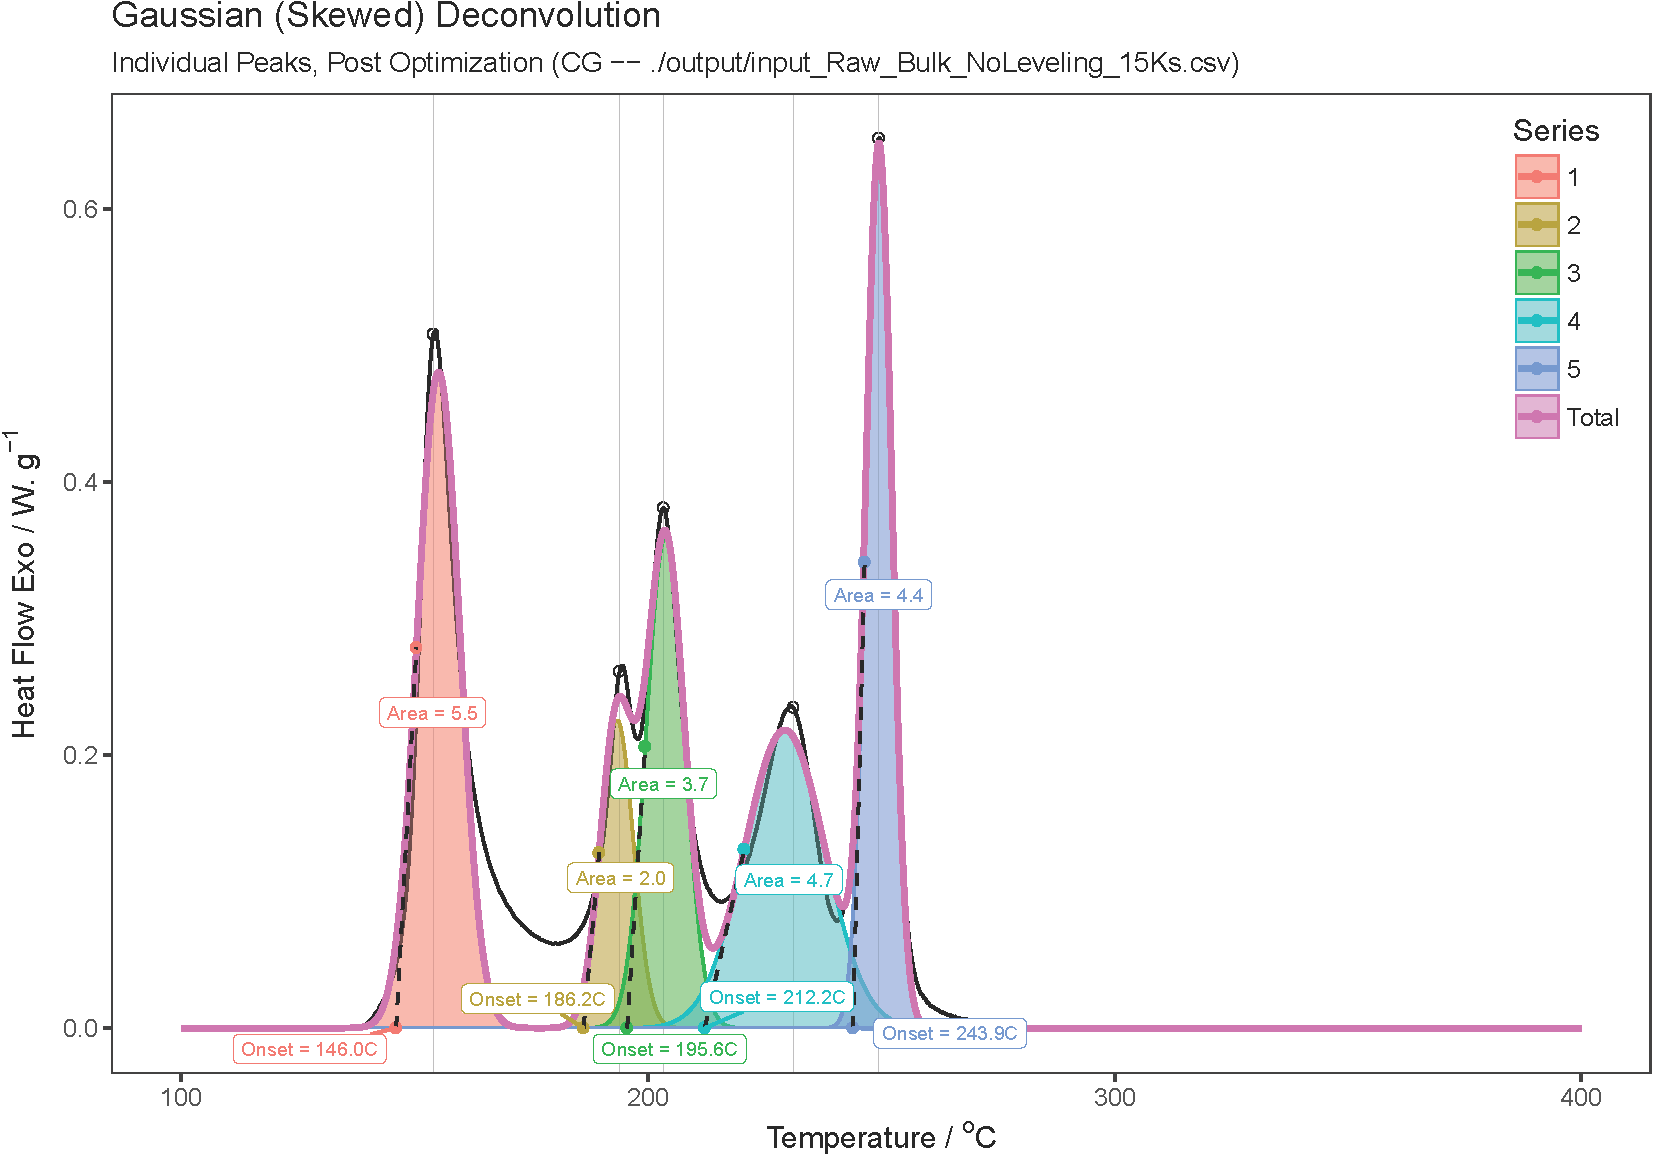
\includegraphics[width=.3\textwidth]{input_Raw_Bulk_NoLeveling_15Ks_result_A5lsc.png}
	\medskip
	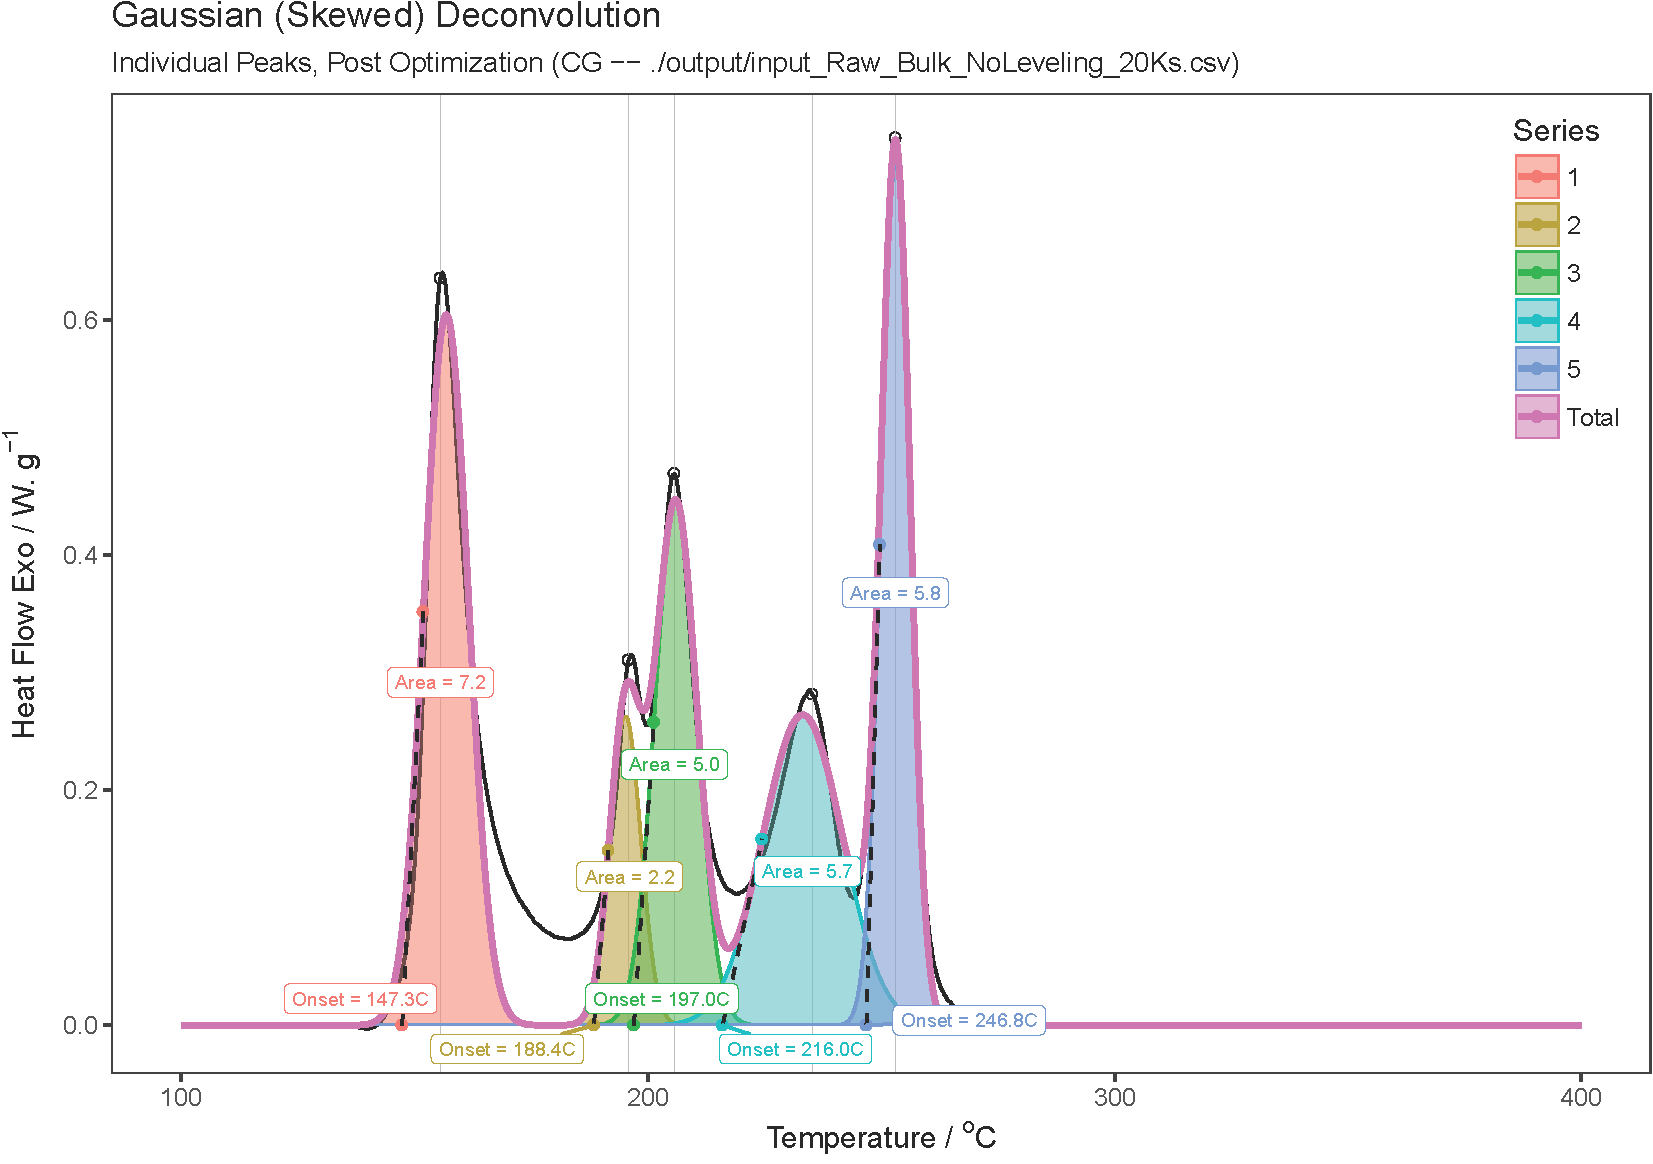
\includegraphics[width=.3\textwidth]{input_Raw_Bulk_NoLeveling_20Ks_result_A5lsc.png}\quad
	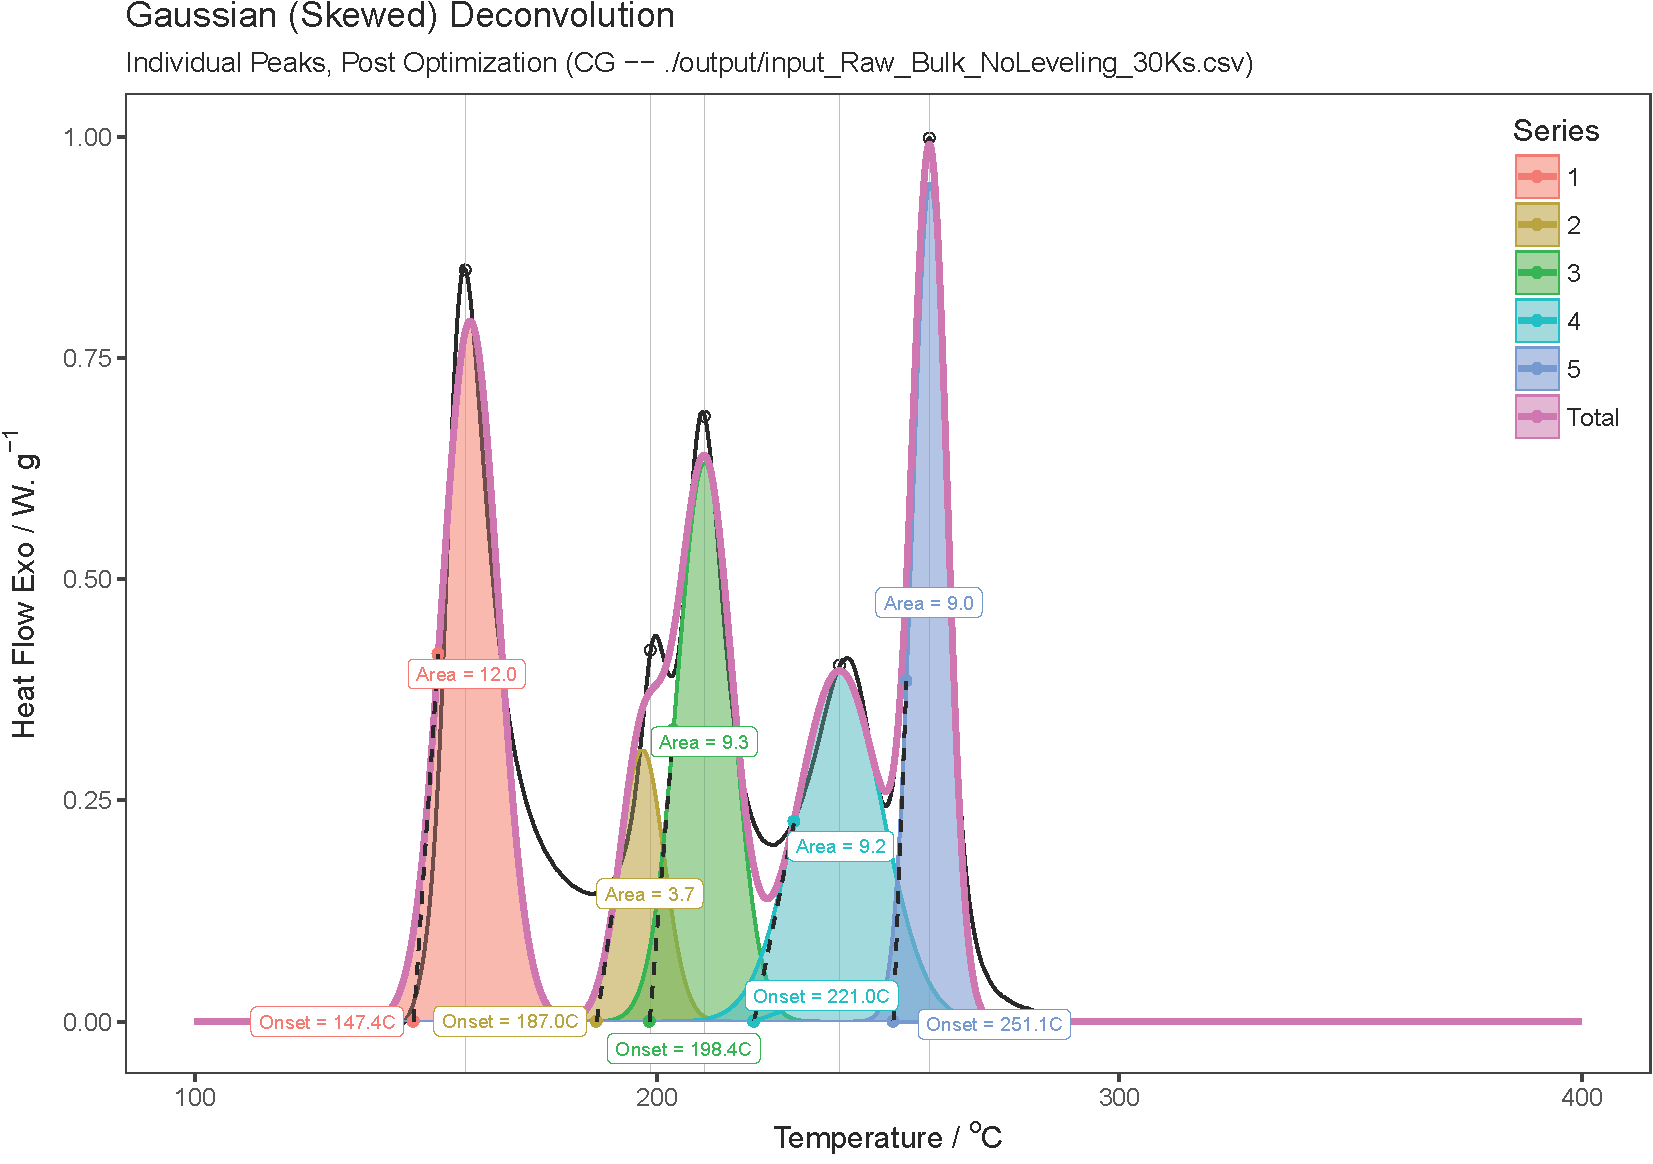
\includegraphics[width=.3\textwidth]{input_Raw_Bulk_NoLeveling_30Ks_result_A5lsc.png}\quad
	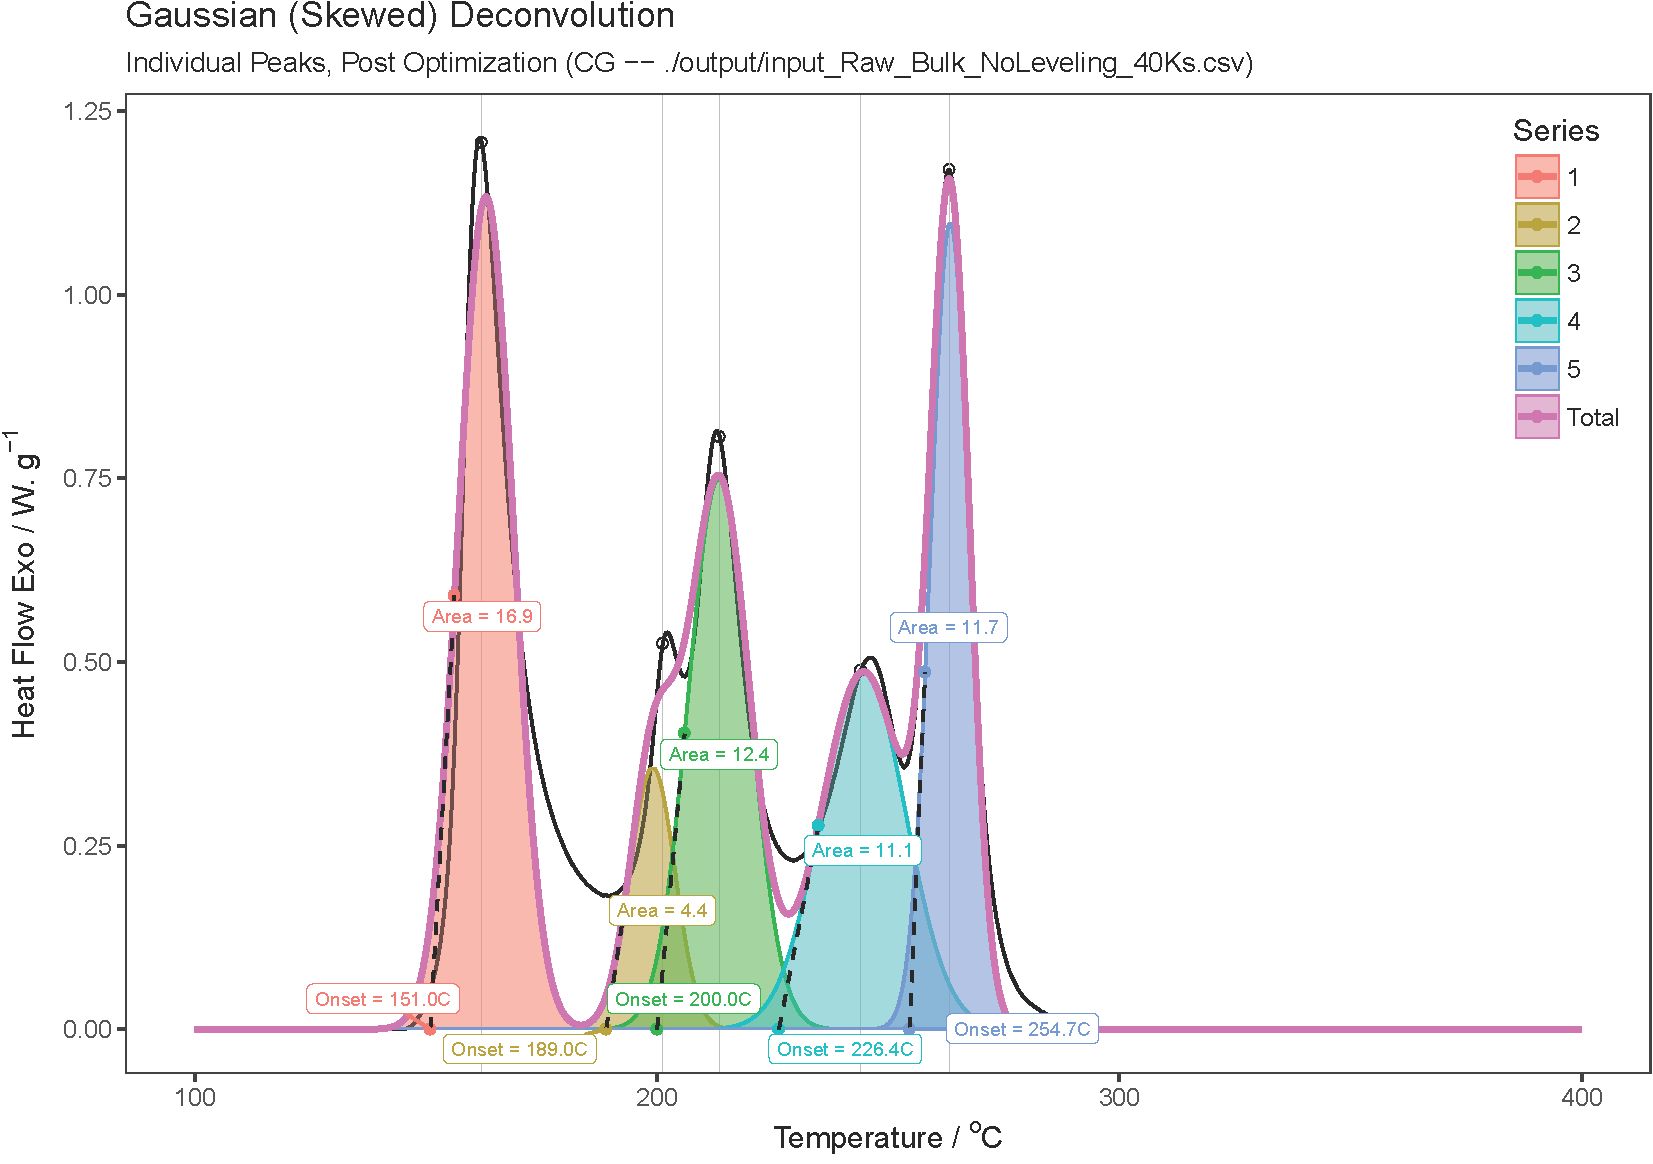
\includegraphics[width=.3\textwidth]{input_Raw_Bulk_NoLeveling_40Ks_result_A5lsc.png}
	\medskip
	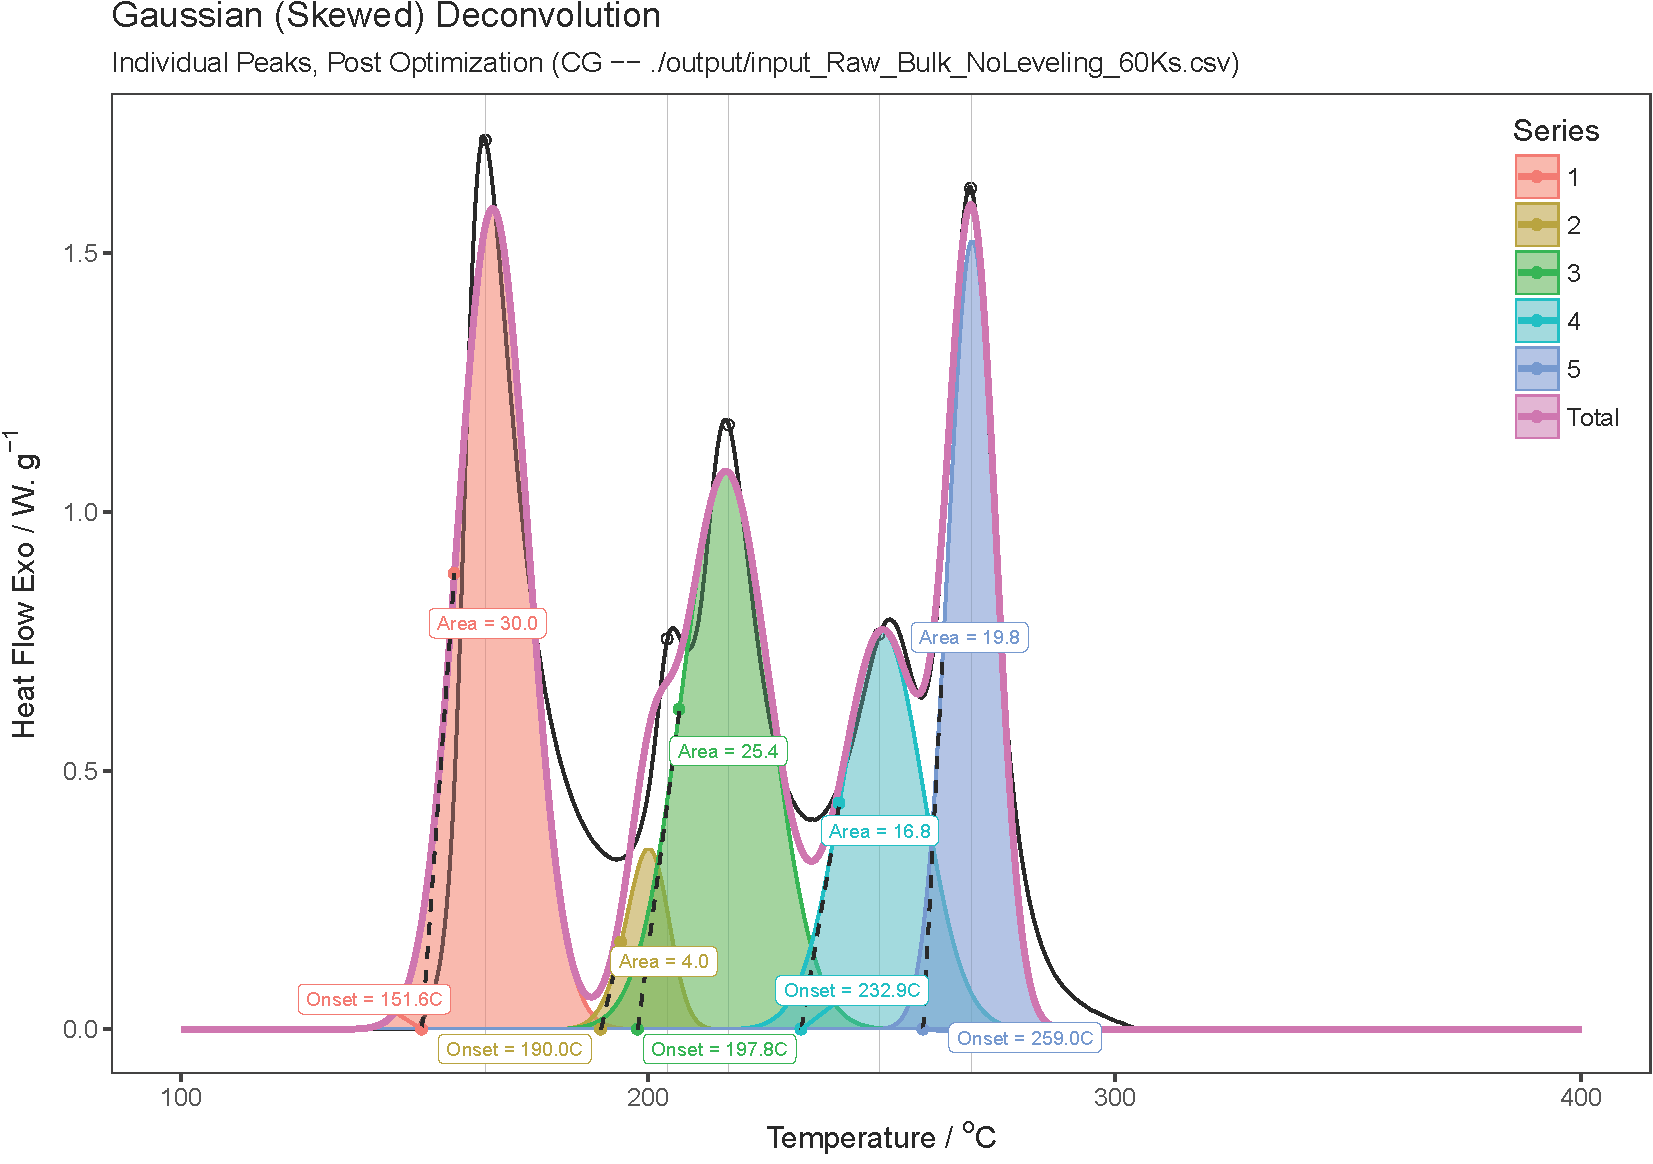
\includegraphics[width=.3\textwidth]{input_Raw_Bulk_NoLeveling_60Ks_result_A5lsc.png}\quad
	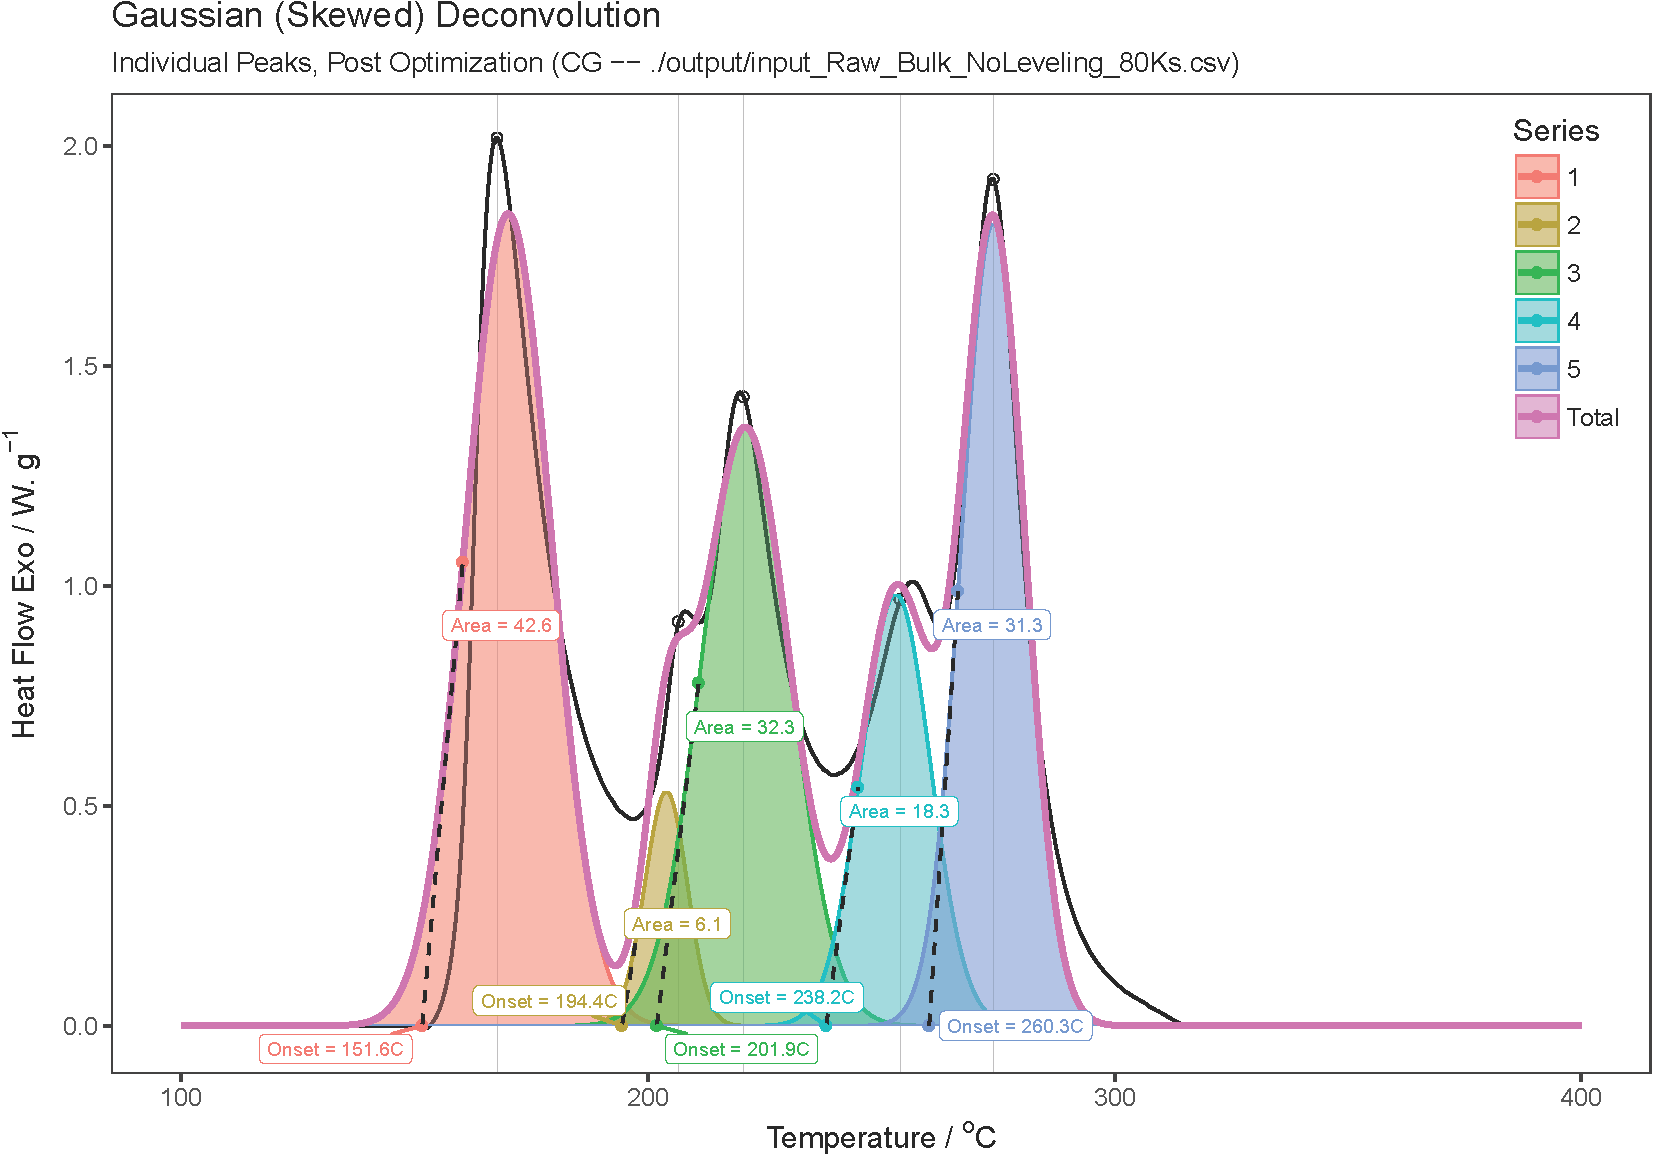
\includegraphics[width=.3\textwidth]{input_Raw_Bulk_NoLeveling_80Ks_result_A5lsc.png}\quad
	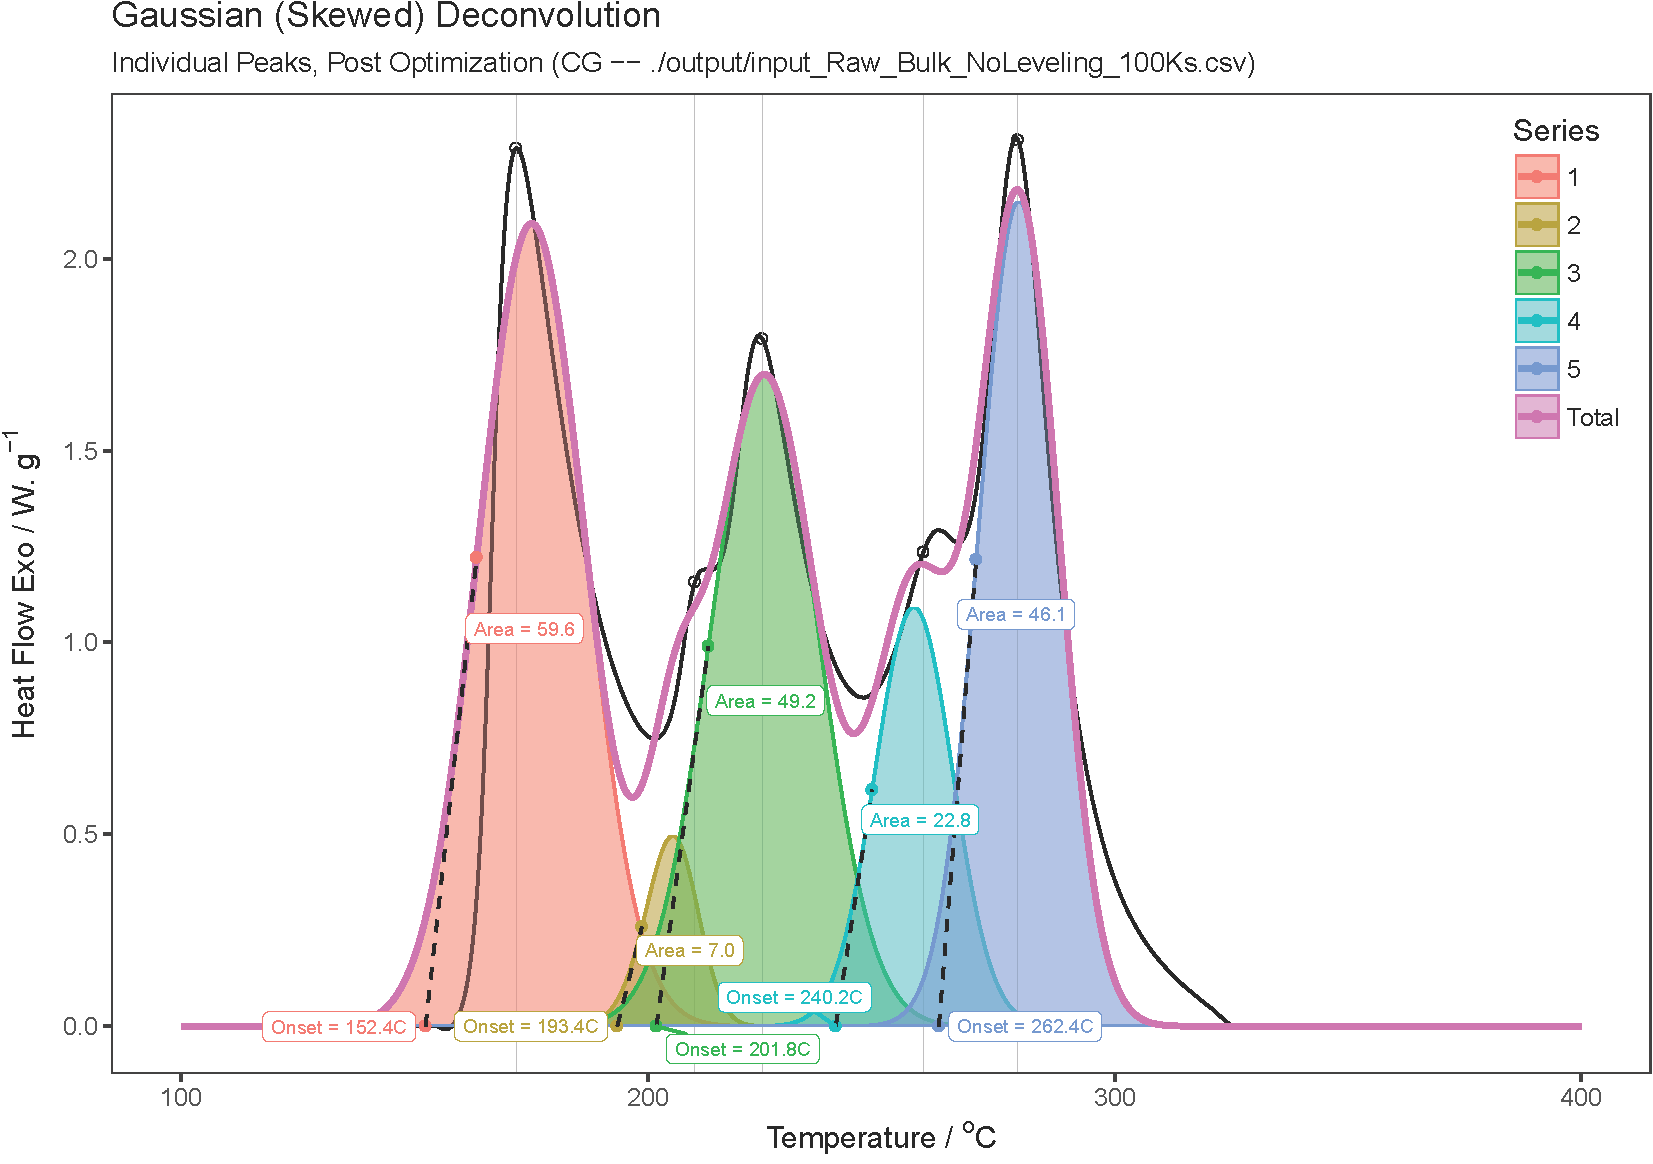
\includegraphics[width=.3\textwidth]{input_Raw_Bulk_NoLeveling_100Ks_result_A5lsc.png}
	\caption{\acrshort{dsc} deconvolution for the bulk. From left to right, top to bottom, 5, 10, 15, 20, 30, 40, 60, 80, 100 K/min.}
	\label{fig:DSC_Bulk_Decon}
\end{figure}

%MultiFigure
\begin{figure}[b]
	\centering
	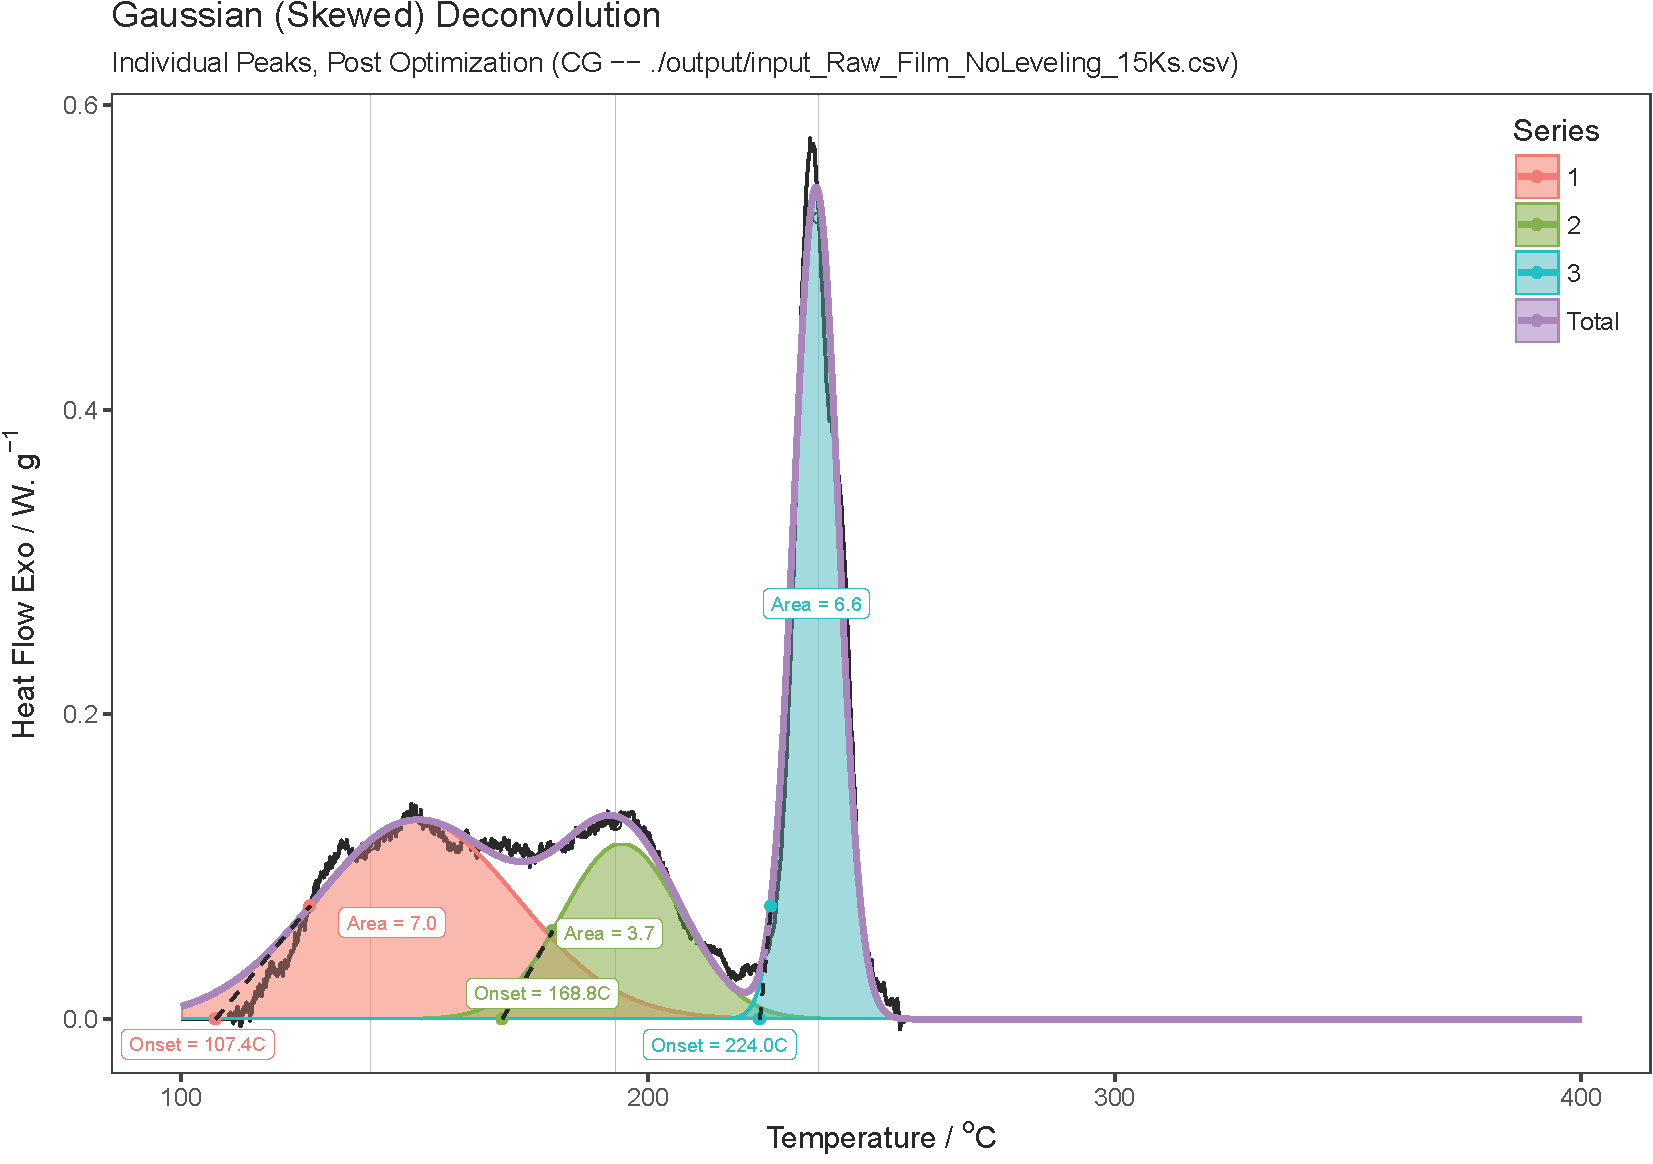
\includegraphics[width=.3\textwidth]{input_Raw_Film_NoLeveling_15Ks_result_A5lsc.png}\quad
	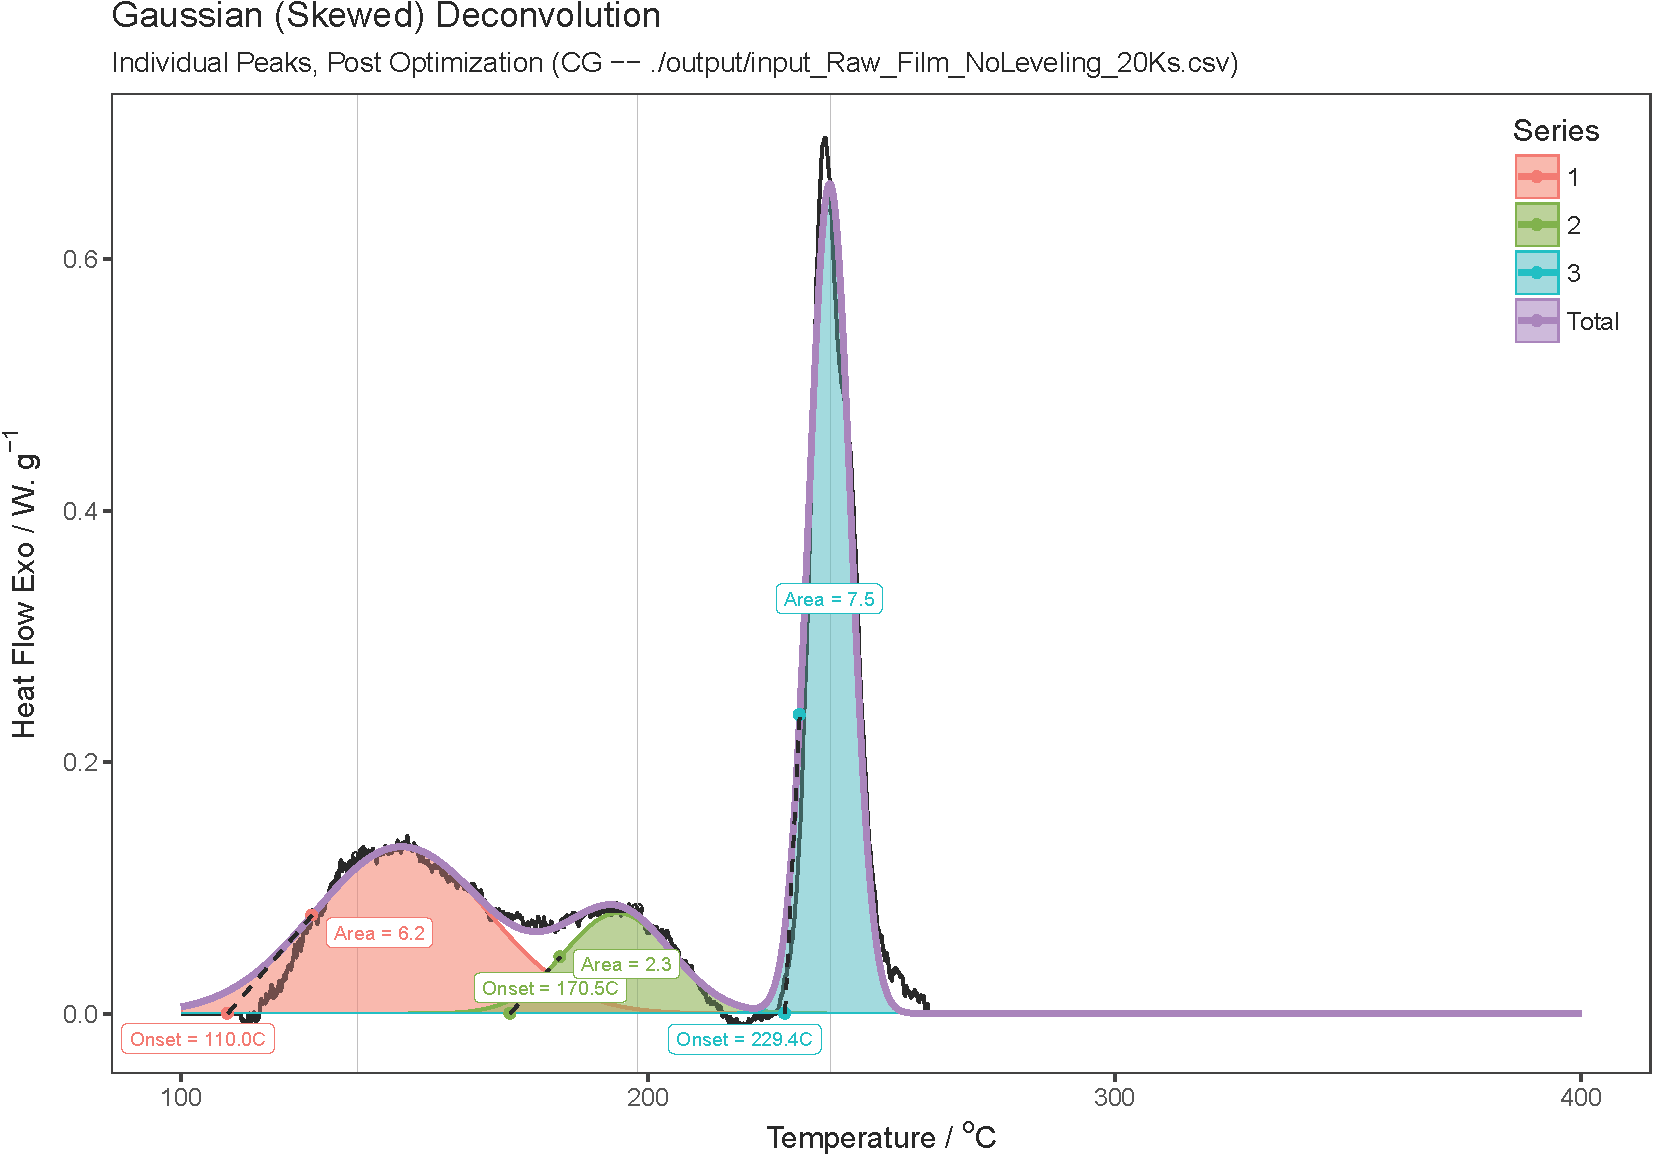
\includegraphics[width=.3\textwidth]{input_Raw_Film_NoLeveling_20Ks_result_A5lsc.png}\quad
	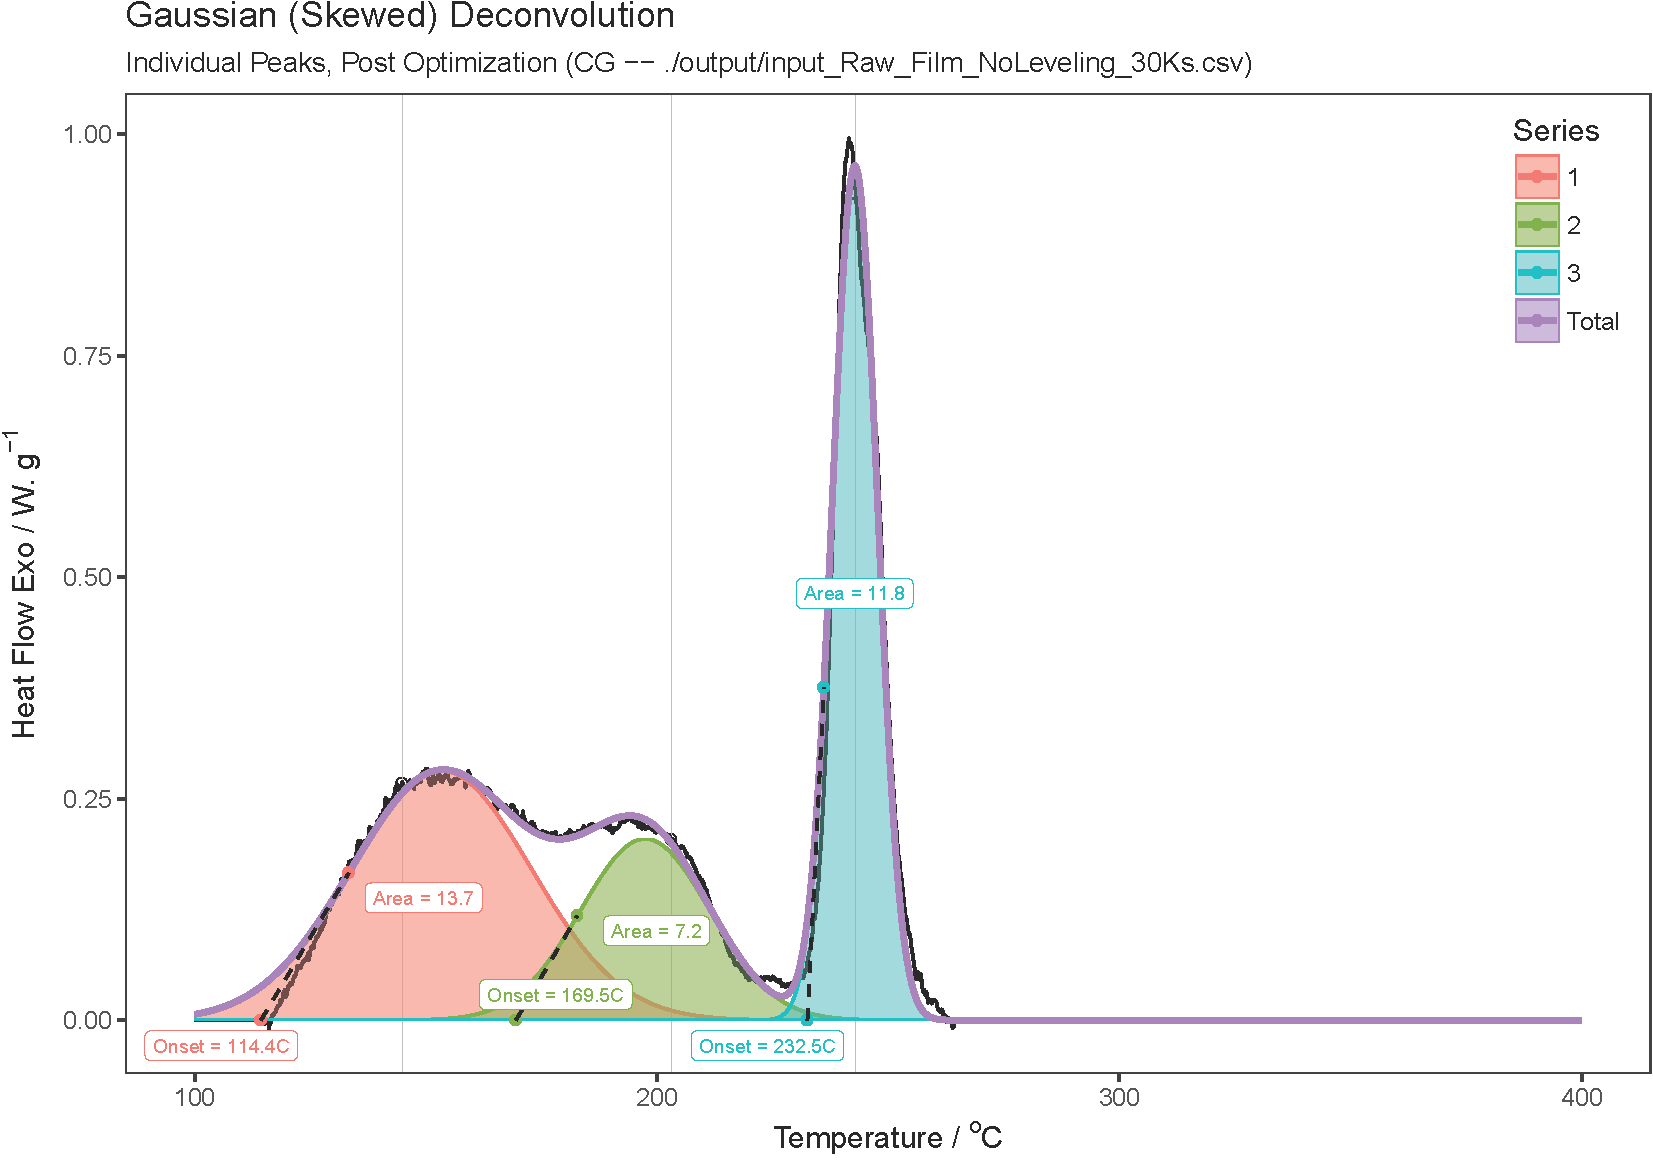
\includegraphics[width=.3\textwidth]{input_Raw_Film_NoLeveling_30Ks_result_A5lsc.png}
	\medskip
	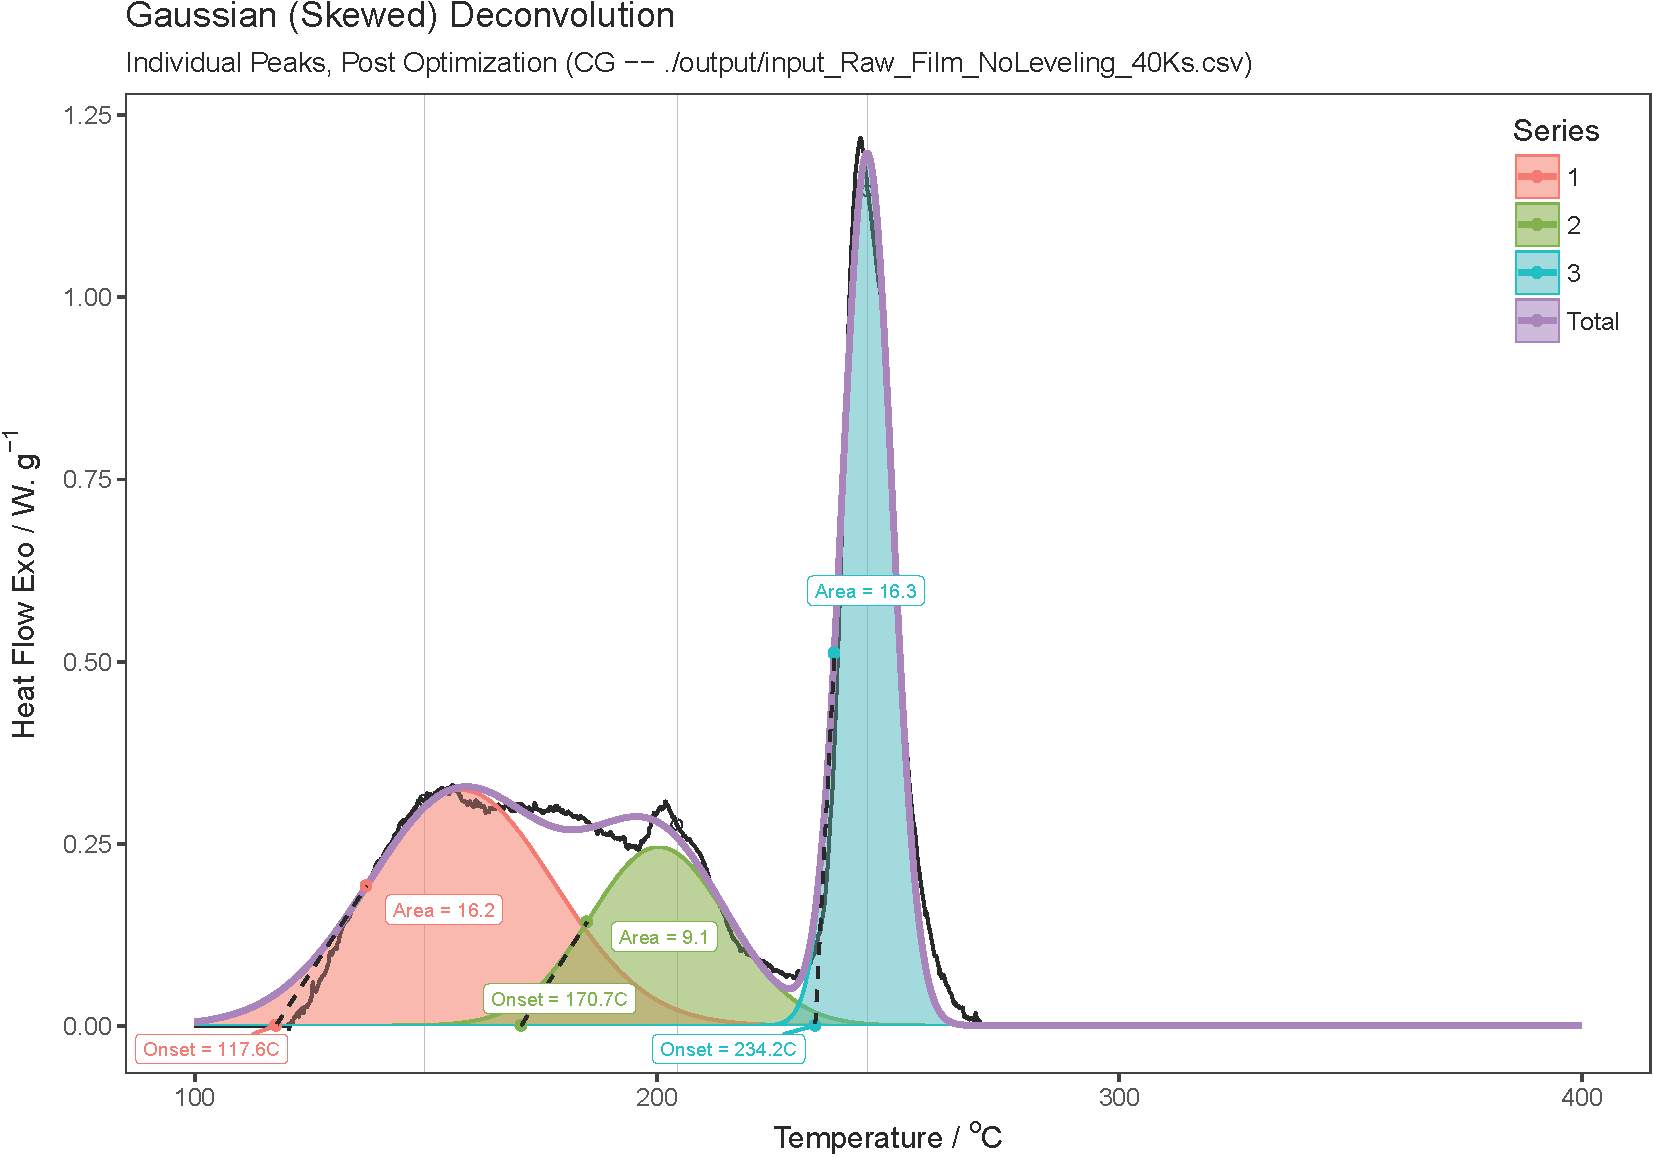
\includegraphics[width=.3\textwidth]{input_Raw_Film_NoLeveling_40Ks_result_A5lsc.png}\quad
	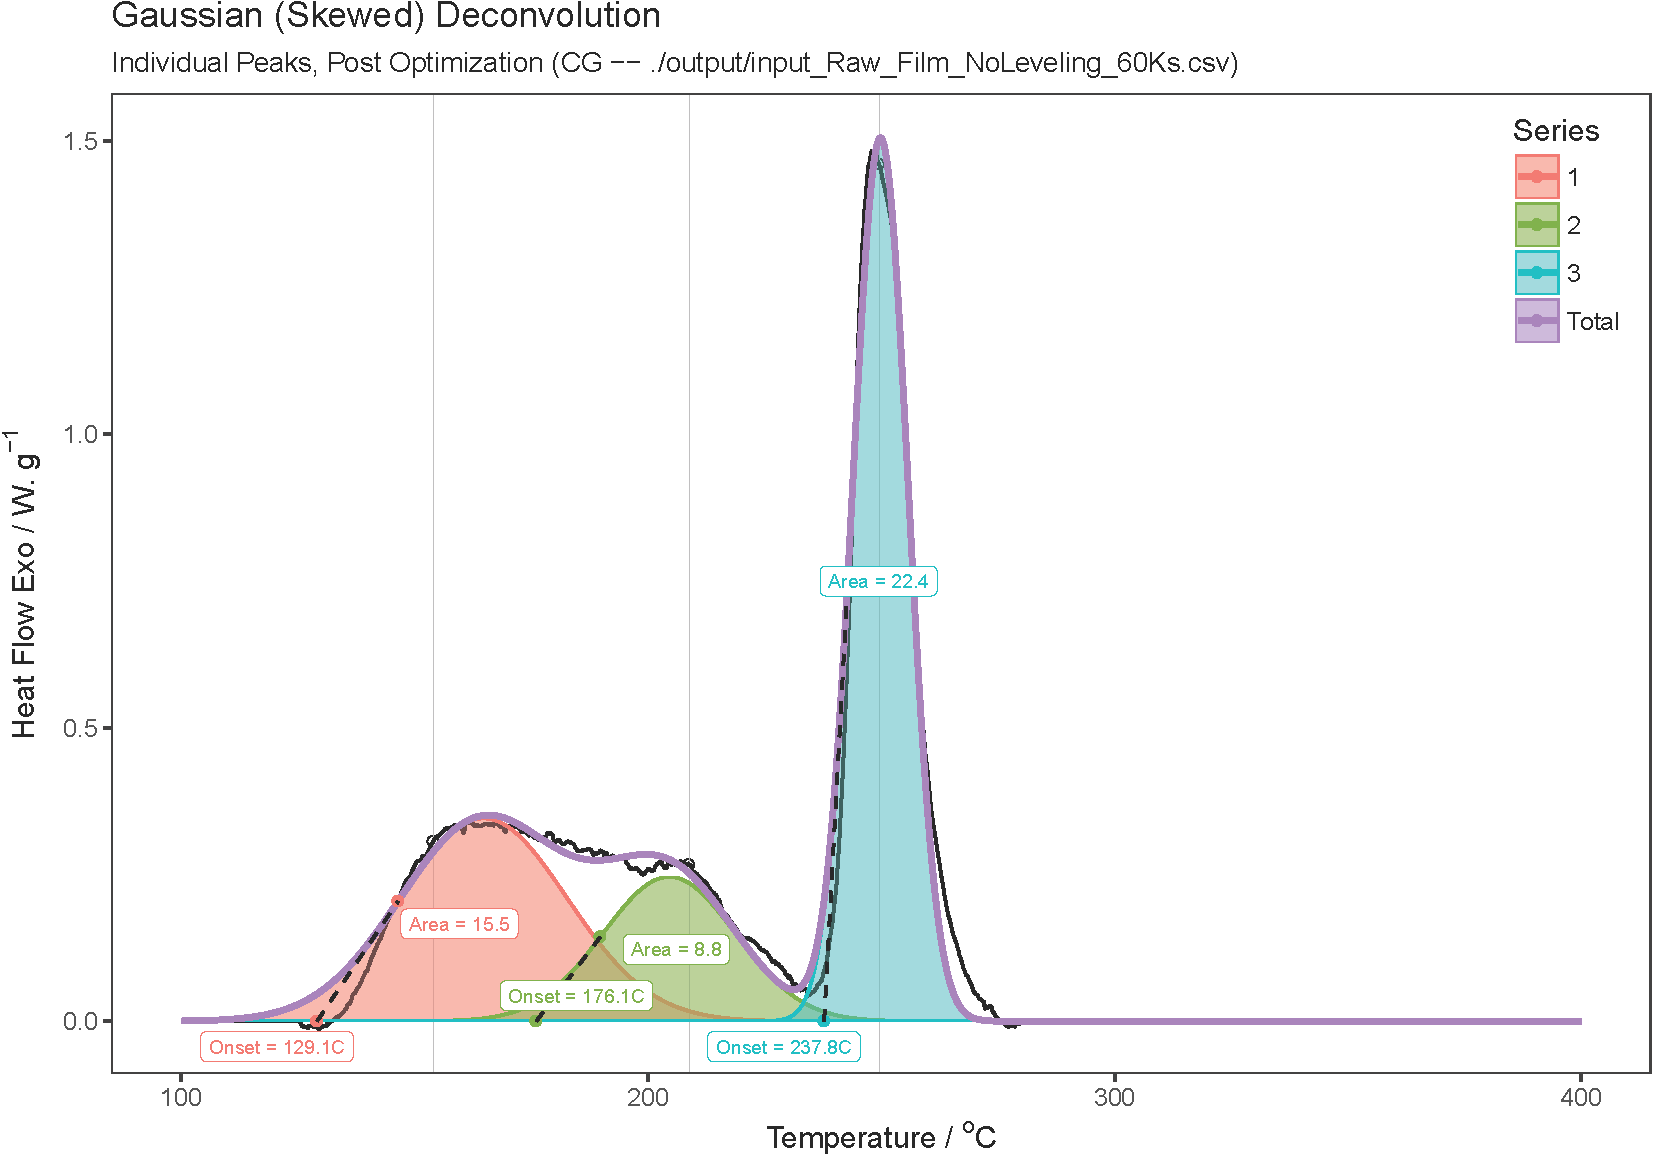
\includegraphics[width=.3\textwidth]{input_Raw_Film_NoLeveling_60Ks_result_A5lsc.png}\quad
	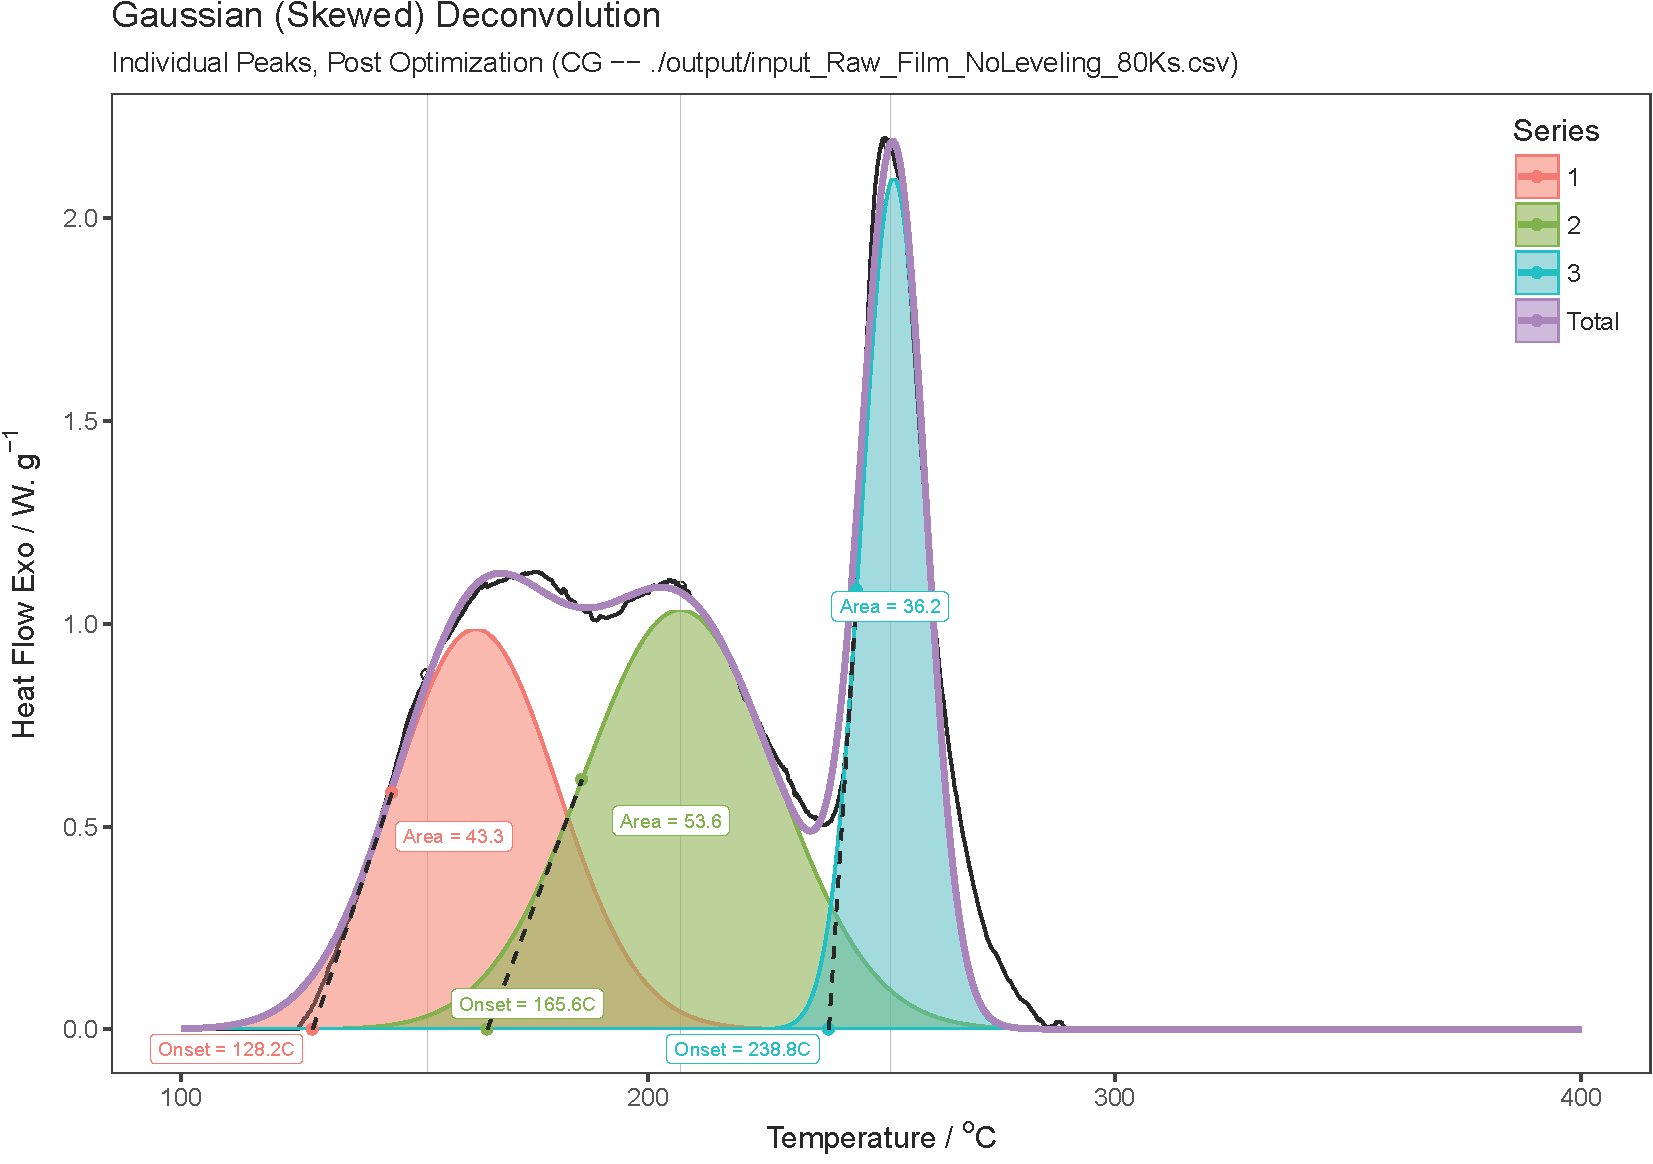
\includegraphics[width=.3\textwidth]{input_Raw_Film_NoLeveling_80Ks_result_A5lsc.png}
	\medskip
	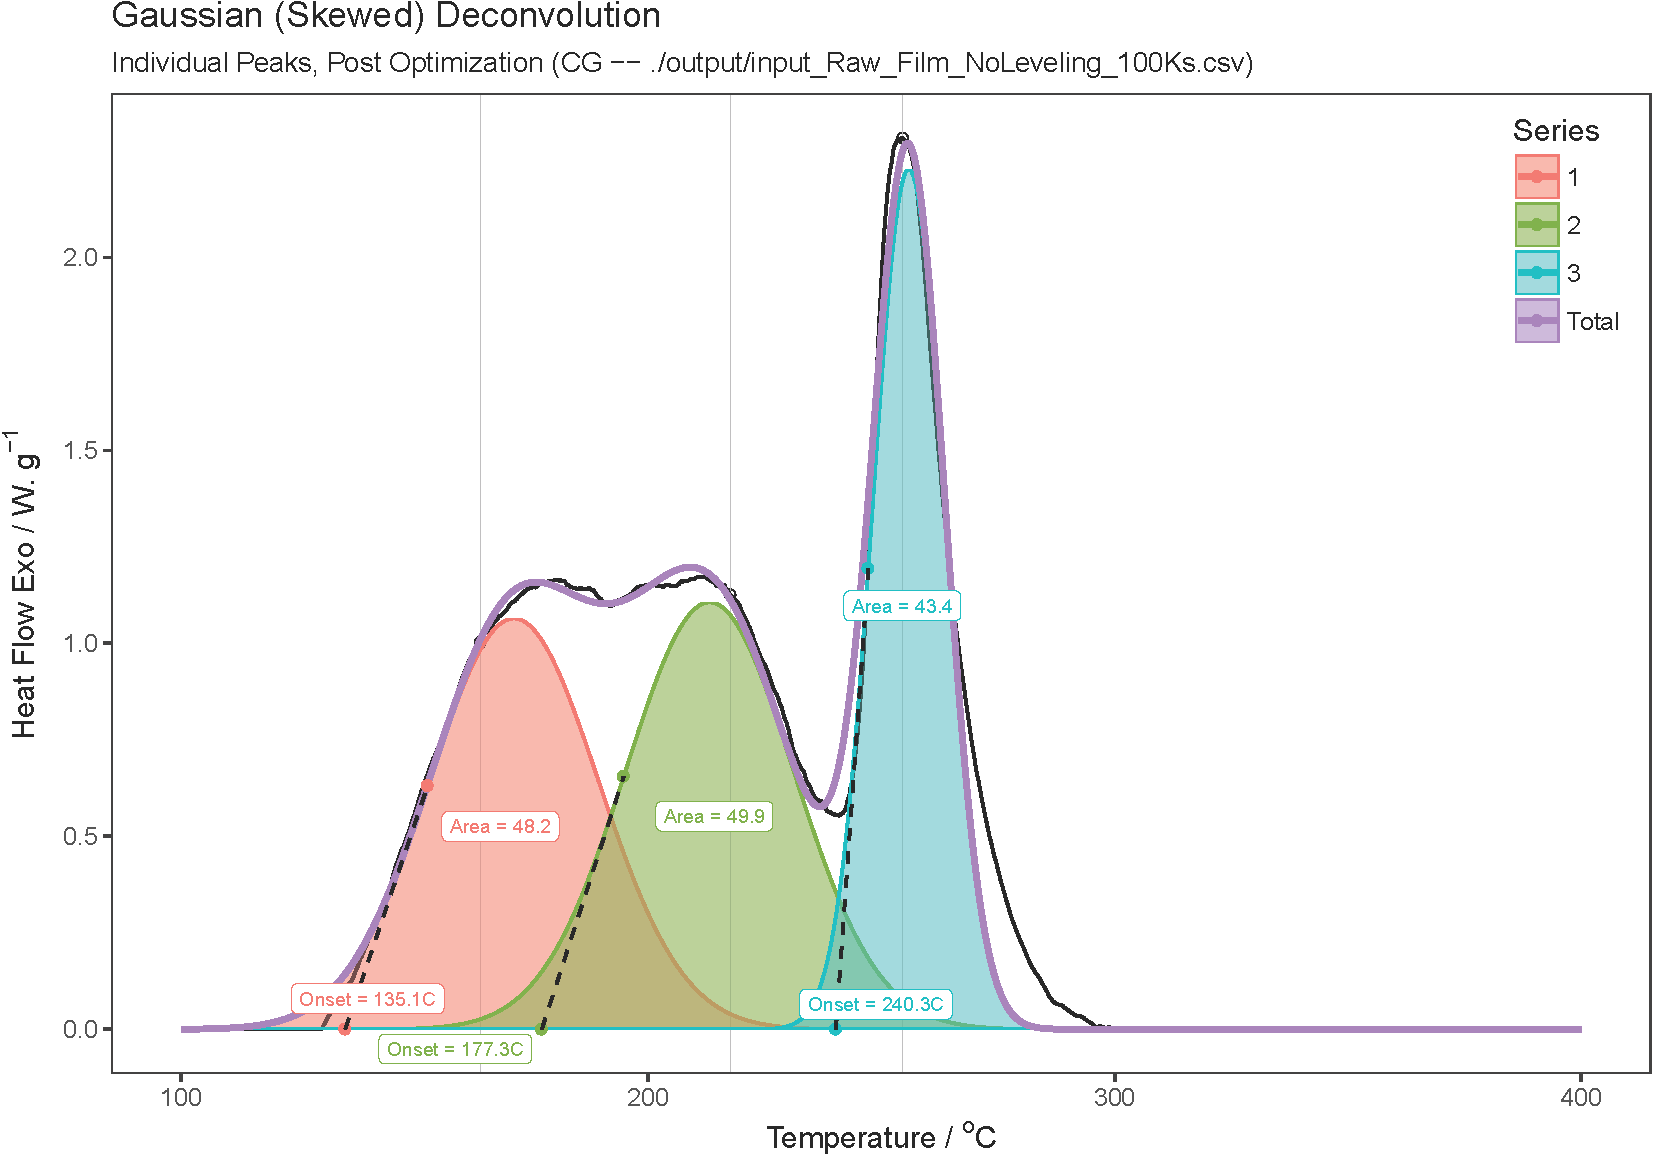
\includegraphics[width=.3\textwidth]{input_Raw_Film_NoLeveling_100Ks_result_A5lsc.png}
	\caption{\acrshort{dsc} deconvolution for the film. From left to right, top to bottom, 15, 20, 30, 40, 60, 80, 100 K/min.}
	\label{fig:DSC_Film_Decon}
\end{figure}

\subsubsection{Onset determination}

Numerical solutions were used to deconvolute the isochronic \acrshort{dsc} data so the various \Tx~ onsets could be accurately determined. This numerical fitting utilised a summation of skewed Gaussian curves to fit a target curve corresponding to the original data; as is a common method \cite{Ashour2010, Yamamoto2007, Spink2008, Spink2015, Schaffer2005}. This fitting summation takes the form of Equation \ref{equ:GaussianSummation} \todo{this is non-skewed form. It is a place holder}.

\begin{equation}
	f(x) = \sum_{n=i}^{n} h_{i}~ e^-{\bigg(\frac{(x-T_{i})^2}{(2c_{j})^2}\bigg)}
	\label{equ:GaussianSummation}
\end{equation}

Where $h$ is the enthalpy peak intensity, $T$ is the temperature at the enthalpy peak centre, and $c$ is the Gaussian RMS width.

The final converged solutions of this fitting for both the bulk and film are shown in Figures \ref{fig:DSC_Bulk_Decon} and \ref{fig:DSC_Film_Decon} respectively. These results are tabulated in Table \ref{tab:BulkOnsets} for the bulk and Table \ref{tab:FilmOnsets} for the film. Note \Tg~ and \Tx$_{1}$ are obtained from the original raw data, not the deconvolution.

\begin{table}[h]
	\centering
	\begin{tabular}{ c c c c c c c }
		\toprule
		Heating Rate \acrshort{ht} & \acrshort{Tg} & $T_{x1}$ & $T_{x2}$ & $T_{x3}$ & $T_{x4}$ & $T_{x5}$ \\ 
		$K/min$ & & & & & & \\
		\midrule
		100 & 136.1 & 164.8 & 193.4 & 201.8 & 240.2 & 262.4 \\
		80  & 132.0 & 160.0 & 194.4 & 201.9 & 238.2 & 260.3 \\
		60  & 129.6 & 157.7 & 190.0 & 197.8 & 232.9 & 259.0 \\
		40  & 126.6 & 155.2 & 189.0 & 200.0 & 226.4 & 254.7 \\
		30  & 126.2 & 151.5 & 187.0 & 198.4 & 221.0 & 251.1 \\
		20  & 125.1 & 149.8 & 188.4 & 197.0 & 216.0 & 246.8 \\
		15  & 123.8 & 148.3 & 186.2 & 195.6 & 212.2 & 243.9 \\
		10  & 123.5 & 144.5 & 183.4 & 192.9 & 207.4 & 239.8 \\
		5   & 120.5 & 141.1 & 179.7 & 187.5 & 199.8 & 232.7 \\ 
		\bottomrule
	\end{tabular}
	\caption{Bulk \MgZnCa~ alloy onset temperatures for the various \acrshort{dsc} \acrlongpl{ht} \acrshort{ht}. All temperatures are in \degree C.}
	\label{tab:BulkOnsets}
\end{table}

\begin{table}[h]
	\centering
	\begin{tabular}{ c c c c c c c }
		\toprule
		Heating Rate \acrshort{ht} & \acrshort{Tg} & $T_{x1}$ & $T_{x2}$ & $T_{x3}$ & $T_{x4}$ & $T_{x5}$ \\ 
		$K/min$ & & & & & & \\
		\midrule
		100 & 108.5 & 128.6 &  & 177.3 &  & 240.3 \\
		80  & 106.0 & 121.2 &  & 165.6 &  & 238.8 \\
		60  & 107.3 & 134.0 &  & 176.1 &  & 237.8 \\
		40  & 100.2 & 119.8 &  & 170.7 &  & 234.2 \\
		30  & 95.3  & 110.4 &  & 169.5 &  & 232.5 \\
		20  & 95.5  & 115.2 &  & 170.5 &  & 229.4 \\
		15  & 92.5  & 113.5 &  & 168.8 &  & 224.0 \\
		\bottomrule
	\end{tabular}
	\caption{Film \MgZnCa~ alloy onset temperatures for the various \acrshort{dsc} \acrlongpl{ht} \acrshort{ht}. All temperatures are in \degree C.}
	\label{tab:FilmOnsets}
\end{table}

%single image
\begin{figure}[b]
	\centering
	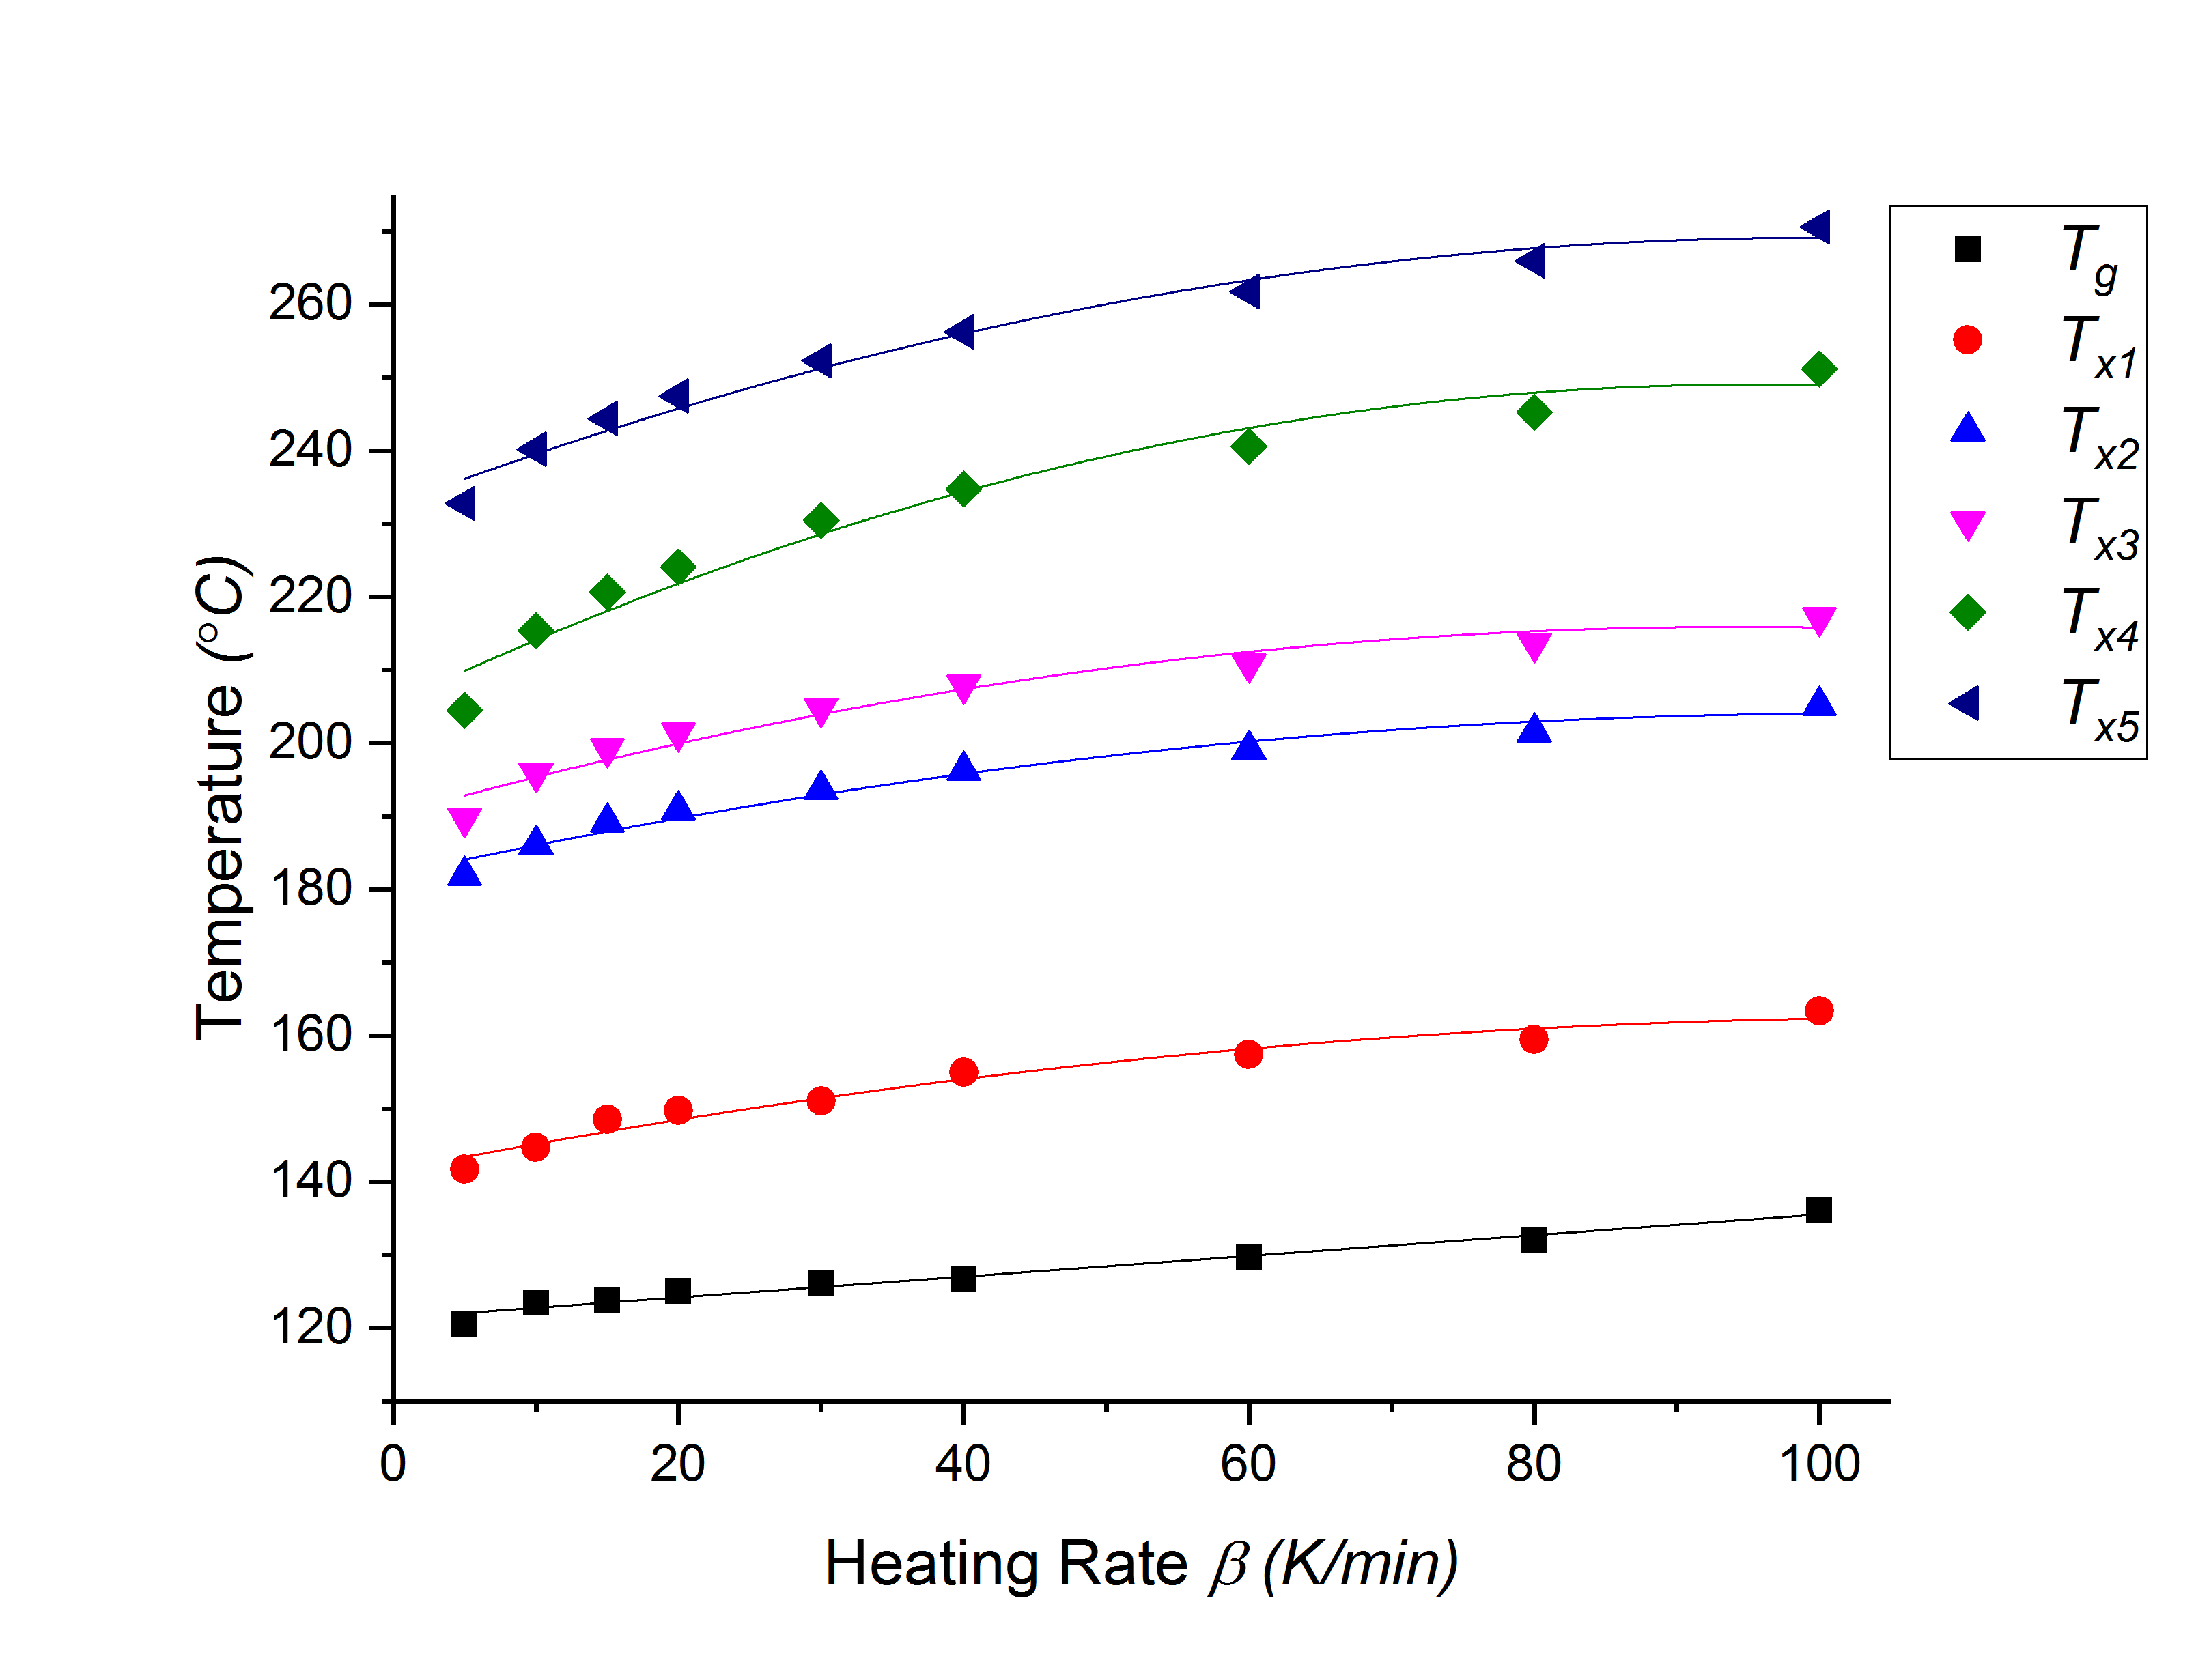
\includegraphics[width=0.55\textwidth]{Bulk_Onset_Peaks_Relaxed_120C.png}
	\caption[Table of contents Capition]{The \Tg s and \Tx es of the bulk \MgZnCa~ at all heating rates. }%global caption
	\label{fig:DSC_Onsets_Bulk}
\end{figure}

%single image
\begin{figure}[b]
	\centering
	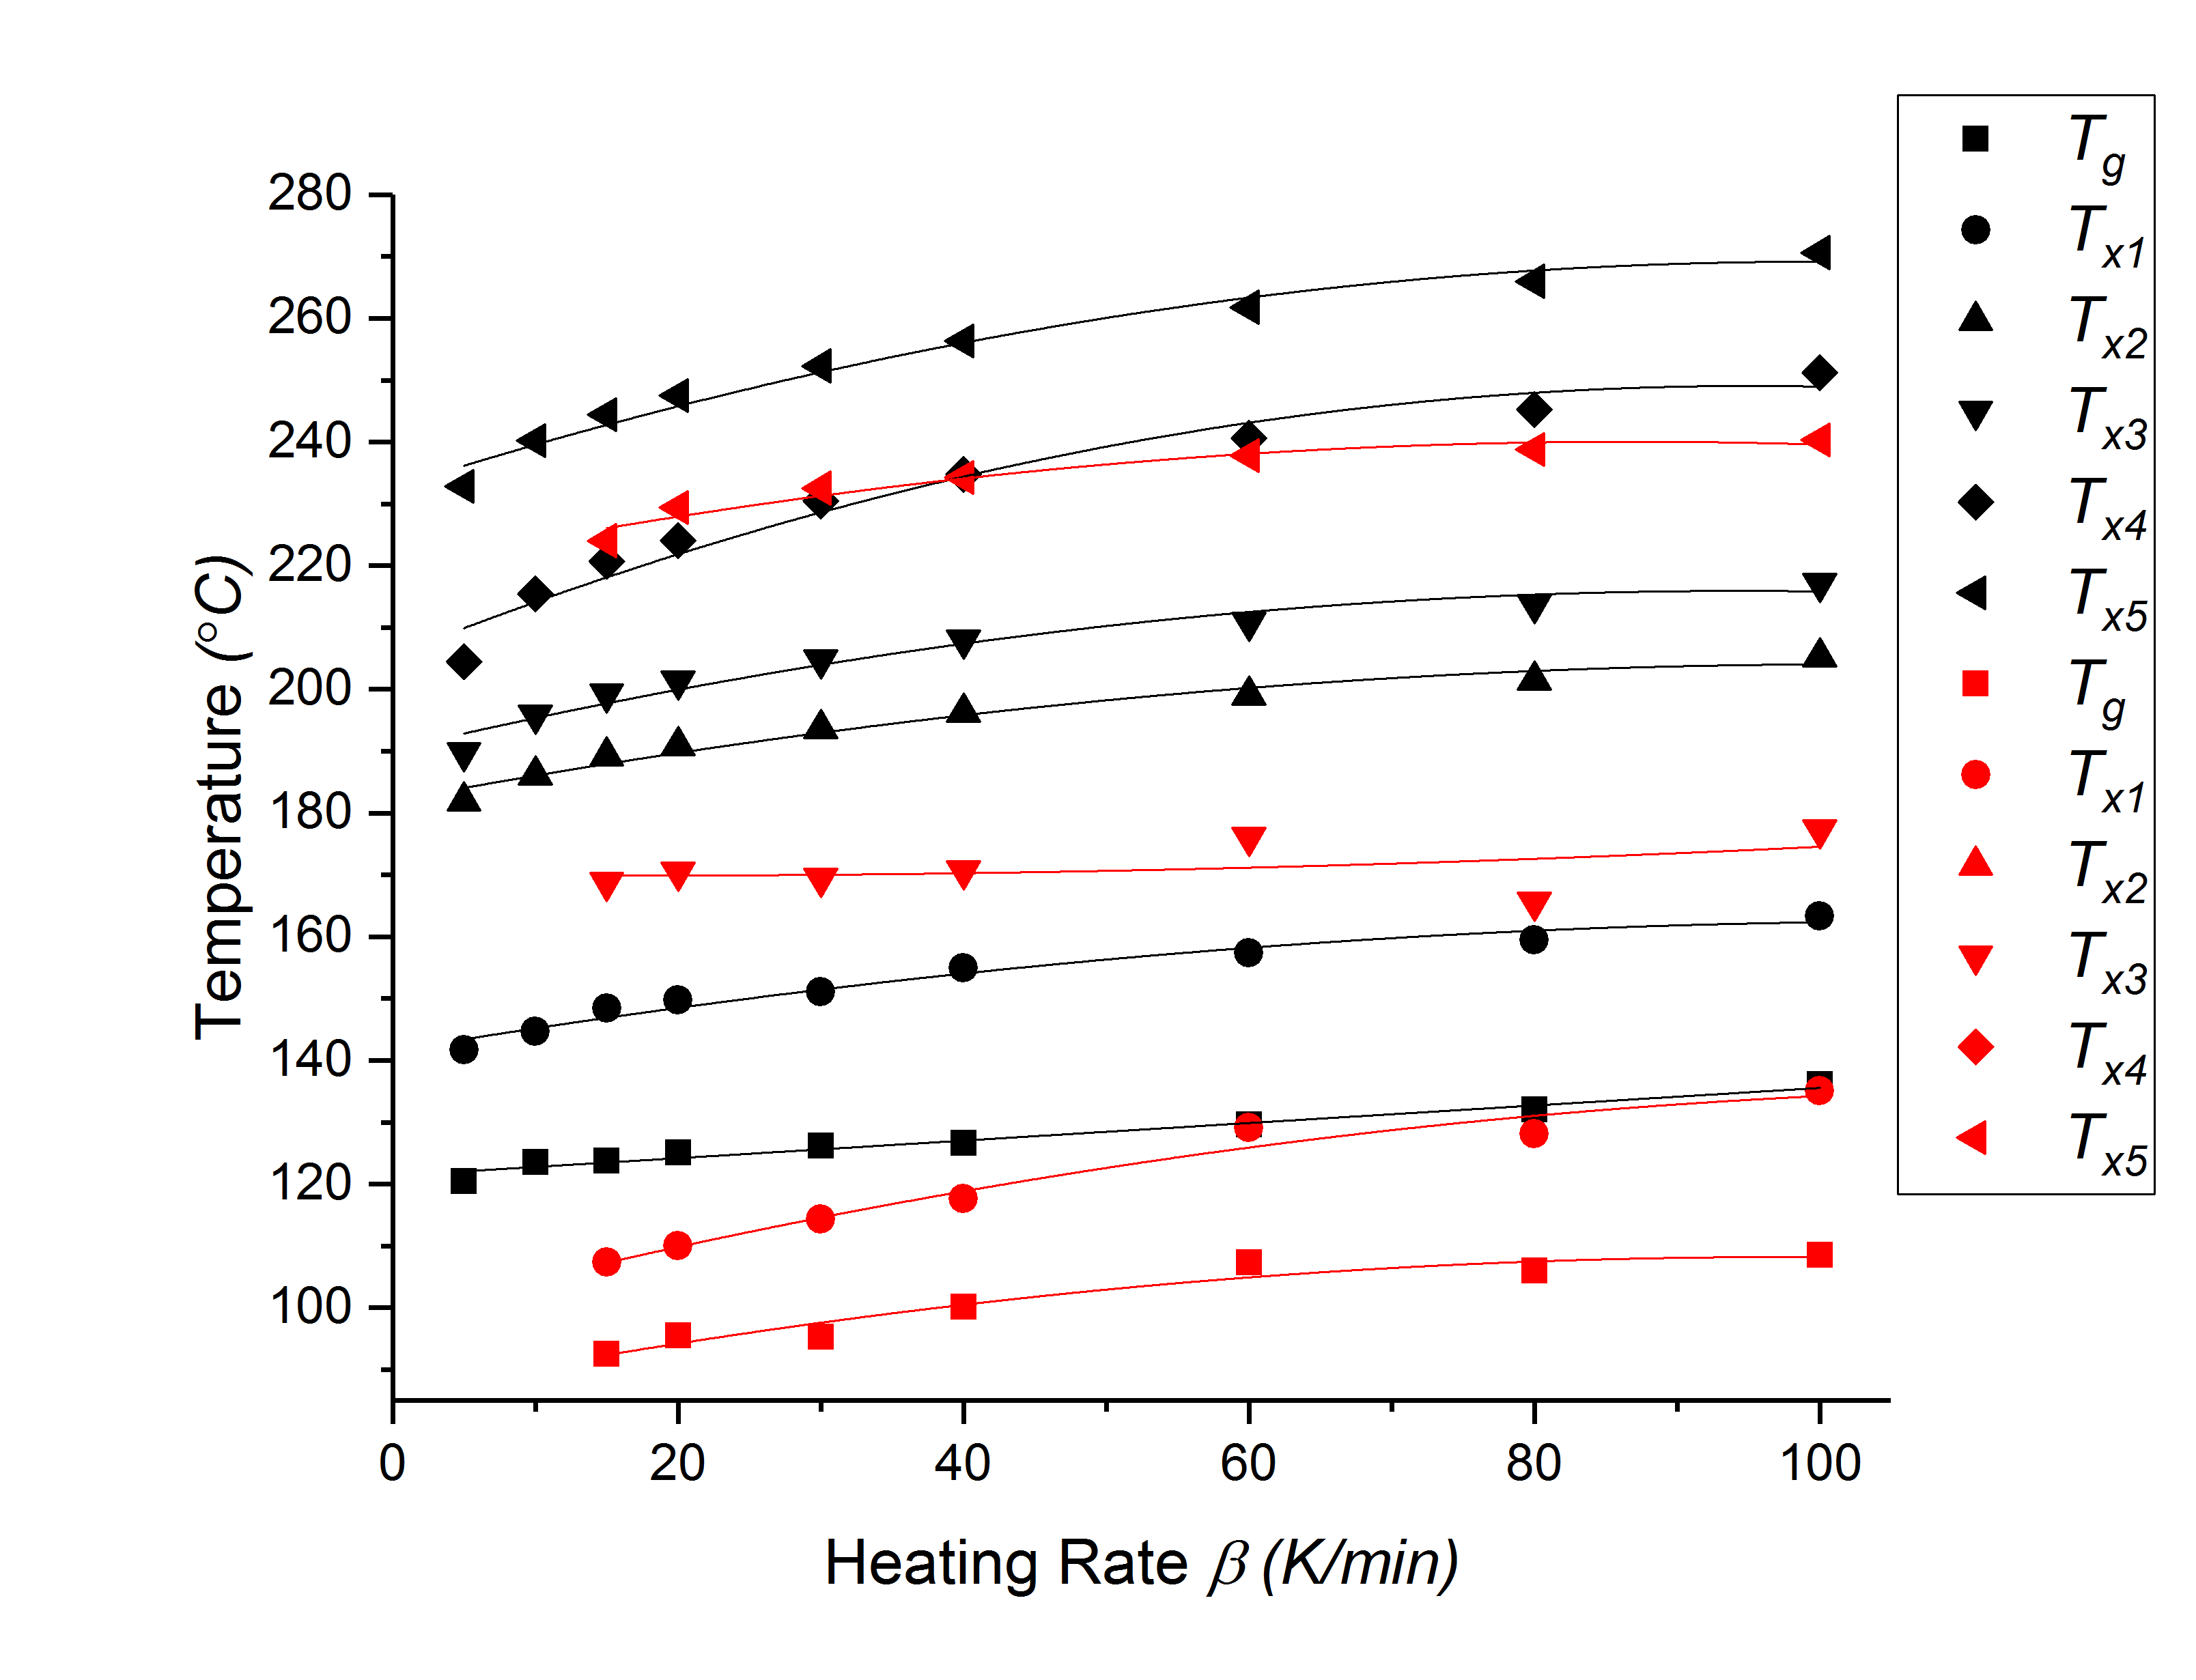
\includegraphics[width=0.55\textwidth]{Onsets_BulkandFilm.png}
	\caption[Table of contents Capition]{The \Tg s and \Tx es of the bulk and film \MgZnCa~ at all heating rates. }%global caption
	\label{fig:DSC_Onsets_BulkFilm}
\end{figure}

\subsubsection{Reaction enthalpy}


Target error plot? 

\begin{table}[h]
	\centering
	\begin{tabular}{ c c c c c c }
		\toprule
		Heating Rate \acrshort{ht} & $h_{T_{x1}}$ & $h_{T_{x2}}$ & $h_{T_{x3}}$ & $h_{T_{x4}}$ & $h_{T_{x5}}$ \\ 
		$K/min$ & $J/g$ & $J/g$ & $J/g$ & $J/g$ & $J/g$ \\
		\midrule
		100  & 59.59 & 6.97 & 49.16 & 22.84 & 46.08 \\
		80   & 42.61 & 6.08 & 32.33 & 18.27 & 31.25 \\
		60   & 30.02 & 4.05 & 25.41 & 16.76 & 19.81 \\
		40   & 16.93 & 4.36 & 12.44 & 11.13 & 11.68 \\
		30   & 12.03 & 3.68 & 9.32  & 9.18  & 9.02  \\
		20   & 7.18  & 2.21 & 4.99  & 5.67  & 5.78  \\
		15   & 5.48  & 2.01 & 3.65  & 4.69  & 4.43  \\
		10   & 3.45  & 1.43 & 2.28  & 3.14  & 2.92  \\
		5    & 1.65  & 0.69 & 1.09  & 1.47  & 1.42  \\
		\bottomrule
	\end{tabular}
	\caption{Bulk \MgZnCa~ alloy \gls{h} of crystallisation for $Tx_{1-5}$ for the various \acrshort{dsc} \acrlongpl{ht} \acrshort{ht}; \gls{h} is in $J/g$.}
	\label{tab:Bulk_Enthalpy}
\end{table}

\begin{table}[h]
	\centering
	\begin{tabular}{ c c c c c c }
		\toprule
		Heating Rate \acrshort{ht} & $h_{T_{x1}}$ & $h_{T_{x2}}$ & $h_{T_{x3}}$ & $h_{T_{x4}}$ & $h_{T_{x5}}$ \\ 
		$K/min$ & $J/g$ & $J/g$ & $J/g$ & $J/g$ & $J/g$ \\
		\midrule
		100  & 48.24 &    & 49.85 &    & 43.38 \\
		80   & 43.27 &    & 53.56 &    & 36.18 \\
		60   & 15.5  &    & 8.78  &    & 22.4  \\
		40   & 16.22 &    & 9.13  &    & 16.27 \\
		30   & 13.72 &    & 7.16  &    & 11.81 \\
		20   & 6.16  &    & 2.3   &    & 7.45  \\
		15   & 6.99  &    & 3.66  &    & 6.57  \\
		\bottomrule
	\end{tabular}
	\caption{Film \MgZnCa~ alloy \gls{h} of crystallisation for $Tx_{1-5}$ for the various \acrshort{dsc} \acrlongpl{ht} \acrshort{ht}; \gls{h} is in $J/g$.}
	\label{tab:Film_Enthalpy}
\end{table}

%MultiFigure
\begin{figure}[b]
	\centering
	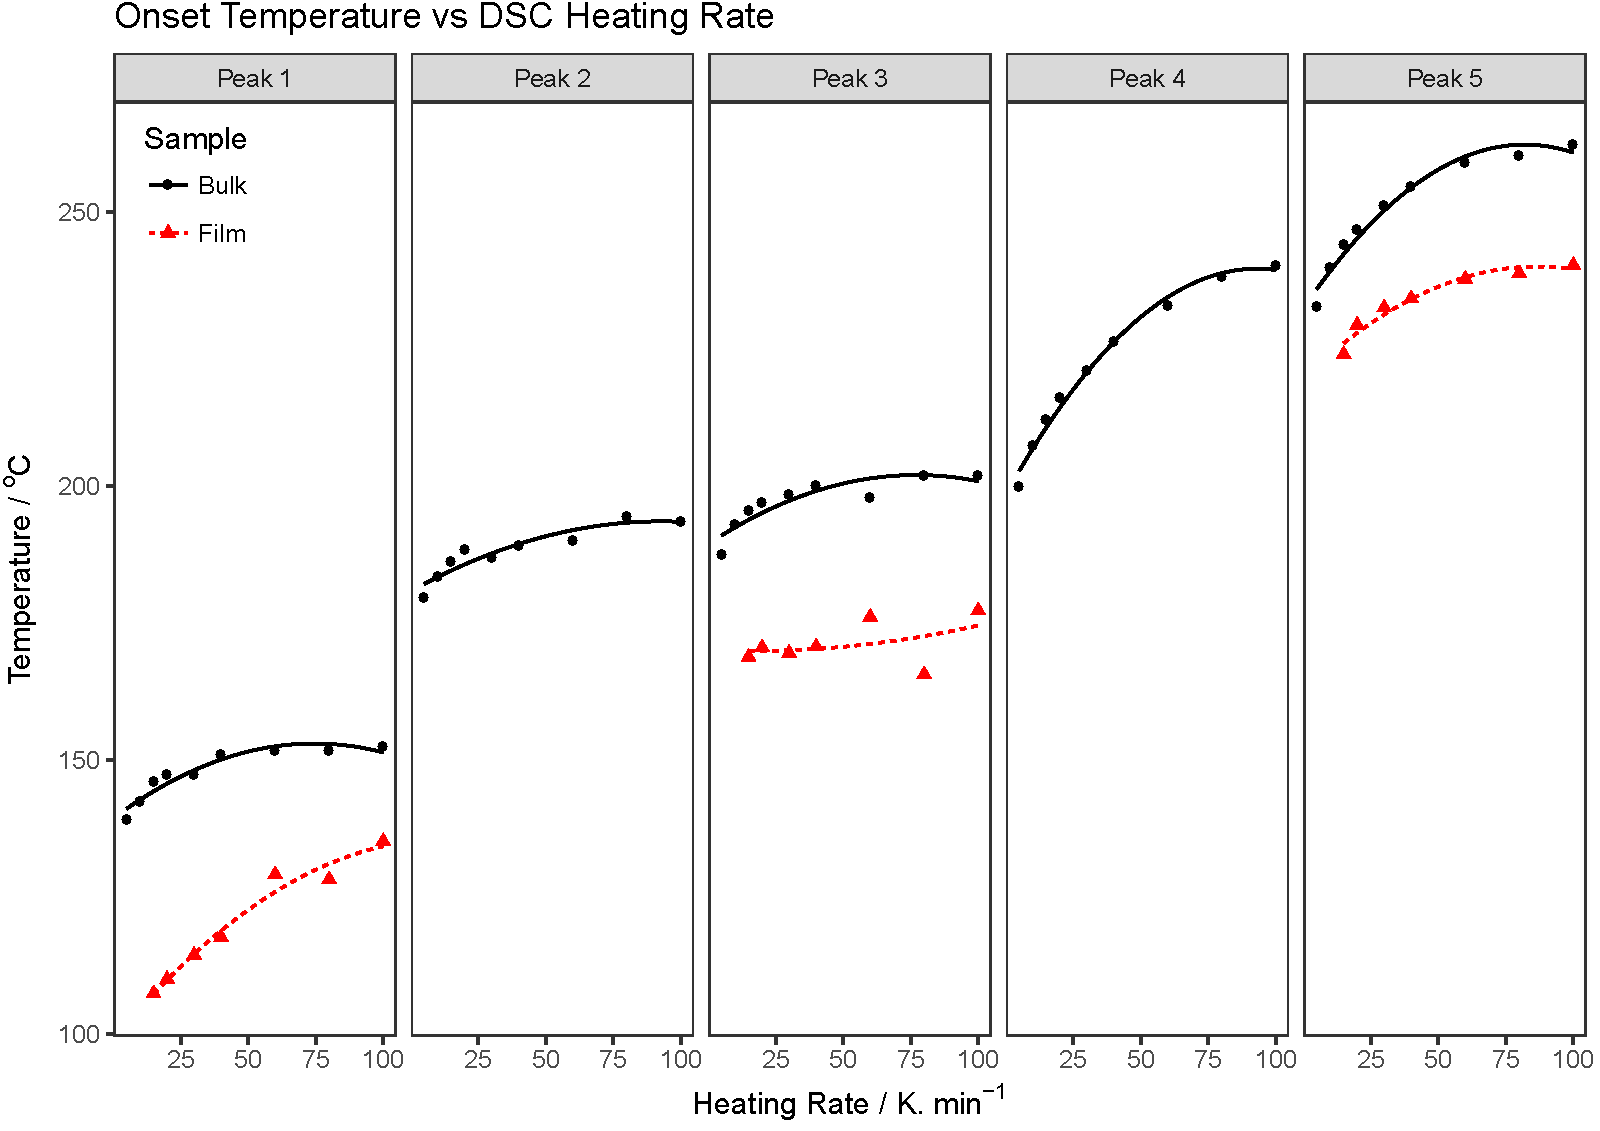
\includegraphics[width=.6\textwidth]{Decon_Onsets_BR.png}
	\medskip
	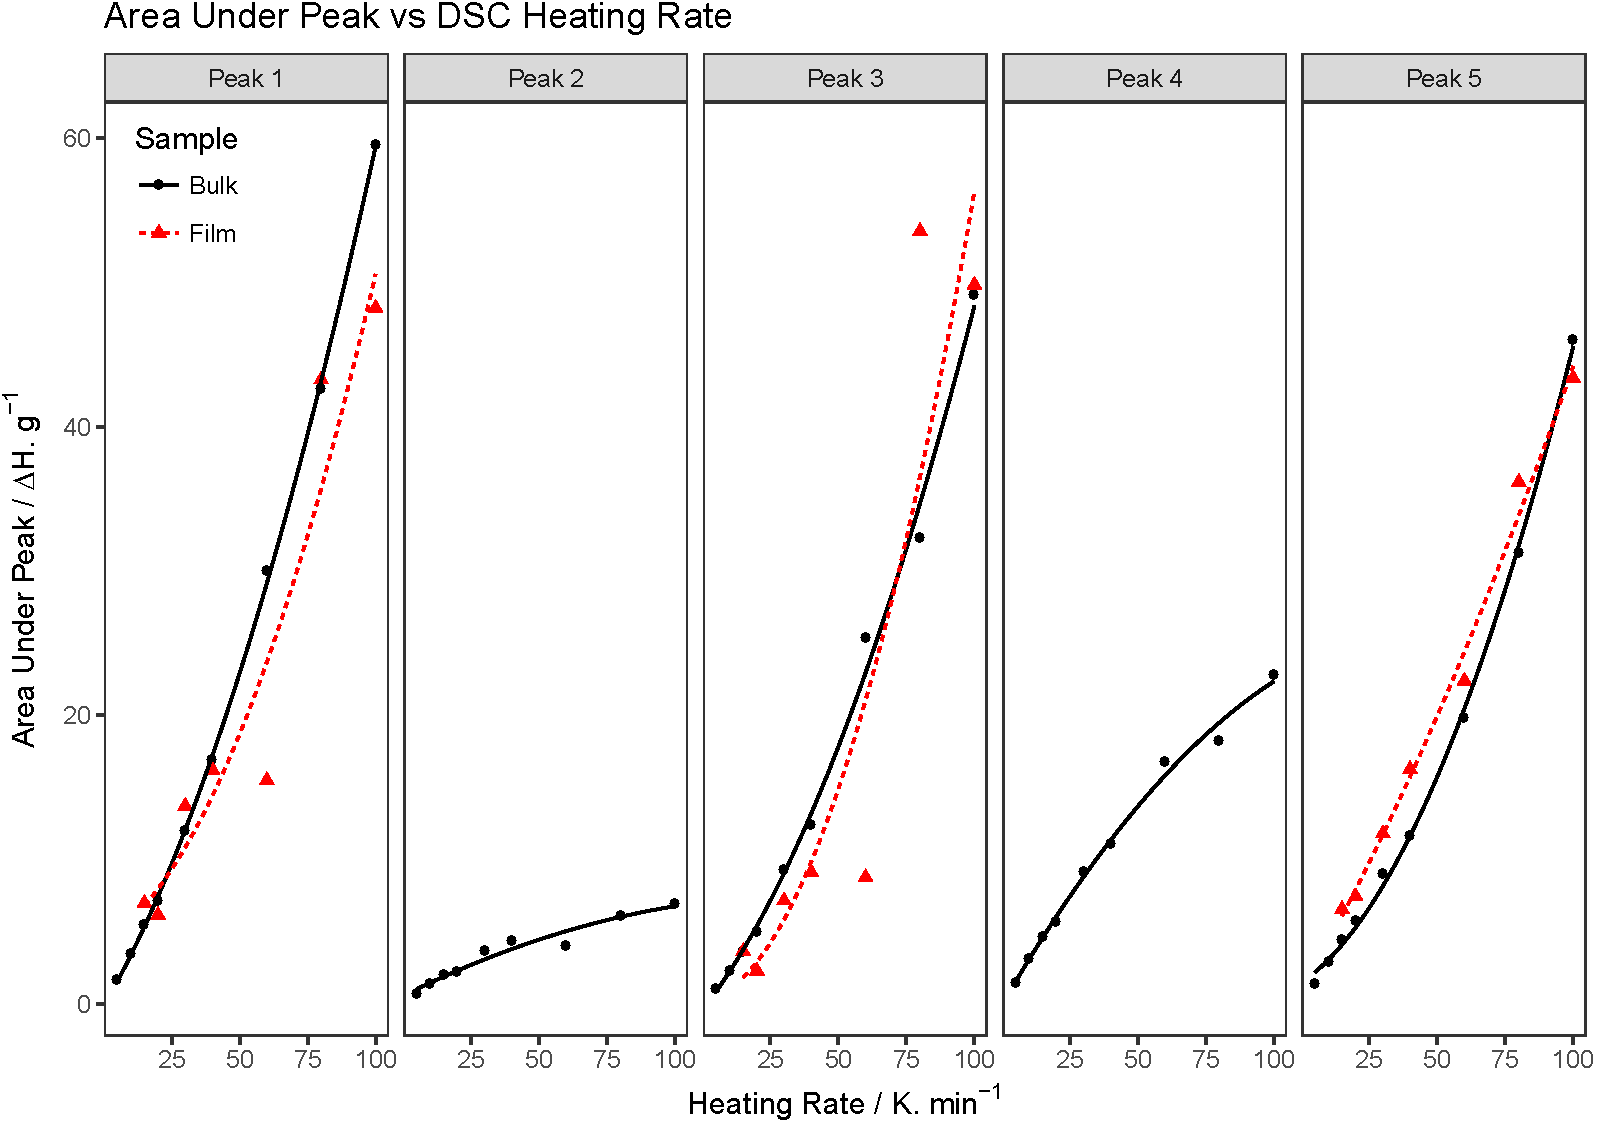
\includegraphics[width=.6\textwidth]{Decon_peak_area_BR.png}
	\caption{\acrshort{dsc} onset temperatures and enthalpy of formation for the bulk and film.}
	\label{fig:DSC_Decon}
\end{figure}

\subsubsection{Relaxation enthalpy}

\subsection{\acrshort{xrd}}
\subsubsection{Annealing \acrshort{xrd}}

Note: Key XRD sources for \MgZnCa crystallisation phase identification \cite{Zhang2013, Zhang2012, Zhang2011} 

%single image
\begin{figure}[b]
	\centering
	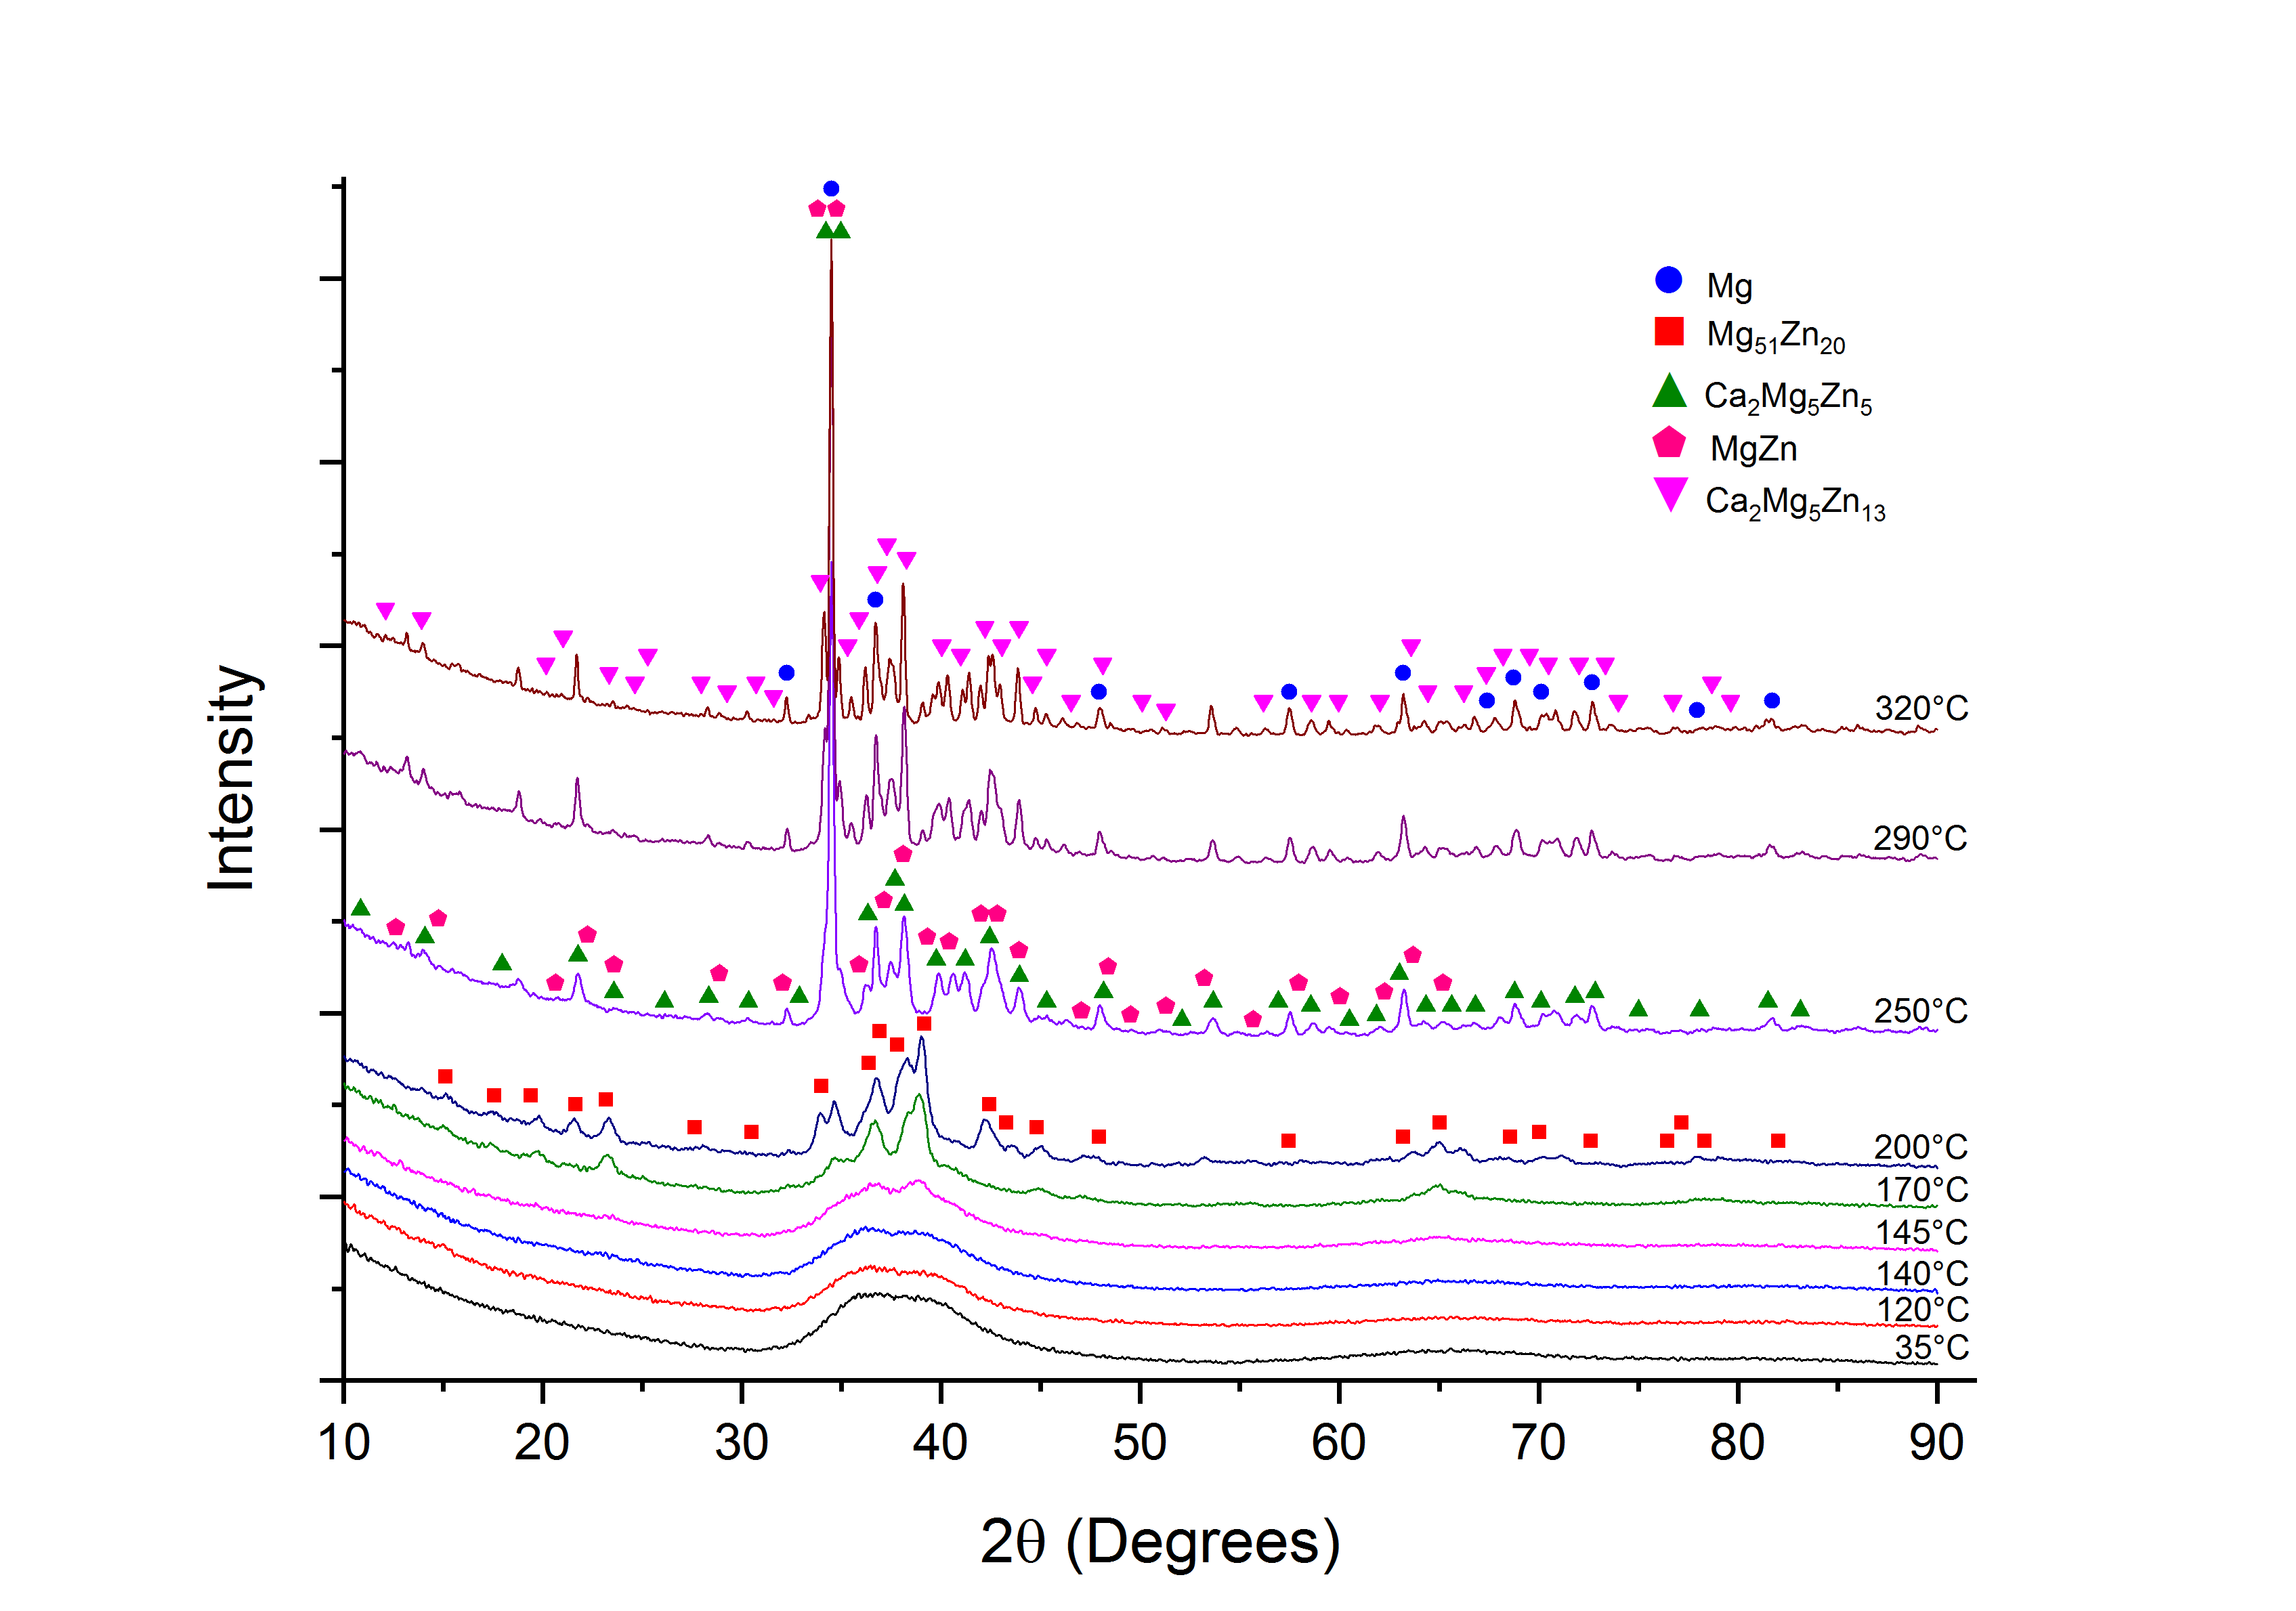
\includegraphics[width=0.9\textwidth]{XRD_Annealing_Bulk.png}
	\caption[Table of contents Capition]{\acrshort{xrd} pattern for Bulk \MgZnCa~ heated through several crystallization peaks identified from \acrshort{dsc}}
	\label{fig:XRD_Annealing_Bulk}
\end{figure}

%single image
\begin{figure}[b]
	\centering
	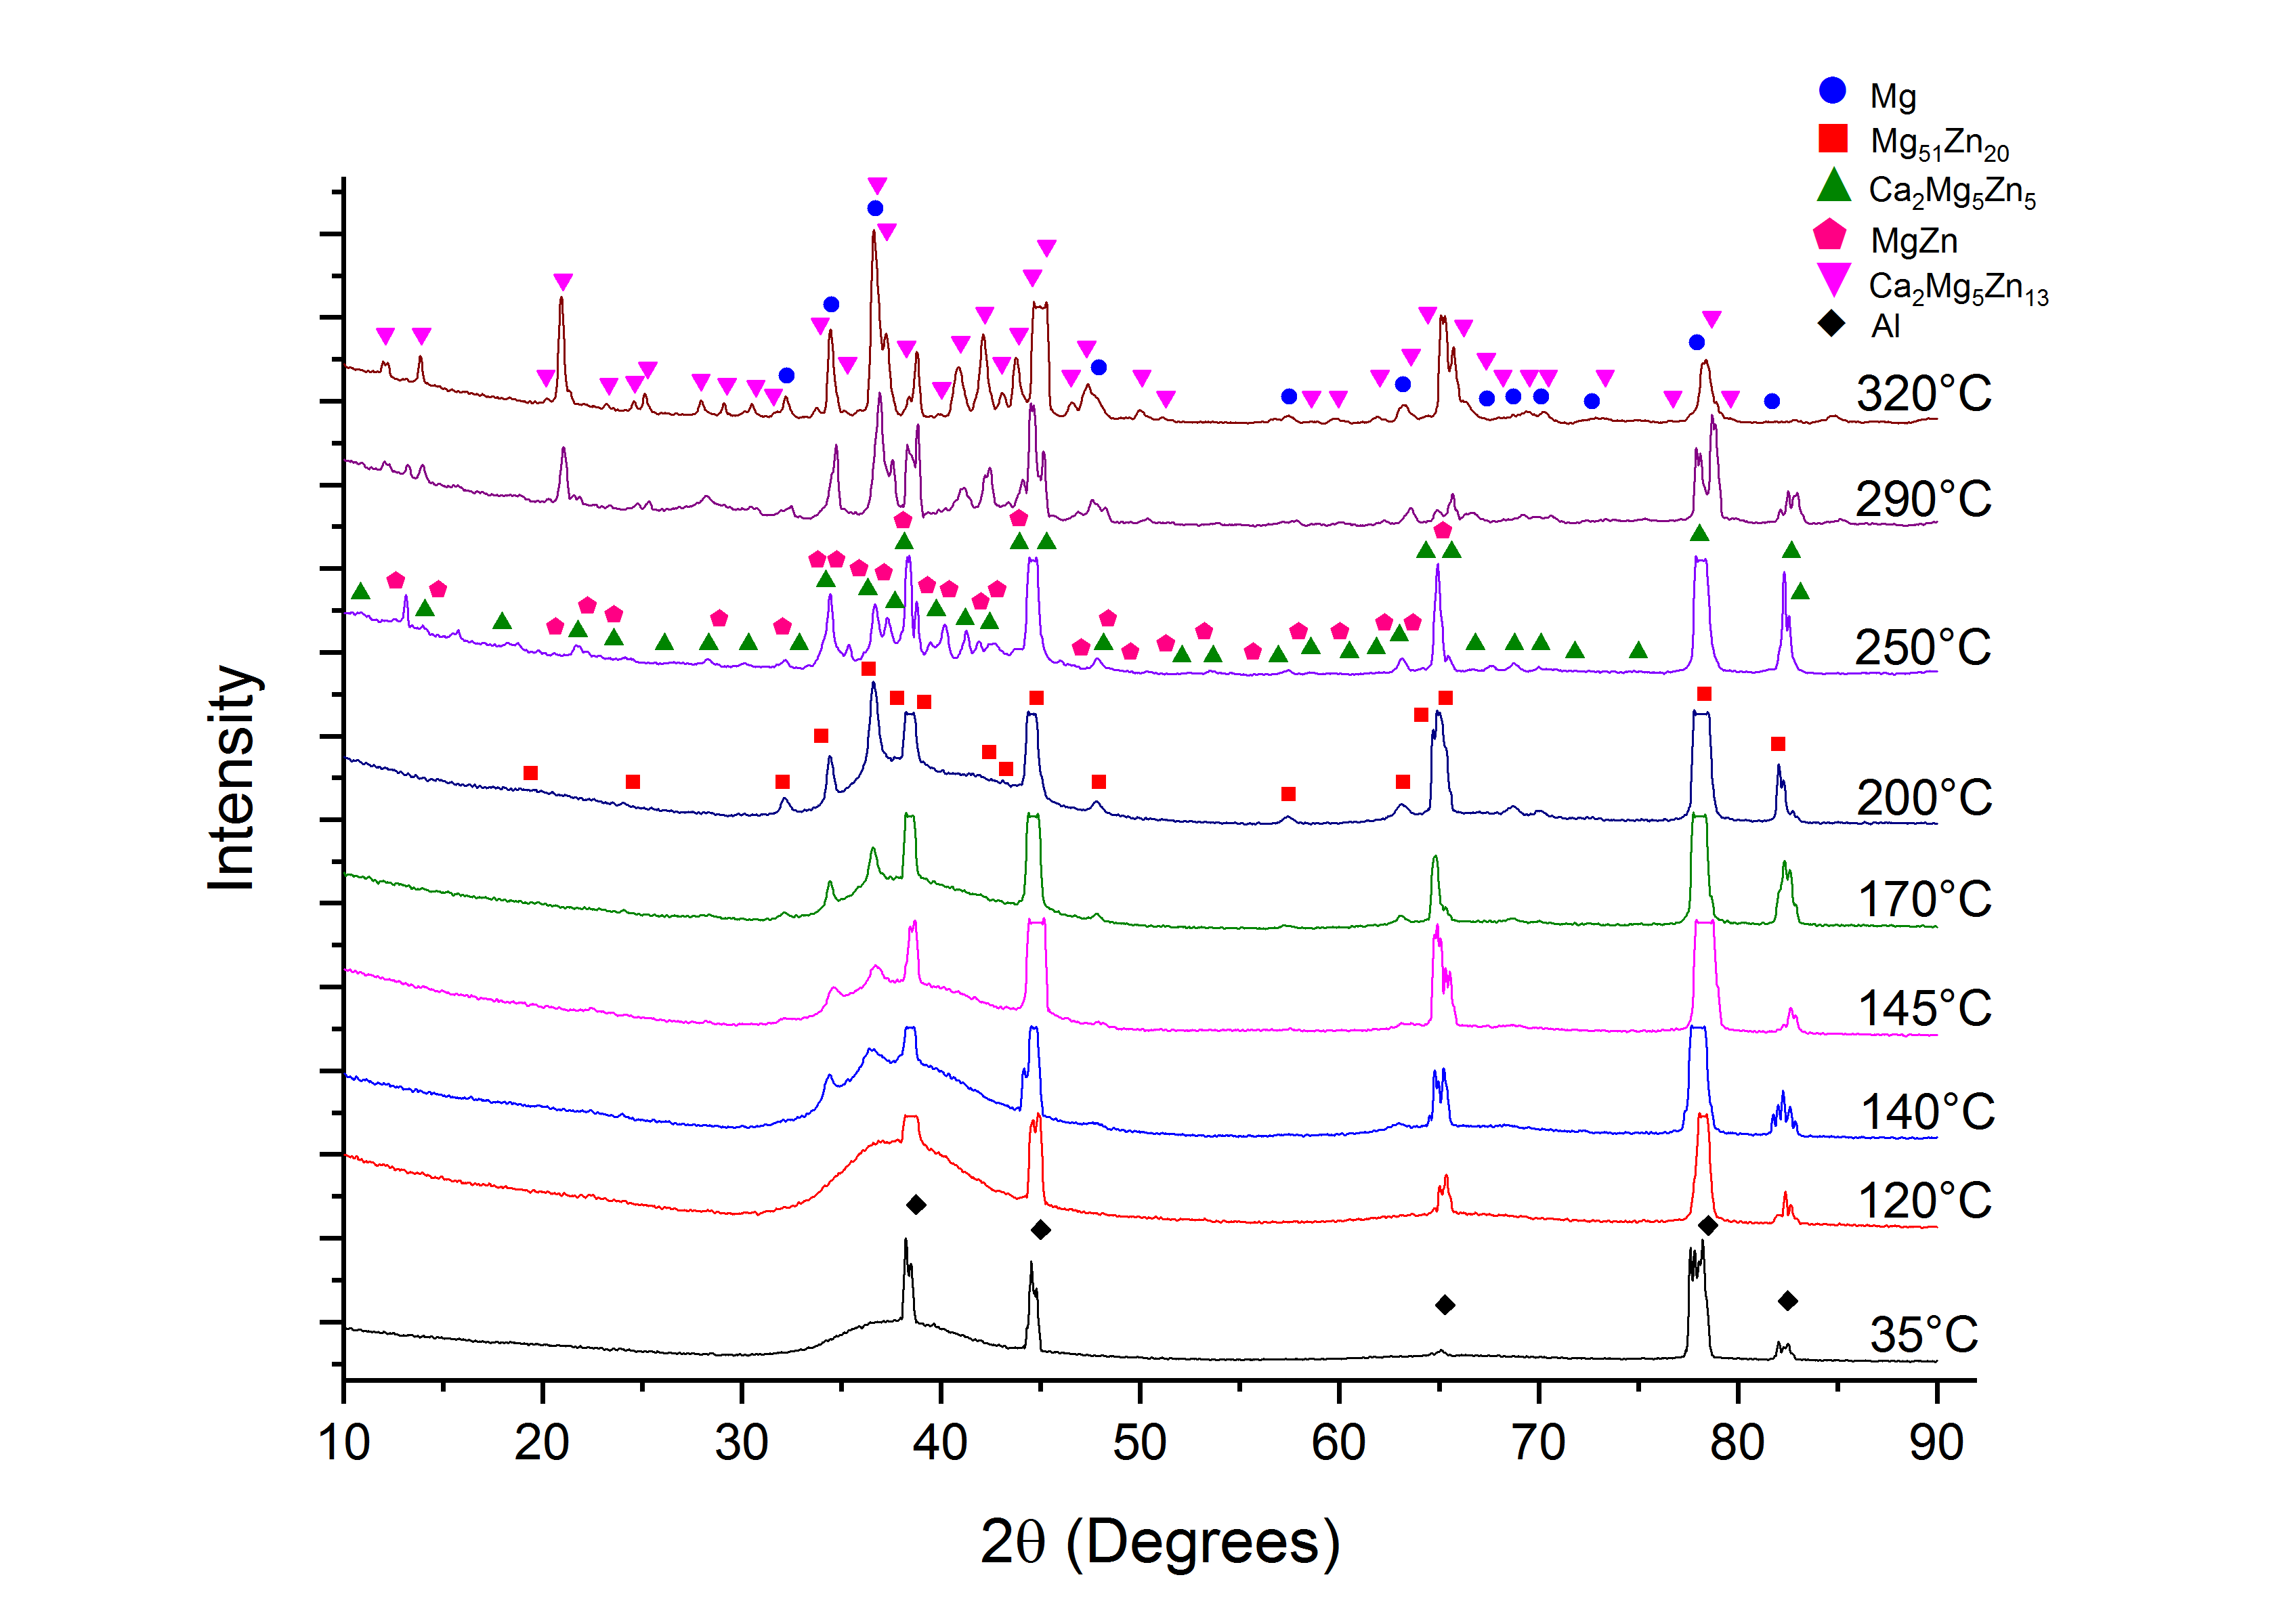
\includegraphics[width=0.9\textwidth]{XRD_Annealing_Film.png}
	\caption[Table of contents Capition]{\acrshort{xrd} pattern for Film \MgZnCa~ heated through several crystallization peaks identified from \acrshort{dsc}}
	\label{fig:XRD_Annealing_Film}
\end{figure}

\subsubsection{Dynamic \acrshort{xrd}}

%code to put 2 images side by side in a figure
\begin{figure}[b]
	\centering
	%Image 1
	\begin{subfigure}[htbp]{0.75\textwidth}
		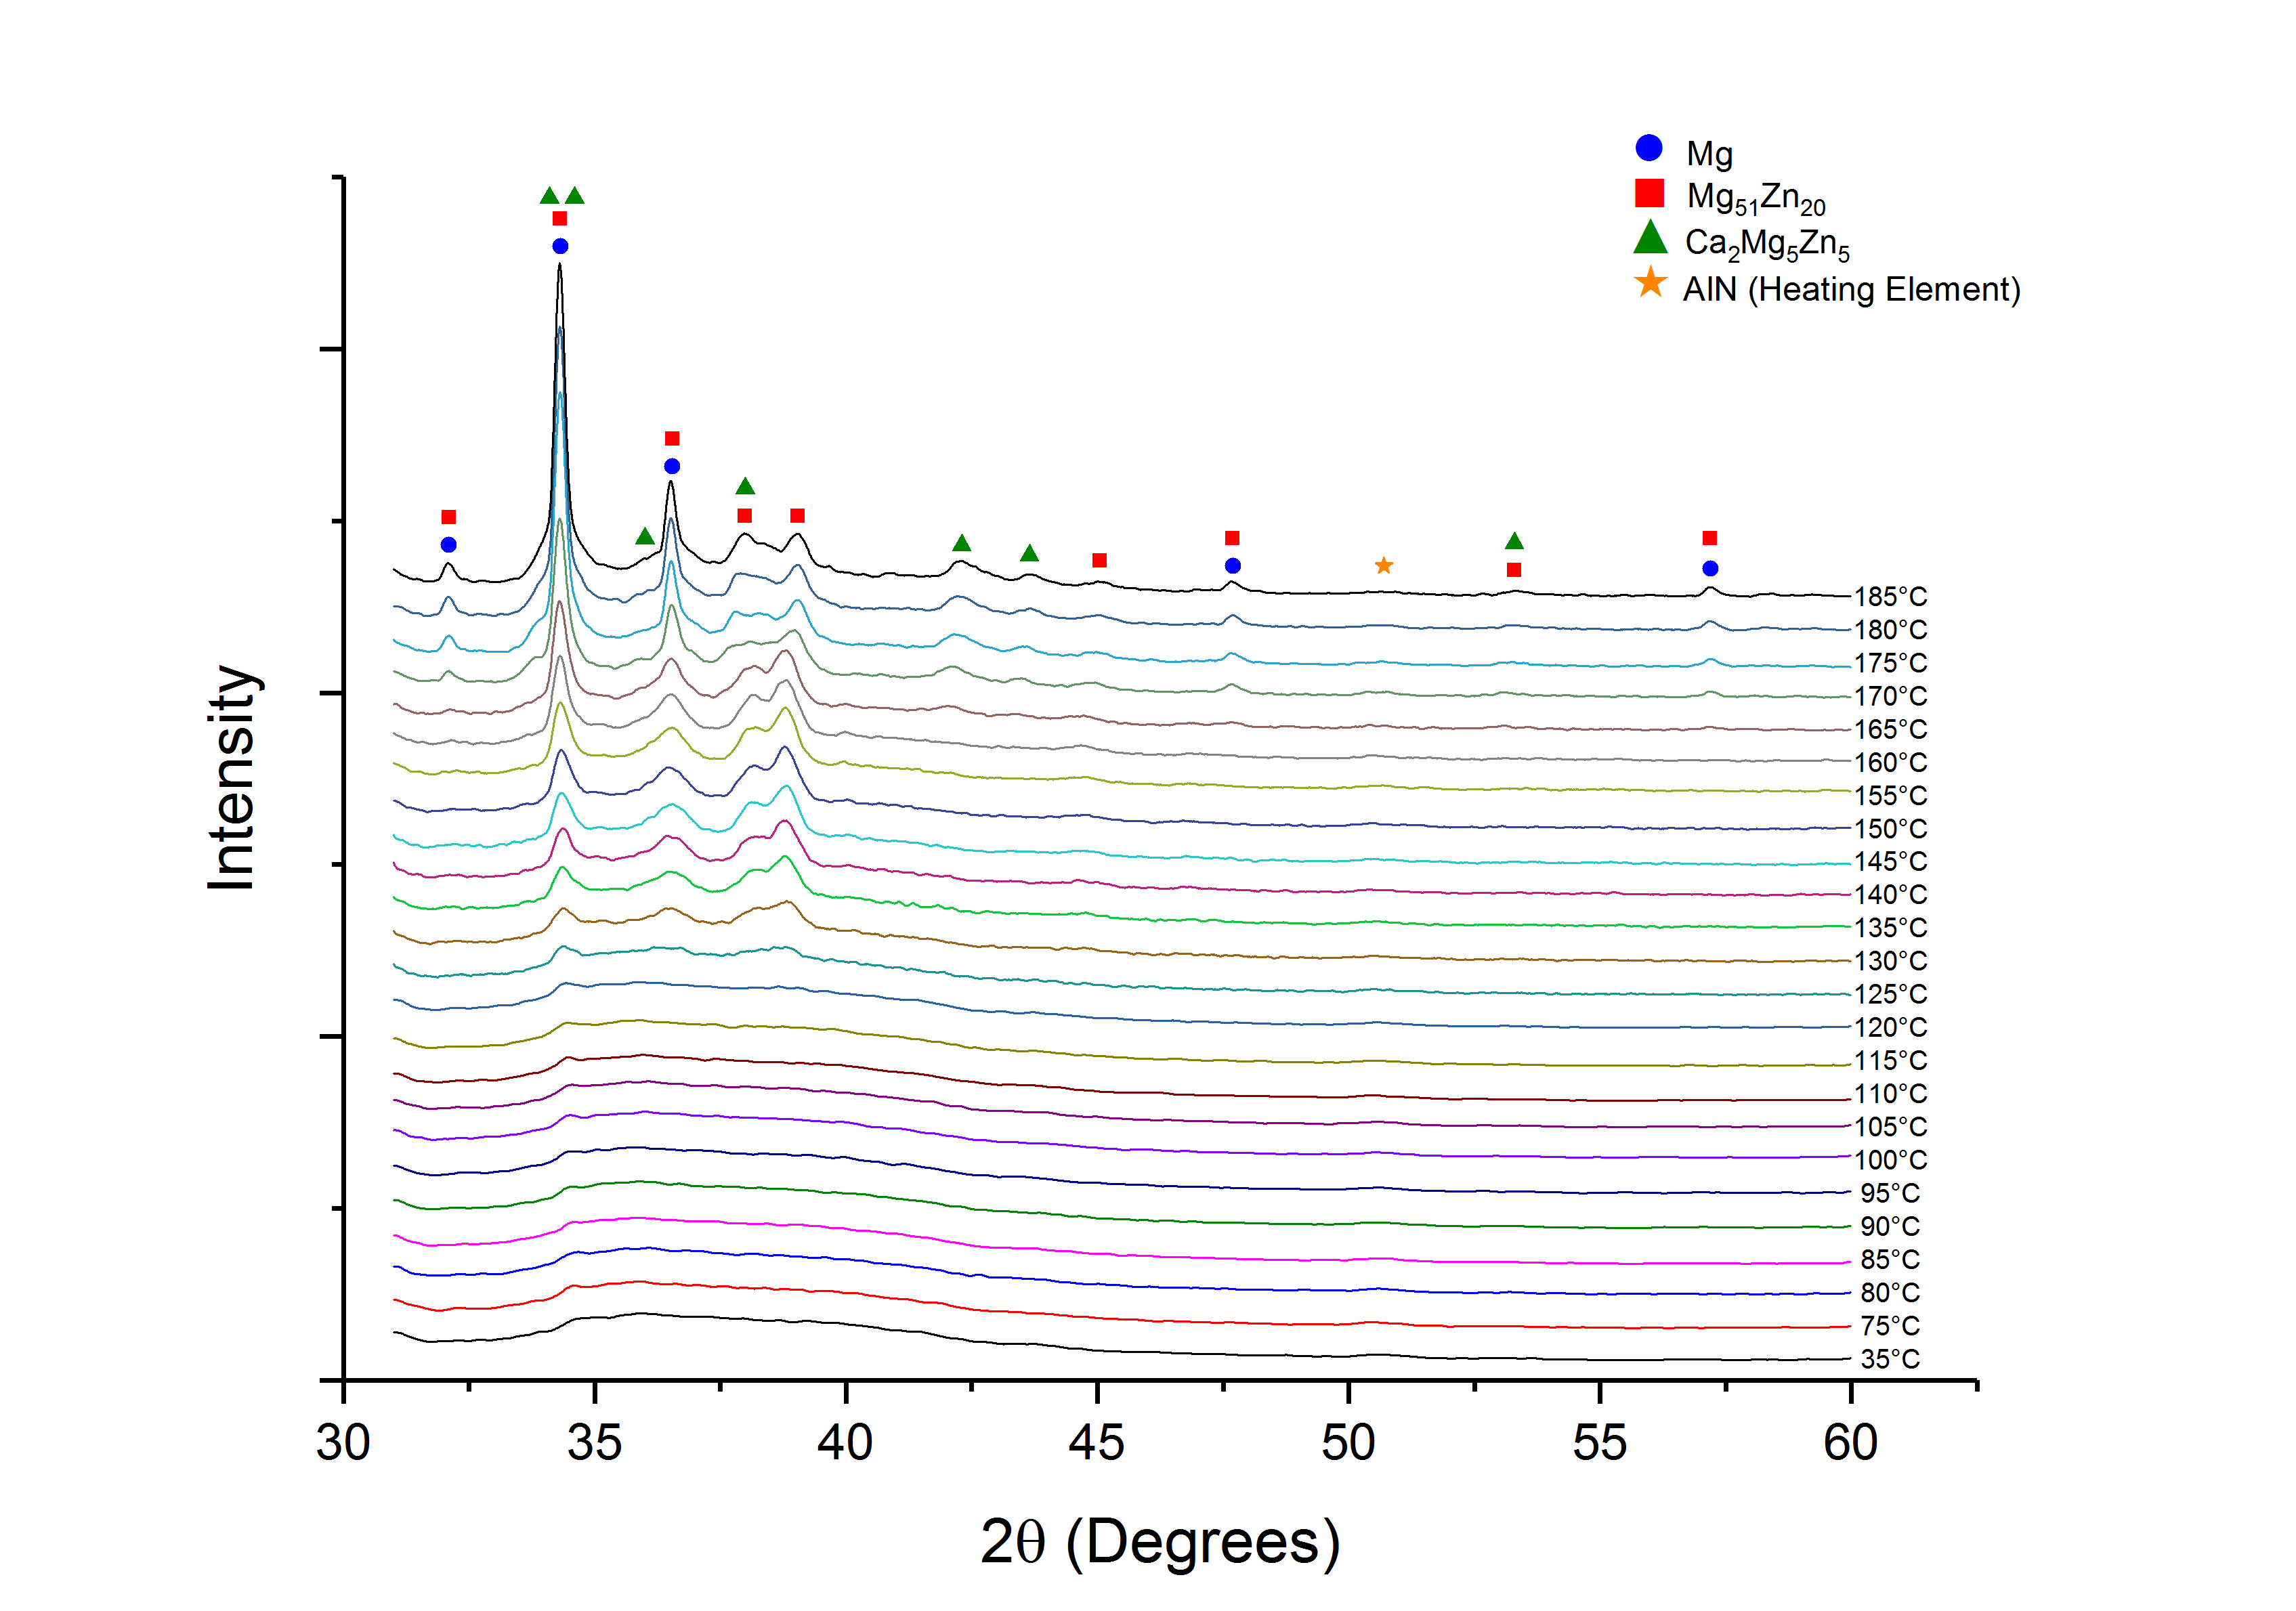
\includegraphics[width=\textwidth]{XRD_Dynamic_Bulk.png}
		\caption{}
		\label{fig:XRD_Dynamic_FullStack_Bulk}
	\end{subfigure}
	%Image 2
	\begin{subfigure}[htbp]{0.75\textwidth}
		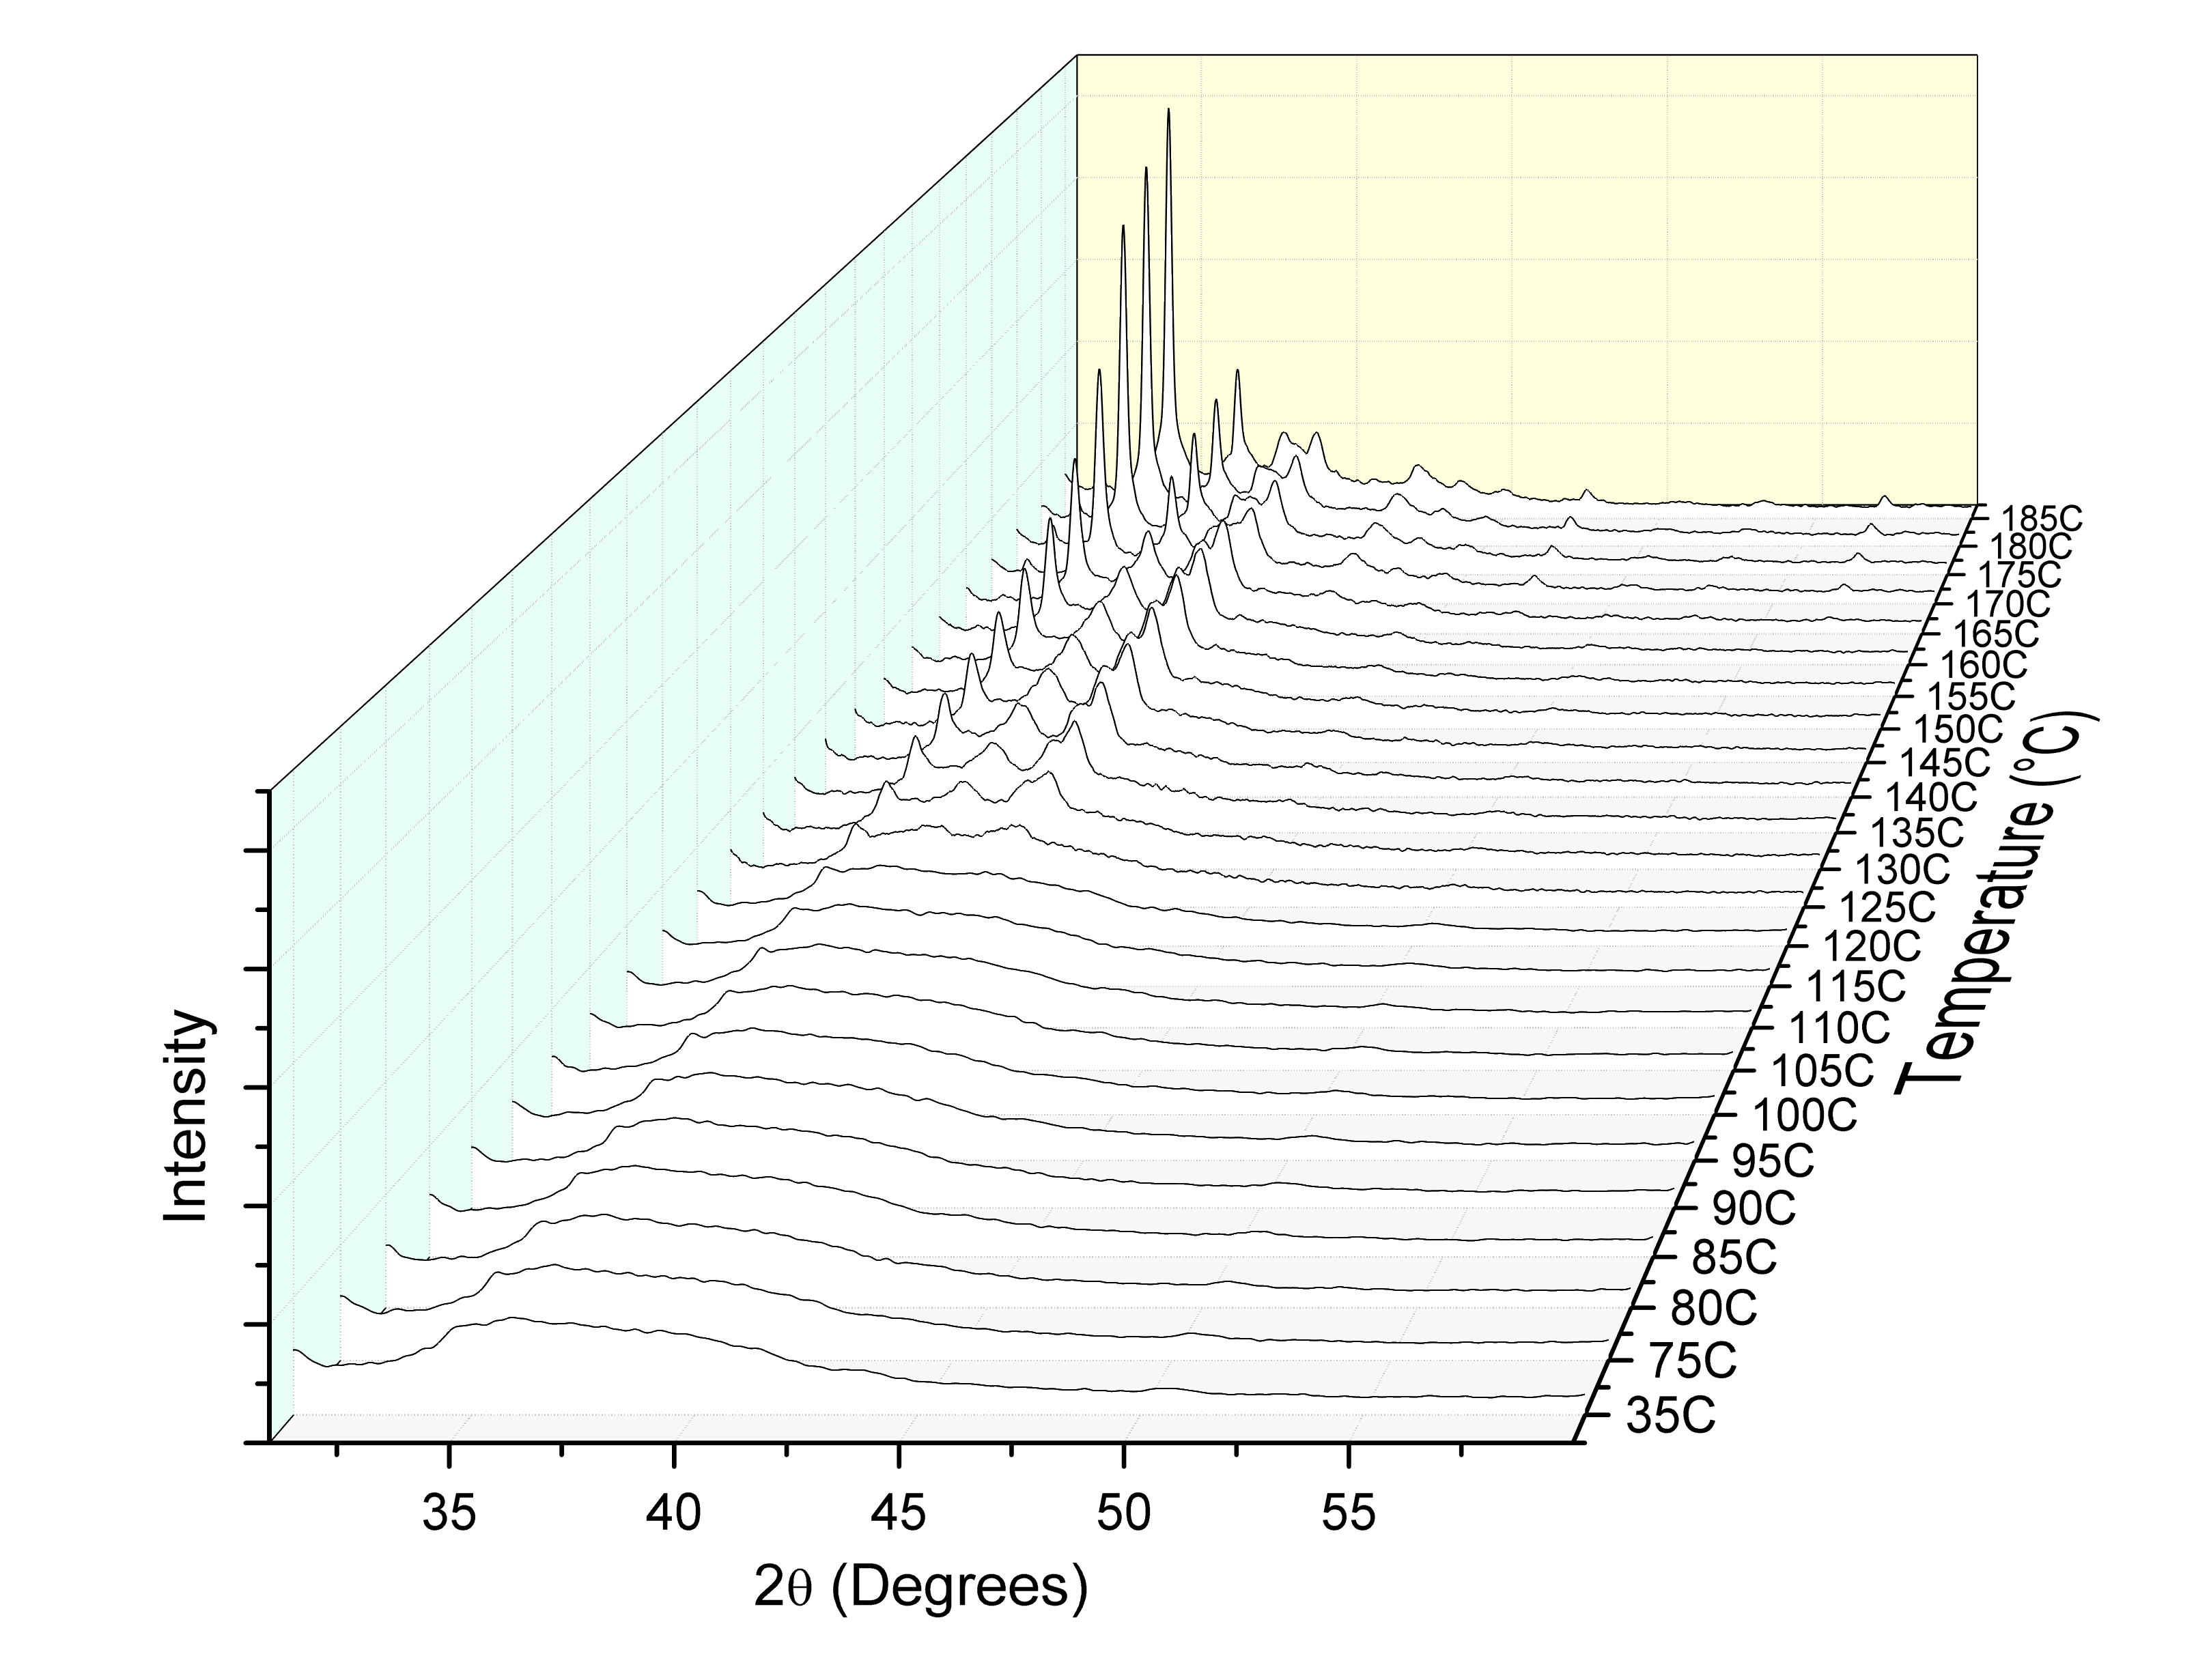
\includegraphics[width=\textwidth]{Bulk_Heated_XRD_Waterfall3D_Smooth2.png}
		\caption{}
		\label{fig:XRD_Dynamic_WaterFall_Bulk}
	\end{subfigure}
	\caption{(a) Stacked \gls{xrd} patterns from the incremental heating of bulk \MgZnCa. (b) Cascading \gls{xrd} patterns from the incremental heating of bulk \MgZnCa. }%global caption
	\label{fig:XRD_Dynamic_Bulk}
\end{figure}

%code to put 2 images side by side in a figure
\begin{figure}[b]
	\centering
	%Image 1
	\begin{subfigure}[htbp]{0.75\textwidth}
		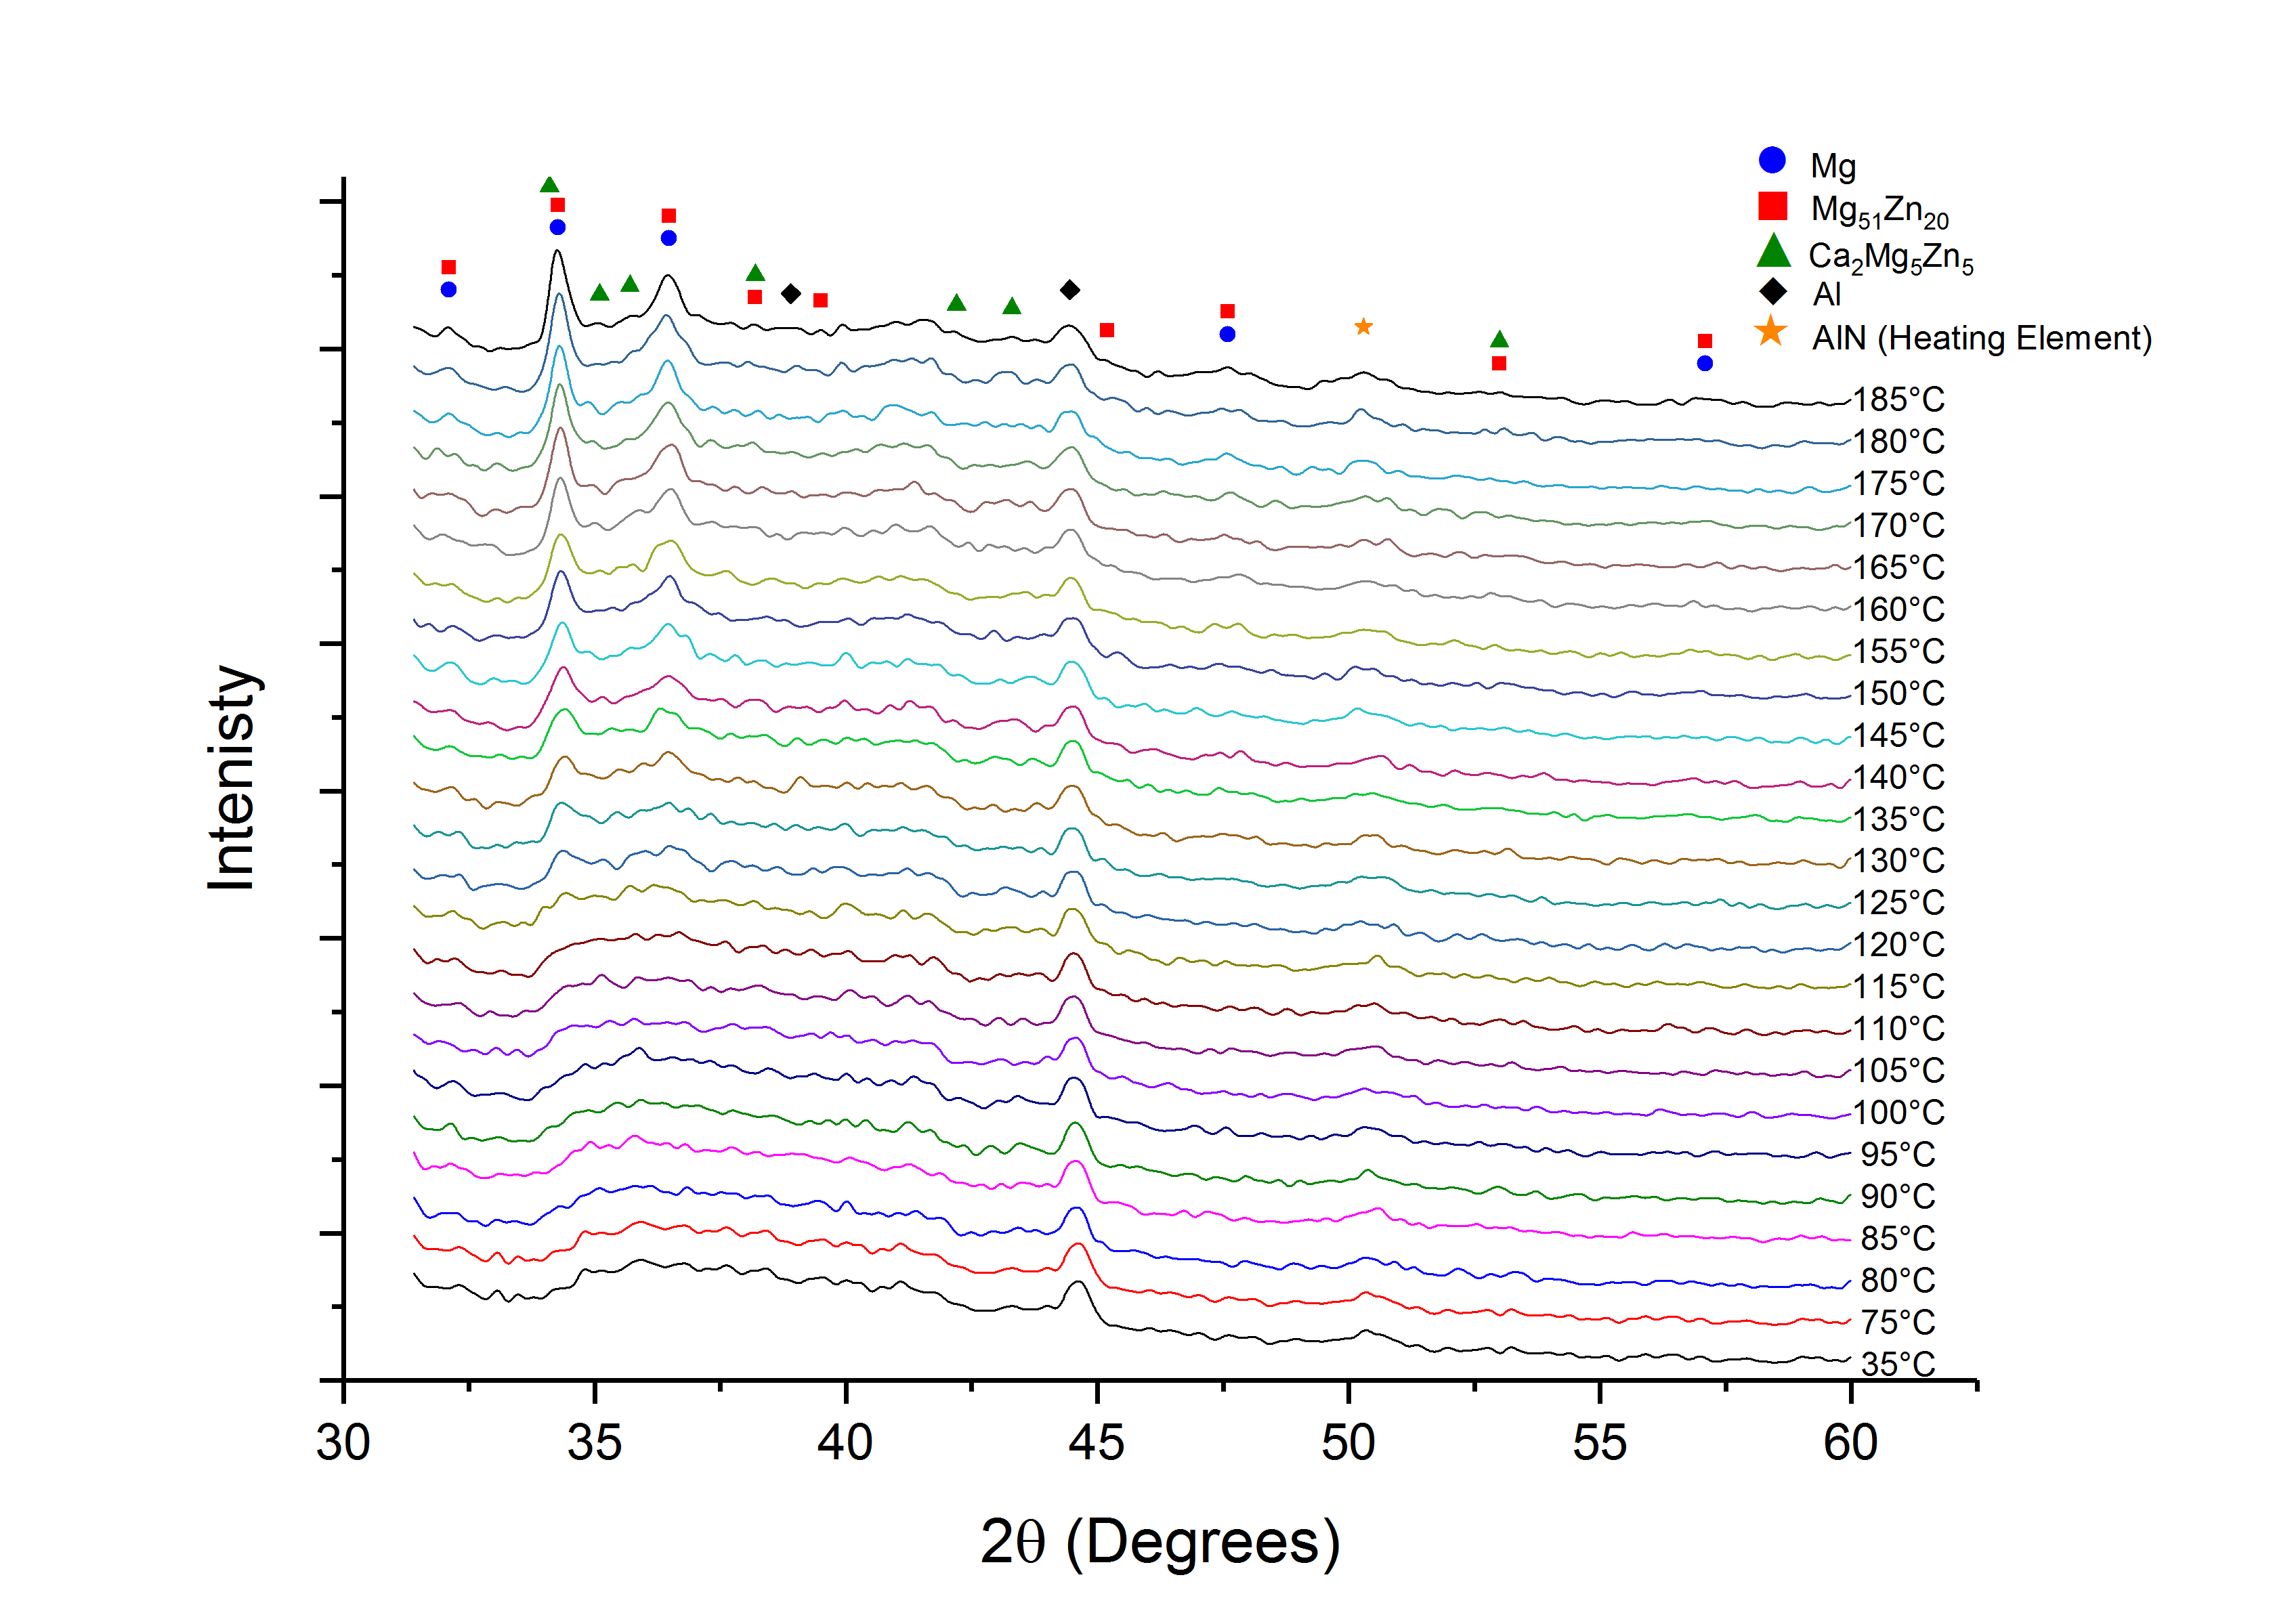
\includegraphics[width=\textwidth]{XRD_Dynamic_Film.png}
		\caption{}
		\label{fig:XRD_Dynamic_FullStack_Film}
	\end{subfigure}
	%Image 2
	\begin{subfigure}[htbp]{0.75\textwidth}
		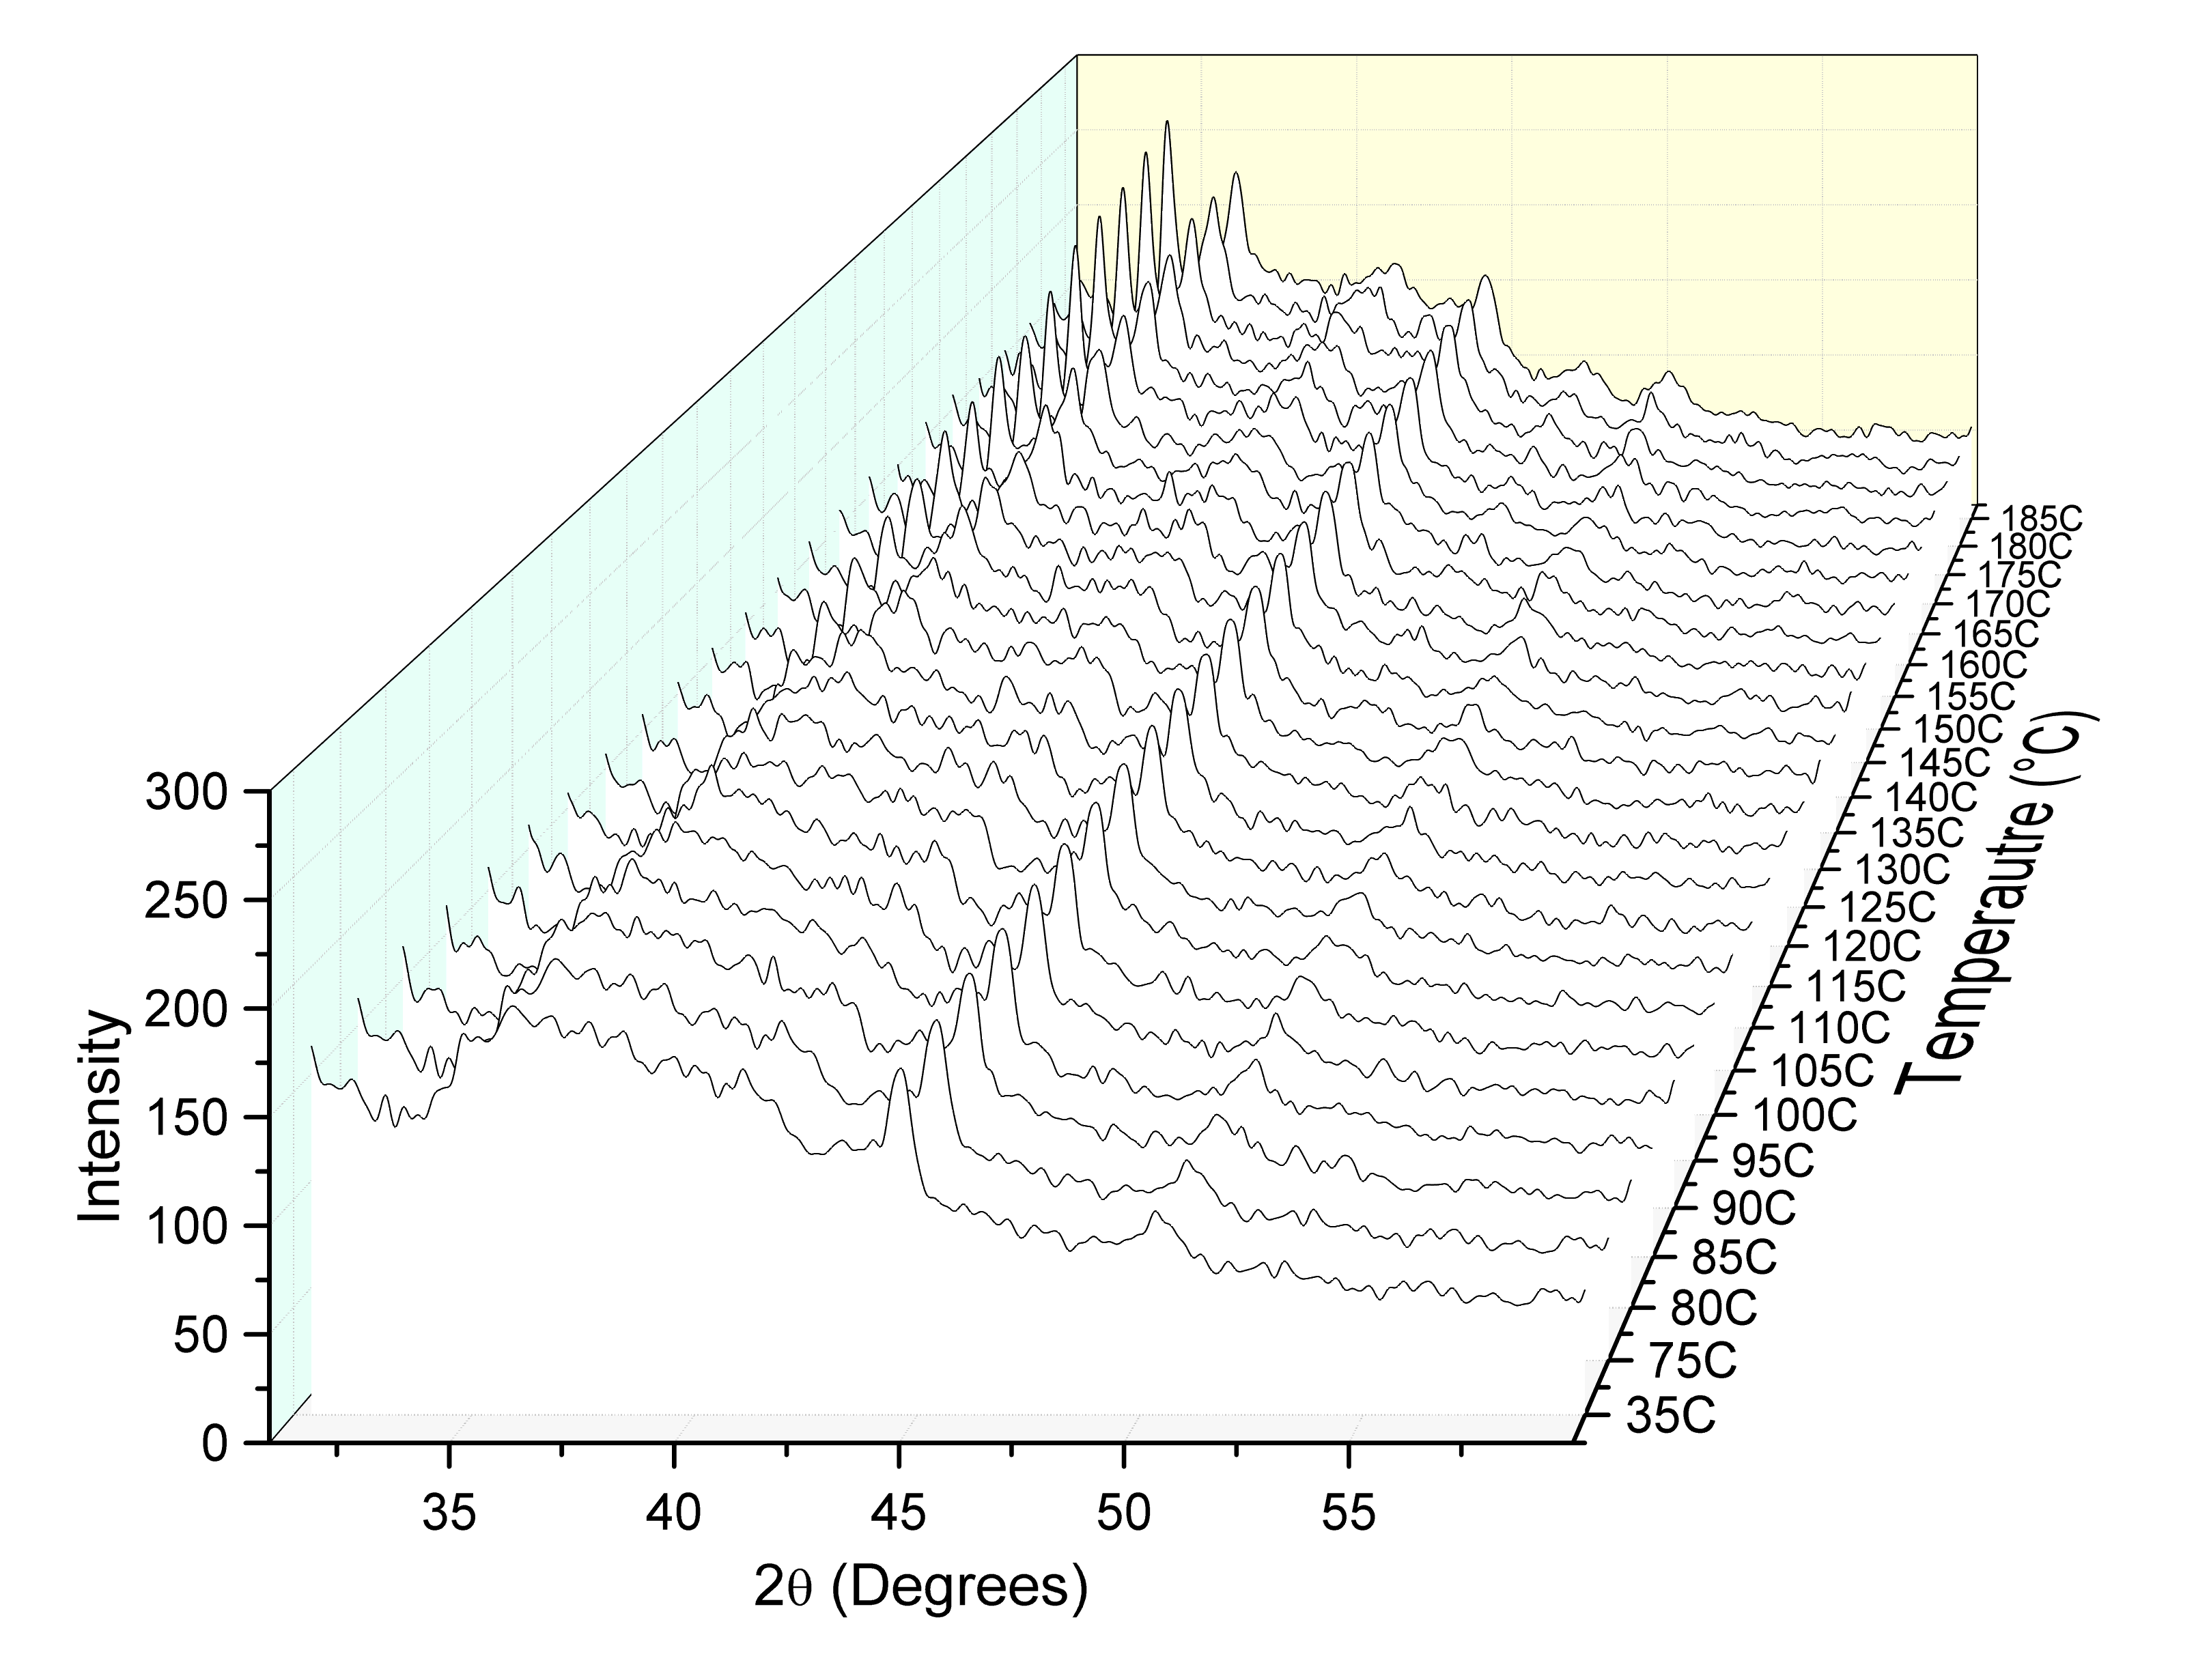
\includegraphics[width=\textwidth]{TF_Facet_HeatXRD_Waterfall3D_Smooth.png}
		\caption{}
		\label{fig:XRD_Dynamic_WaterFall_Film}
	\end{subfigure}
	\caption{(a) Stacked \gls{xrd} patterns from the incremental heating of film \MgZnCa. (b) Cascading \gls{xrd} patterns from the incremental heating of film \MgZnCa. }%global caption
	\label{fig:XRD_Dynamic_Film}
\end{figure}

%%%%%%%%%%%%%%%%%%%%%%%%%%%%%%%%%%%%%%%%%%%%%%%%%%%%%%%%%%%%%%%%%%%%%%%%%%

\section{DISCUSSION}

The use of a 60K \gls{dsc} heating rate compared to the more commonly used 20K rate [sources] shifts peaks for the bulk \MgZnCa~ alloy about 8 - 15 degrees higher. This higher heating rates were used because crystallization events for the films were difficult to differentiation at the lower heating rate. 
Films show little shift to high temperature peaks with increases heating rates, but large shifts with relaxation. 
Bulk show the opposite behaviour, larger peaks shifts with higher heating rates and little shift with relaxation.

%%%%%%%%%%%%%%%%%%%%%%%%%%%%%%%%%%%%%%%%%%%%%%%%%%%%%%%%%%%%%%%%%%%%%%%%%%

\section{CONCLUSIONS}

%%%%%%%%%%%%%%%%%%%%%%%%%%%%%%%%%%%%%%%%%%%%%%%%%%%%%%%%%%%%%%%%%%%%%%%%%%

\section{ACKNOWLEDGEMENTS}

%People
Yu Wang for his assistance with \acrshort{xrd} experimentation and Rietveld refinement. 

%%%%%%%%%%%%%%%%%%%%%%%%%%%%%%%%%%%%%%%%%%%%%%%%%%%%%%%%%%%%%%%%%%%%%%%%%%

%Bibliography
\bibliography{ThesisBib}
\bibliographystyle{unsrt}

%%%%%%%%%%%%%%%%%%%%%%%%%%%%%%%%%%%%%%%%%%%%%%%%%%%%%%%%%%%%%%%%%%%%%%%%%%


\end{document}